%% Use short name MACS, MIS, CIMET, MTDMT, MIXD or MIS
%% Language english or norsk
%% b5paper with oneside or twoside, you can set A4 if you want but you submit in b5

%% If you want print with the heading material on a4 paper you can use this format
%% \documentclass[MACS,english,a4paper,oneside,12pt]{ntnuthesis/ntnuthesis}

%% with the change to using DAIM we have a new option.

\documentclass[MACS,english,DAIM]{ntnuthesis/ntnuthesis}

\usepackage[T1]{fontenc}
\usepackage[utf8]{inputenc}
\usepackage{newunicodechar}
\usepackage[multiple]{footmisc}
\usepackage{textcomp}
\usepackage{graphicx}
\usepackage[hyphens]{url}
\usepackage[hidelinks]{hyperref}

\usepackage{color}
\hypersetup{
    colorlinks=false,
    linkcolor=blue,
    citecolor=blue,
    filecolor=blue,
    urlcolor=blue
}

\usepackage{csvsimple}
\usepackage[numbers]{natbib}
\usepackage{algorithm}
\usepackage{algpseudocode}
\usepackage{amsmath}
\usepackage{array}
\usepackage{tabularx}
\usepackage{makecell}
\usepackage{subcaption}
\usepackage{listings}
\usepackage{chngcntr}
\usepackage[acronym]{glossaries}
\usepackage{siunitx}
\usepackage{pdfpages}

\setlength\extrarowheight{2pt}

\lstset{
    basicstyle=\ttfamily,                   % Code font, Examples: \footnotesize, \ttfamily
    frame=none,                             % A frame around the code
    tabsize=2,                              % Default tab size
    captionpos=b,                           % Caption-position = bottom
    breaklines=true,                        % Automatic line breaking?
    breakatwhitespace=false,                % Automatic breaks only at whitespace?
    showspaces=false,                       % Dont make spaces visible
    showtabs=false,                         % Dont make tabls visible
}
\AtBeginDocument{\counterwithout{lstlisting}{chapter}}
\renewcommand{\lstlistlistingname}{List of Listings}

\makeglossaries

\newacronym{EA}{EA}{evolutionary algorithm}
\newacronym{GE}{GE}{grammatical evolution}
\newacronym{SA}{SA}{simulated annealing}
\newacronym{DGEL}{DGEL}{distribution-based grammatical evolution of L-systems}
\newacronym{DGE}{DGE}{distribution-based grammatical evolution}
\newacronym{GP}{GP}{genetic programming}
\newacronym{GLP}{GLP}{genetic L-system programming}
\newacronym{GA}{GA}{genetic algorithm}
\newacronym{PCG}{PCG}{procedural content generation}
\newacronym{AHP}{AHP}{analytical hierarchy process}
\newacronym{VCS}{VCS}{version control system}
\newacronym{ANN}{ANN}{artificial neural network}

\newglossaryentry{L-system}{name=L-system, description={Lindenmayer systems}}
\newglossaryentry{D0L-system}{name=D0L-system, description={Discrete context free L-systems}}
\newglossaryentry{PD0L-system}{name=PD0L-system, description={Parametric discrete context free L-systems}}
\newglossaryentry{PDIL-system}{name=PDIL-system, description={Parametric discrete context sensitive L-systems}}
\newglossaryentry{branch segment}{name={branch segment}, description={An edge in an interpreted L-system~\cite{2012Prusinkiewicz}}}
\newglossaryentry{internode segment}{name={internode segment}, description={``A branch segment followed by at least one more segment in some path''~\cite{2012Prusinkiewicz}}}
\newglossaryentry{branch base}{name={branch base}, description={A point on a branch with at least two child branch segments~\cite{2012Prusinkiewicz}}}
\newglossaryentry{child segment}{name={child segment}, description={A branch segment following a parent segment in direction from the root}}
\newglossaryentry{parent segment}{name={parent segment}, description={The branch segment a child segment follows}}
\newglossaryentry{straight segment}{name={straight segment}, description={The child segment that continues the branch (as opposed to child segments branching into new branches)~\cite{2012Prusinkiewicz}}}

\begin{document}

% !TEX root = ../Masters.tex
% for students submitting in the DAIM system this information will not be used.
% their is an option for DAIM submission which removes this information and checks it is B5.
% Removing the DAIM option on the document type will use this material.

\setthesistitle{Using L-systems to generate aesthetic plant offspring}
%\setthesisshorttitle{Example Masters Thesis} % a short version for the page headers if your normal title is too long to fit
\setthesisauthor{Magnus Bjerke Vik}
\setthesissupervisor{Mariusz Nowostawski}
%\setthesissupervisorA{Prof. Jon Yngve Hardeberg}  % if you have a second supervisor add it like this


\nmtkeywords{Thesis, Latex, Template, IMT}
%\nmtdesc{This is the short description of a masters thesis}


\setthesisdate{01-06-2017}
\setthesisyear{2017}



%for CIMET theses you need to see all of these as well

%\setthesiscampus{Gj\o{}vik}
%\setthesisHostInstitution{\NTNU}
%\setthesisHostInstitution{University of Eastern Finland}
%\setthesisHostInstitution{Universit\'e Jean Monnet Saint-Etienne}

%\setthesisjuryA{} %jury names
%\setthesisjuryB{} %jury names
%\setthesisjuryC{} %jury names
%\setthesisjuryD{} %jury names


\makefrontpages

%this is the intro to the thesis
%\thesistitlepage % make the ordinary titlepage
\hypersetup{pageanchor=false}
%\include{summary}

\chapter*{Preface}
Here, you give a brief introduction to your work. What it is (e.g., a Master's thesis in AIMT at NTNU, when it was carried out (e.g., during the autumn semester of 2021). If the project has been carried out with a company, you should mention this and also describe the cooperation with the company. You may also describe how the idea to the project was brought up.

You should also specify the assumed background of the readers of this report (who are you writing for).\\[2cm]

%\begin{center}
%\thesiscampus, 
\thesisdate \\[1pc]
\\[1pc]
%\thesisauthor
%\end{center}

% !TEX root = ../Masters.tex
\chapter*{Acknowledgment}
I would like to thank my supervisor, Mariusz Nowostawski, for helping me with his insight, interesting ideas and discussions.
I would also like to thank my girlfriend, Merete Nilssen Ringen, for her support and grammatical fixes.
Finally I would like to thank my classmates for making the process of writing the thesis a bit more fun.

% I would like to thank the following persons for their great help during \ldots
%
% If the project has been carried out in cooperation with an external partner (e.g., a company), you should acknowledge the contribution and give thanks to the involved persons.
%
% You should also acknowledge the contributions made by your supervisor(s).

\begin{flushright}
M.B.V.\\[1pc]
\end{flushright}


% !TEX root = ../Masters.tex
\chapter*{Abstract}

This thesis explores how to improve L-system plant generation using \glspl{EA}.
The plants should be aesthetically pleasing, varied, and have the ability to be combined with other plants.

Previous work has shown that simple \glspl{D0L-system}, \glspl{PD0L-system} and \glspl{PDIL-system} can be evolved using \glspl{EA} both autonomously and interactively.
The \gls{L-system} grammar used is simple, restricting the possible solutions.
Additionally often only parts of the grammar is represented in the genotype that is used in the \gls{EA}, thus limiting the evolution.

More complex \glspl{L-system} are required to generate aesthetically pleasing and varied plants, but this also complicates the generator and therefore also the evolution.
To mitigate this issue, \gls{DGEL} is introduced and implemented.
It is based on \gls{GE} of \glspl{L-system}, but introduces a grammar distribution to control what parts of the grammar that should have a higher priority.
\Gls{SA} is used to optimize this grammar distribution so that \gls{DGEL} can produce well performing plants in a more efficient manner.
Additionally, using different optimized grammar distributions could allow for a larger variety of plants, while still keeping the quality up.
Fitness metrics used were both adapted from the reviewed literature and created from scratch to assess the pleasingness of the generated L-system plants.

\Gls{DGEL} was evaluated in three parts: \gls{GE}, \gls{SA} and fitness function.
Plain \gls{GE} was tested against a random brute-force approach to see if it has any benefit.
\Gls{SA}s progress and produced grammar distribution was studied in depth, and its performance was compared in multiple ways using both \gls{GE} and random brute-force approaches.
The fitness metric was compared to human evaluations of generated L-system plants through \gls{AHP} and rank correlation statistics.
Additionally, it was analyzed what factors humans think are important for distinguishing good from bad plants.
\Gls{GE} was found to be superior to brute-force.
\Gls{SA} was found to improve the efficiency of both brute-force and \gls{GE}.
Finally, the fitness function was found to not match the human evaluation, but a small correlation was still present.

The findings suggest that \gls{DGEL} can improve the efficiency of generating L-system plants in a complex space. In a more general sense, the findings suggest that accompanying an EA with a probability distribution, and optimizing it using optimization techniques, can improve its efficiency in complex spaces, allowing for faster searches and more varied solutions.

\hypersetup{pageanchor=false}




\tableofcontents

\hypersetup{pageanchor=true}

\listoffigures
\listoftables
\lstlistoflistings
\printglossaries

\chapter{Introduction}
\label{chap:introduction}

\section{Topic covered by the project}
In the area of computer graphics and visualization, there is a desire to replicate environments and creatures found in nature in a virtual environment.
All types of environments and creatures are of interests.
Some examples are terrain, mountains, rivers, plants, animals and bacteria.
These can be recreated by manually modeling the specific objects, but to be able to represent the large variations of the objects, this method is tedious and costly.
Another approach to solve this is to procedurally generate the content using procedural content generation (PCG) methods.
This way, digital programs can generate virtually infinite amounts of variations based on a representation and a recipe.

Plants can be generated using L-Systems~\cite{2012Prusinkiewicz}, where their structure is represented as strings of characters in a parallel rewrite system.
Based on actual plants, one may model a virtual plant by creating the rewrite rules and parameters for how the system should be drawn.
Alternatively, it is possible to generate new plant species by using genetic algorithms and natural selection.

\section{Keywords}
L-system, plant, procedural content generation, PCG, genetic algorithm, feature extraction.

\section{Problem description}
\label{sec:ProblemDescription}
% Should add some sources.
Plants can be cross-bred and selected to create offspring with desirable features from multiple species.
For example, most of the species used in agriculture have gone through selection and cross-breeding over several years to yield species that produce a bigger quantity of food and are resistant to deceases and harsh environments.
This can be a long process, taking several hundred of years with gradual improvements, and many combinations do not even work.
To make this process more fun and interesting, a virtual world where people can cross-breed plants can be created.
In this world, cross-breeding is not limited like it is in the real world.
Plants could be combined in ways never possible in the real world.
For example, a user may like both apple trees and Venus flytraps, so they want to combine them into a tree with Venus flytrap mouths that could eat humans.
The problem here is that randomly crossing the representation of different plants may not produce meaningful or interesting offsprings, but rather random creatures that do not satisfy the user.

\section{Justification, motivation and benefit}
Solving this problem will create the foundation for multiple games based on or using cross-breeding of plants.
Additionally, it may be possible to generalize the results to other areas of cross-breeding and PCG, such as breeding animals, or generating levels.
Creating a game based on cross-breeding where the offsprings may be disliked by the users may be catastrophic and result in a game that will not make any revenue.

The results from this research can be used in a game where users may create their own virtual garden, potentially in virtual reality (VR), where they breed the plants they always wanted to see or new surprising species, and have a place outside the busy world to relax and watch their plants grow.
The research results will directly benefit game developers wishing to create games like the one described, and indirectly benefit the PCG research community, other game areas, users of the produced games and companies developing and publishing games.
The game developers and publishers will benefit from more revenue by producing new and interesting games, while users will benefit from new games that fulfill their entertainment and relaxation needs.

\section{Research questions}
The problem described can be summarized in a single research question: How can plant L-systems be combined into offspring that humans find at least as aesthetically pleasing as its parents?
As L-systems can be used to generate various types of shapes, not only plants, ``plant L-systems'' is used as a term meaning L-systems used for generating plants.
To avoid having to reuse the term ``plant L-system'', the term ``L-system'' from this point on mean specifically L-systems to generate plants in the context of the problem.
A hypothesis to this question is that if distinct features from both parents are included in the offspring, the offspring should be at least as pleasing as its parents.
Thus, the initial question can be split into two more specific sub questions: How can L-systems be combined to create offspring with distinct features from both parents, and how aesthetically pleasing are the generated offspring compared to their parents?

To discover how L-systems can be combined with features from both parents, some more knowledge is needed.
First, the L-systems should be able to represent plants both found in nature and not found in nature, as the problem involves combining existing plants into new plants.
Thus a new research question is defined: What types of L-systems are appropriate to represent plants both found in nature and not found in nature?
To combine the L-systems together into offspring with distinct features from both parents, features in an L-systems that appropriately reflect the features found in the produced plants need to be identified.
This gives raise to the question: What are the features of an L-system that can be combined?
Finally, the combination of the features needs to happen, and thus comes the question: How can the features be combined to create offspring that contain distinct features from both parents?

In the end, there is one main research question, and four sub questions that aim to answer the main question.
The questions are listed below.
It is important to notice that these questions can not be answered individually, but as a sequence where the next question depends on the previous.

\begin{description}
    \item[RQ0] How can plant L-systems be combined into offspring that humans find at least as aesthetically pleasing as its parents?
    \begin{description}
        \item[RQ1] What types of L-systems are appropriate to represent plants both found in nature and not found in nature?
        \item[RQ2] What are the features of an L-system that can be combined?
        \item[RQ3] How can the features be combined to create offspring that contain distinct features from both parents?
        \item[RQ4] How aesthetically pleasing are the resulting plants compared to their parents?
    \end{description}
\end{description}

\section{Contribution}
\begin{itemize}
    \item A literature review of L-system representations and features of those representations.
    \item A proposed algorithm for how to combine L-systems while retaining distinct features from both parents.
    \item A software implementation of the algorithm that can take two L-systems and combine them into a new L-system.
    \item An analysis of how well users perceive the combination of plants using the algorithm.
\end{itemize}

% !TEX root = ../Masters.tex
\chapter{L-system Representation and Evolution}

\section{L-systems}
\glspl{L-system} was introduced by Lindenmayer in 1968 as a ``theoretical framework for studying the development of simple multicellular organisms''~\cite{2012Prusinkiewicz}, and then later applied to model plants.
An \gls{L-system} consists of an alphabet, an axiom and a set of production rules.
It is a parallel rewrite system where each letter in the axiom word is rewritten independently based on the production rules.
This happens iteratively, where a new word replaces the previous word each iteration.
A way to draw the plant based on the \gls{L-system} has to be applied to visualize it.
Prusinkiewicz and Lindenmayer summarize multiple research papers into a comprehensive book about \glspl{L-system}~\cite{2012Prusinkiewicz}.
For a more comprehensive and in-depth explanation of \glspl{L-system}, refer to this book.

There are also multiple types of \glspl{L-system}, including discrete, stochastic, context sensitive and parametric~\cite{2012Prusinkiewicz}.
All of these can be combined into one \gls{L-system}.
A stochastic, context sensitive and parametric \gls{L-system} (parametric S2L-System) can model all of the other types of \gls{L-system} by having 100\% probabilities (discrete), no contexts or no parameters, and is thus the most flexible representation.

Discrete context-free \glspl{L-system} (D0L-systems) are the simplest \glspl{L-system}, and can be created using edge rewriting, node rewriting, or both~\cite{2012Prusinkiewicz}.
In these systems, there exists one production rule per letter in the alphabet.
By default the productions will produce the same letter as the input (identity).

Stochastic \glspl{L-system} add a randomness to the generation of the plants.
Each letter in the alphabet may have multiple productions, each with a probability of being selected~\cite{2012Prusinkiewicz}.
This may simulate how different instances of a plant species may look slightly different, thus making the plants look less synthetic when seen together with other plants of the same species.

% Xueqiang and Hong developed a generalized L-system method, called GLSM, that better follows botanical principles and increases the expressive ability of L-systems.
% They emphasize the importance of a stochastic property in the L-systems to reflect botanical principles.~\cite{2012Xueqiang}

% Wensheng and Xinyan model grass with stochastic L-systems and trees with parametric L-systems~\cite{2010Wensheng}.
% For the tree models, they create one L-system where four parameters determine the branching angles and branch lengths.
% They show how two different set of parameters in the same L-system can generate two different looking trees, and how adding stochastic multiples to the parameters can generate more naturally looking trees.
% This is different from stochastic L-systems, because here they multiply stochastic values with parameters in the productions, while stochastic L-systems select productions stochastically.

Context sensitive \glspl{L-system} add a context to the production rule.
The context can be on either left, right or both sides of the letter.
A production will only be used if the context matches the surrounding letters in the word.
With this, signal propagation can be simulated either upwards or downwards through the plant~\cite{2012Prusinkiewicz}, and more complex plants may be generated.

Parametric \glspl{L-system} adds parameters to the letters in the words, and conditional rules~\cite{2012Prusinkiewicz}.
The main benefit of using parametric \glspl{L-system}, is that it can work with rational numbers rather than only integers.
For example, with non-parametric \glspl{L-system}, extension of a segment can be modeled with the rule $F\rightarrow FF$, or any number of ``F'' in the successor.
In any case, it will only be possible to grow the segment with a multiple of the previous.
For some plants, this is enough, but to model a larger variety of plants, rational numbers are required.
With parametric \glspl{L-system}, the same rule would be $F(l)\rightarrow F(l*2)$, where $l$ is the length of the segment.
But now it is also possible to grow it at another rate, e.g.\ $F(l)\rightarrow F(l*1.2)$.
Prusinkiewicz and Lindenmayer describe more of the benefits of parametric \glspl{L-system}~\cite{2012Prusinkiewicz}.

Prusinkiewicz describe \glspl{L-system} as having three levels of model specification: partial \glspl{L-system}, \gls{L-system} schemata, and complete \glspl{L-system}~\cite{2012Prusinkiewicz}.
The three different levels go from more abstract to more concrete, where partial \glspl{L-system} specify which structures may result into which new structures (e.g.\ bud becomes a flower), schemata specifies when the different structure switches happen (e.g.\ when the bud becomes a flower), and complete systems specify the geometry of the plant to be visualized (e.g.\ how the bud and the flower should look).
Different methods exist for each level, and which method to use will depend on the type of plant that should be generated.

\gls{L-system} schemata is of particular interest because there exists multiple methods to use.
The event of a structure resulting into a new structure is called a {\it developmental switch}~\cite{2012Prusinkiewicz}.
The timing of the switches need to be controlled by a control mechanism in the system.
There are two classes of these mechanisms: lineage and interaction.
Lineage mechanisms are transferring information from a module to a descendant, while interaction mechanisms exchange information between cells.

Prusinkiewicz and Lindenmayer describe some of the mechanisms used.
The stochastic mechanism uses a stochastic \gls{L-system} to apply probabilities to developmental switches.
A table \gls{L-system} has multiple tables with different rules that can be applied depending on some external factor.
For example, one table can represent summer and another can represent winter, making different switches happen at different seasons.
The delay mechanism can delay the developmental switch by a specified number of iterations, for example making a flower bud bloom after a certain amount of iterations.
Accumulation of components uses parametric \glspl{L-system} to accumulate some parameter until it reaches a threshold causing the switch to happen.
Parametric \glspl{L-system} can also be used to control development switches with signals, where a signal travels either upwards or downwards through the plant.~\cite{2012Prusinkiewicz}

A popular way to render complete \glspl{L-system} is the turtle interpretation, where a cursor (the turtle) follows instructions to draw lines, and the alphabet is the set of instructions to use~\cite{2012Prusinkiewicz}.
Turtle interpretation is in its original form simple and can only draw lines on a 2D image, but it has been extended to draw realistic looking plants in 3D~\cite{2012Prusinkiewicz}.
To use the turtle interpretation, extra parameters describing how much the \gls{L-system} should be expanded and how it should be drawn has to be defined~\cite{2012Prusinkiewicz}.
For example, the number of rewrite iterations, the branching angle, the segment length, and the segment width have to be specified.
This may depend on the plant to be rendered, as some plants might require a more complex set of drawing instructions.

\section{Genetically Evolving L-systems}
Genetic evolution involves crossing and mutating genes from parents to create offspring.
Thus, the research field of \gls{L-system} genetic evolution is a good starting point for finding out both how to generate \glspl{L-system} and combine them.
A set of research papers published between 1995 and 2013 was studied to see what different techniques have been used.

When evolving objects, an \gls{EA} is often used.
\gls{EA} is composed of a series of steps that will evolve a population over multiple generations based on some criteria.
It begins by generating an initial population of individuals.
Then it evaluates the individuals with a fitness function.
This is then used to select the best individuals to be used for reproduction.
The individuals are then used to create offspring for a new population by using crossover and mutation.
Finally, the new population is evaluated and the steps repeat.
In the context of \glspl{L-system}, the \textit{object} will be replaced with \gls{L-system}.

To get a better overview of the \gls{EA} techniques used for \glspl{L-system}, the \gls{EA} has been split into five parts: model, representation, generation, selection, and genetic operators.
The \textit{model} and \textit{representation} are related and sometimes almost equal.
The difference is that the model describes how the plant is modeled, while the representation may be a small part of the model or the model represented in a different format, and is the part which is evolved by the algorithm.
\textit{Generation} is how the representations are generated, e.g.\ for the initial population, or when replacing parts of an \gls{L-system} with a new part.
\textit{Selection} is the part of selecting individuals to be used for creating the next generation.
\textit{Genetic operators} are used on the selected individuals to modify the representation by either doing crossover between parents, mutating an offspring, or other.

\subsection{Model}
Discrete context-free \glspl{L-system} (D0L-systems) are the simplest form of \glspl{L-system} and they are commonly used for \gls{EA}~\cite{1998Mock,1998Ochoa,2002Ebner,2003Ebner,2006Ashlock,2009Beaumont,2009Corchado}.
Parametric discrete context-free \glspl{L-system} (PD0L-systems) have also been prominently used in the literature~\cite{1994Jacob,2000Vanak,2001Hornby}.
Parametric discrete context-sensitive \glspl{L-system} (PDIL-systems) have been used in Jacob's further work by extending the PD0L-system version~\cite{1995Jacob, 1996Jacob, 1996Jacob-2}.
Other types of \glspl{L-system}, such as stochastic, timed, table, environmentally-sensitive and open \glspl{L-system} have not been used for \gls{EA} in the reviewed literature.
Hornby and Pollack argue that stochastic \glspl{L-system} are hard to use for \gls{EA} because they are non-deterministic~\cite{2001Hornby}.
Additionally, they argue that context-sensitive \glspl{L-system} are not as powerful as parametric \glspl{L-system}, and should thus not be used.
They use PD0L-systems in their own research, but it is worth noting that they evolve moving creatures rather than plants.

All of the above-mentioned \glspl{L-system} are bracketed \glspl{L-system}, i.e.\ they include stack operators (\texttt{[} and \texttt{]}) in their alphabets to push and pop the current interpretation state, which creates branches in the structure.
Additionally, Hornby and Pollack use repetition brackets (\texttt{\{} and \texttt{\}}) with an integer parameter to specify how many times the content inside the brackets should be repeated~\cite{2001Hornby}.

The \gls{L-system} type is only the first part of the model required to model a plant.
The second and final part is the interpretation of the \gls{L-system} into a visualized model.
Even though the literature only use three types of \glspl{L-system} (D0L, PD0L and PDIL), they use different ways of interpreting it.
Both Mock, Ochoa, and Beaumont and Stepney visualize the \glspl{L-system} in 2D with branching, but while Mock uses node rewriting~\cite{1998Mock}, Ochoa and Beaumont and Stepney use edge rewriting~\cite{1998Ochoa,2009Beaumont}, which results in different types of plants.
The remaining authors use 3D visualization with branching~\cite{1994Jacob,2006Ashlock}, though Jacob adds the concepts of sprout, stalk leaf and bloom~\cite{1995Jacob}, and Ebner et al.\ only add leaves~\cite{2002Ebner,2003Ebner}.

\subsection{Representation}
The representation used for \gls{EA} also varies.
In the literature, there have been three main \gls{EA} methods: \gls{GP}, \gls{GA} and \gls{GE}.
Jacob and Ochoa use the \gls{GP} methods~\cite{1994Jacob,1995Jacob,1998Ochoa}, both based on techniques introduced by Koza~\cite{1992Koza}.
Ochoa uses a simple version of \gls{GP}, where representation only consists of one single rule successor~\cite{1998Ochoa}.
The successor is divided into a hierarchy based on the branching in the string, such that top-level letters are on the top, and each stack below is one level down.
In their paper, they only use successors with one level deep branching.

Jacob represents the whole \gls{L-system} as a tree structure, such as a \gls{GP} method commonly does~\cite{1994Jacob}.
The tree structure starts with the \gls{L-system} root at the top, then with the axiom and rules as children, then with each rule as a child of rules.
The axiom has one child for each letter, and each letter has a child for the parameter.
Each rule have a left and right side, where the left is the predecessor and the right is the successor.
The left node is composed the same way as the axiom, but without parameters.
The right node is also the same, but it can have parameters and also stacks for branching that also follow a tree structure.
It can practically represent any PD0L-system this way, but without conditions and with a limited set of letters.
This could be extended.

\gls{GA} is the second major method used in the literature.
The main difference between \gls{GA} and \gls{GP} is that \gls{GA} represents the genotype as a flat string of elements, while \gls{GP} represents it as a tree structure.
Both Mock, Ochoa and Corchado et al.\ use only a single rule successor to represent the genotype~\cite{1998Mock,1998Ochoa,2009Corchado}.
The successor is a plain string of symbols, including letters and the branching operators.
While Ochoa only uses node rewriting~\cite{1998Ochoa}, Mock and Corchado et al.\ only use edge rewriting~\cite{1998Mock, 2009Corchado}.

Ebner et al.\ represent the genotype as a set of production rules with one edge rewriting rule and 0--26 node rewriting rules, each with individual nodes ranging from A--Z~\cite{2002Ebner,2003Ebner}.
The predecessor is fixed based on the rule number.
For example, the first rule predecessor is always \texttt{f}, while the second and third predecessors would be \texttt{A} and \texttt{B}.
This means that the genotype is a set of strings (successors), instead of one single string.
This would allow the \gls{GA} to search a bigger space compared to Mock and Ochoa's genotypes.

Hornby and Pollack take this further and represent the genotype as a fixed number of production rules composed of a predecessor and successor~\cite{2001Hornby}.
In this case, the genotype has as set of pairs of strings, which would allow the \gls{GA} to search a even bigger space.

Finally, Ashlock et al.\ encodes the \gls{L-system} as a string of real numbers~\cite{2006Ashlock}.
Some of numbers encoded are used to index a table of a fixed set of \gls{L-system} rules, and some are used directly in the \gls{L-system} interpretation step.
This enables the \gls{L-system} and its interpretation to be tackled as one single parameter optimization problem.
None of the previous genotypes presented represented the \gls{L-system} interpretation, though Ebner et al. and Hornby and Pollock used PD0L-systems where some interpretation parameters can be moved into the \gls{L-system} production strings.
Even though the encoded genotype can affect more aspects of the \gls{L-system} (rules and interpretation), it is more limited because of its fixed set of rules that are used.
Thus it can search a smaller space than Hornby and Pollack's representation.

\gls{GE} is the final and latest method used in the literature.
It is ``an [\gls{EA}] that can evolve complete programs in an arbitrary language using a variable-length binary string''~\cite{2003Oneil}.
It was introduced for \glspl{L-system} by Ortega et al. to evolve a D0L-system into fractal curves~\cite{2003Ortega}.
Beaumont and Stepney transferred this to generating D0L-system 2D plants to match a drawing of a plant~\cite{2009Beaumont}.
Interestingly, \glspl{L-system} themselves are grammar that produce plants, but Beaumont and Stepney's work defines a grammar that produce the \glspl{L-system}, which then is used to produce the plant.
They represent the genome as a string of numbers that index into a Backus Naur Form (BNF) grammar to build the \gls{L-system}.
In this sense the representation is similar to that of Ashlock~\cite{2006Ashlock}, but with integers instead of real numbers and a different way of mapping from numbers to the \gls{L-system}.
It is also similar to Jacob's \gls{GP} representation because it uses a pool of expressions that could be compared to a BNF.
When undergoing evolution, the genotype (string of numbers) will be modified by a \gls{GA}.
Thus the \gls{GE} method is strongly related to \gls{GA}.

Beaumont and Stepney use a limited search space for the \gls{GE} method.
Their alphabet only consists of \texttt{F}, \texttt{+} and \texttt{-}, their axiom is always \texttt{F}, and only \texttt{F} can be the production predecessor, i.e.\ it is an edge rewriting \gls{L-system}.
They also have a fixed number of iterations and rotation angle.
This can be expanded, and they did some experiments to try this.
\texttt{+} and \texttt{-} was added as predecessor letters, and the axiom was allowed to contain any symbols and have any length.
This expanded the search space, making the algorithm find fewer very bad solutions, but also far fewer good solutions.
Finally, they added a second terminal symbol \texttt{X} in addition to \texttt{F}, allowing for both edge and node rewriting \glspl{L-system}.
This further expanded the search space, but required a significantly larger population size and more generations, making the computation time significantly longer.
The search space for this \gls{GE} representation is smaller than some of the other methods because of its use of non-parametric \glspl{L-system} and limited set of symbols, but it could be expanded to include this.

In addition, there is a non-\gls{EA} method introduced by Vanak that still is relevant, called XL-system~\cite{2000Vanak}.
Rather than evolving \glspl{L-system}, the XL-system is another form of \glspl{L-system} where two or more PD0L-systems are combined with an X-machine into an XL-system.
The original \glspl{L-system} are not modified in any way, but rather kept as two states in the X-machine.
The XL-system is used as a normal \gls{L-system}, running a specified amount of derivations to rewrite an axiom.
The difference is that the XL-system switches between the contained \glspl{L-system} based on specified conditions while iterating.
The active \gls{L-system} is the one switched to, and is the one that will be used for rewriting the axiom in the current derivation.
This means that it for example can alternate between the productions of two \glspl{L-system} every derivation, creating a phenotype with properties from both \glspl{L-system}.

The benefit of XL-systems is that they are a lossless combination of \glspl{L-system}, compared to the \gls{EA} methods presented where properties of the \glspl{L-system} may be lost.
The drawback is that the original \glspl{L-system} have to be stored, causing an XL-system combining several generations of \glspl{L-system} to be a large and complex structure.

\subsection{Generation}
There are multiple ways of generating individuals, depending on the representation used.
When using a \gls{GP} representation, one option is to randomly attach subexpressions based on pattern matching~\cite{1994Jacob}.
This works by using a tree structure that describes the pattern of the expressions that can be attached to child nodes. One of the expressions that match a pattern is randomly selected and attached to the node. Then it continues recursively until it reaches a terminal node.

With \gls{GA}, it depends on the specific representation.
To generate individuals with Mock's representation, they first select a random string length in some range for the successor, then fill the string with random characters from a set and finally repairs invalid branching (bracketing operators \texttt{[} and \texttt{]})~\cite{1998Mock}.

Ebner et al.\ use a fixed initial population where every individual has the single identity rule $f\rightarrow f$~\cite{2002Ebner}.

In Hornby and Pollack's representation, they first generate a conditional predecessor by selecting a random parameter and a random constant to compare against.
These are inserted into the formula $parameter > constant$ as the rule predecessor.
Then, the successor string is generated by creating random blocks of two to three characters with parameters.~\cite{2001Hornby}

\subsection{Selection}
The \textit{Selection} step involves selecting individuals from the current population to be evolved into the next population.
The basis for the selection is the fitness of the individuals calculated by a fitness function.
In the literature, there are three main ways of calculating the fitness: evaluating at the properties of the interpreted \gls{L-system}, evaluating how similar the interpreted \gls{L-system} is to a target object, and human evaluation.

Various research evaluates various properties of the interpreted \glspl{L-system}.
Jacob first uses a simple method of rewarding \glspl{L-system} with a majority of leaves outside an inner cube an inside an outer cube~\cite{1994Jacob}.
This created ``densely packed structures with broad branching''~\cite{1994Jacob}.

While this fitness function was not aimed particularly at evolving plants, Jacob later used a different fitness function aimed at ``breeding artificial flowers''~\cite{1994Jacob}.
Here the fitness function rewards systems that spread out far in all directions and have as many blooms as possible.

Ashlock et al.\ use a similar measure to Jacob's bounding cube, but for 2D plants and a bounding area shaped more like a triangle.
They calculate the fitness as ``the number of pixels drawn inside the arena minus the number drawn outside''.
~\cite{2006Ashlock}

Mock's fitness function rewarded plants that where short but wide~\cite{1998Mock}.
He also states that this was a simple fitness function compared to the real factors that determines a plants survivability, including ``height, root depth, leaf size, attractive flowers, ability to withstand wind, proximity to water, etc.''~\cite{1998Mock}

Positive phototropism (the movement of a plant based on stimulus by light) is used by both Ochoa and Corchado et al.\ as part of the fitness function~\cite{1998Ochoa, 2009Corchado}.
They use a simplified version where they taller plants are rewarded more.
In reality the positive phototropism direction could be different because the sunlight does not always arrive from directly above.

Bilateral symmetry is used by Ochoa as a measure of how balanced the weight of the plant is~\cite{1998Ochoa}.
In the case of a 2D plant, this is done by finding the leftmost and rightmost points and calculating their proportion.
The plant is rewarded more the closer the proportion is to 1.

Multiple researchers use light gathering ability as a measure of fitness.
Ochoa calculates the total surface area of the leaves on the plant not shadowed by other leaves~\cite{1998Ochoa}.
They assume that light arrives as vertical lines from the top.
Ebner uses a similar method by using the OpenGL depth buffer to render the visible leaf area and count the pixels~\cite{2003Ebner}.
Corchado et al.\ also use a similar method, but instead of calculating the visible leaf area, they calculate the ration of shadowed leaves to visible leaves and reward ratios closer to 0~\cite{2009Corchado}.
Thus, if there are no leaves at all, the the plant would get a full score, which seems wrong as it can not gather any light.

Ochoa uses an additional metric that measures light gathering ability, but also seed dissemination ability.
They assume that more branches improves these abilities.
Thus they count the amount of branching points with more than one branches leaving it, and reward plants with a higher amount of these.~\cite{1998Ochoa}

Another metric used by multiple researchers is structural stability.
Ochoa assumes that branching points with a high number of branches makes the plant unstable.
Thus they punish plants based on the proportion of these branching points~\cite{1998Ochoa}.
Corchado et al.\ use a similar method, but also considers branching points with few branches as unstable, because they are poorer at gathering light~\cite{2009Corchado}.

Ebner also considers this, but does in a different way and calls it ``structural complexity''~\cite{2003Ebner}.
They assign a cost of 1 to each branch segment, and a cost of 3 to each leaf.
This cost is then multiplied with a factor that grows with the distance from the root.
Thus, plants with long branches and many leaves are more ``structural complex'' and are punished more (though this may be redeemed by their light gathering ability).

Beaumont and Stepney measure the similarity between the interpreted 2D \gls{L-system} (plant) and a target 2D plant.
They do this by looking at each drawn pixel in one image and calculating the distance to the nearest drawn pixel in the other image.
They find indications that ``elitism is required to ensure that good solutions are kept and built on, not lost or mutated in the next generation'', and make 20\% of the population be elites.~\cite{2009Beaumont}

Ding et al.\ measure the similarity between an interpreted 3D \gls{L-system} plant and a target image of a real tree.
They combine the similarity of the outlines, topology and internal space into the fitness function.~\cite{2013Ding}

While Mock bred \glspl{L-system} using a genetic algorithm, they also hand-bred plants using humans to select the ``most interesting plant from each generation''~\cite{1998Mock}.

McCormack used a similar method when they looked at aesthetic evolution of \glspl{L-system}.
They use a method called ``interactive aesthetic evolution'' where a normal \gls{GA} process is used, but where humans select which individuals are to be used for the next population.
They found that interactive evolution is still superior to autonomous evolution in terms of creativity.
Interactive evolution can evolve plants into something that better matches a human's subjective criteria, while autonomous evolution only evolves plants into a similar style.~\cite{2004McCormack}

\subsection{Genetic Operators}
After selection, the individual \glspl{L-system} will undergo some genetic operations that modify or combine genetic material.
The two most common operations are crossover and mutation, while there are some other operations used in special cases.

The crossover operation varies based on different genetic representations.
For \gls{GP}, where it is represented as a tree structure, Jacob swaps two expressions that have matching heads~\cite{1994Jacob,1995Jacob}.

For \gls{GA} when the genotype is represented as a string, the operation varies based on what the string represents in the \gls{L-system}.
Mock and Corchado et al.\ exchange production substrings with equal number of of push and pop bracket operators to avoid invalid syntax~\cite{1998Mock,2009Corchado}.
Ochoa uses an approach inspired by \gls{GP} by considering the successor string as a tree where nodes are defined by branches, and these nodes are exchanged~\cite{1998Ochoa}.
Hornby and Pollack create a copy of one parent, and replace either a complete successor or substring of a successor with an equivalent part from the other parent~\cite{2001Hornby}.
Ebner et al.\ use two types of crossover operators: one-point crossover that exchanges rules and sub-tree crossover that exchanges sub-trees~\cite{2002Ebner,2003Ebner}.
The latter is similar to Ochoa's method.

For genotypes encoded as arrays of real parameters, Ashlock et al.\ use a one-point crossover on said array~\cite{2006Ashlock}.
For the genotype used by \gls{GE}, which is encoded as integral numbers, Beaumont and Stepney also use one-point crossover~\cite{2009Beaumont}.

The mutation operation also varies between different genotype representations.
Unlike crossover, where there in most cases only is one operation, mutation often includes multiple different operators that mutate the genotype in some way.

Jacob uses four different mutation operators for mutating \gls{GP} trees.
The first is to replace a sub-expression with a new generated matching sub-expression.
The second is to delete sub-expressions.
The third is to duplicate a sub-expression, creating a copy of it.
The fourth and final is to permutate the parameters of an expression by shifting it left or right, or reversing it.
For example, a sequence of characters in a successor may be reversed (e.g.\ $ABC \rightarrow CBA$).~\cite{1994Jacob, 1995Jacob}

For string representations, there are multiple operators including replacement, addition, removal, swap and some specialized operators.
Replacement involves replacing some part of the string with newly generated content.
A valid sub-string may be replaced by a new valid sub-string~\cite{1998Mock, 2009Corchado}.
A symbol may be replaced by a new symbol~\cite{2001Hornby, 2002Ebner, 2003Ebner, 2009Corchado, 2013Ding}, or a new valid sub-string~\cite{1998Ochoa}.
The content of a branch may be replaced by a new valid sub-string~\cite{1998Ochoa}.

New content can be added by an addition operator or existing content can be removed by a removal operator.
For example, a symbol, branch or complete rule may be added or removed~\cite{2002Ebner, 2003Ebner},
Hornby and Pollack also use the addition and removal operators, but on symbol blocks and symbol parameters~\cite{2001Hornby}.

In addition to replacing, adding and removing, symbols may also be swapped, simply by swapping their positions~\cite{2002Ebner, 2003Ebner}

Specialized operations are used for parametric \glspl{L-system} to mutate the parameters of the symbols.
Parameters may be added to or subtracted from, or if the parameter is an equation, the equation may be changed to a production.
As parametric \glspl{L-system} also may contain conditions, the equation of the condition may be mutated in a similar manner.~\cite{2001Hornby}

McCormack and others mentions that one needs to use measure to avoid invaliding bracket operators in a string.
This may be done by excluding brackets from mutations, selecting sub-string within bracketed pairs, or repairing the brackets after mutation.~\cite{2004McCormack}

% !TEX root = ../Masters.tex
\chapter{Distribution-based Grammar Evolution of L-system}

\section{Overview}
\label{sec:overview}
To generate \gls{L-system} plants that are aesthetically pleasing, varied and could be used to create offspring similar to its parents (\textbf{RQ0}), an algorithm called Distribution-based \gls{DGEL} was developed.

The \gls{DGEL} name consists of two parts that are essential to solve the three sub research questions: \textit{\gls{GE}} and \textit{Distribution-based}.
It uses \gls{GE} to evolve \gls{L-system} plants because it allows the algorithm to use well-researched techniques for modifying or combining genes into new \glspl{L-system} (\textbf{RQ1}).
As part of the \gls{GE} process, there is a fitness function that evaluates how aesthetically pleasing a plant is, thus pushing the evolution towards aesthetically pleasing plants (\textbf{RQ2}).
It is distribution-based, meaning that different probability distributions for the \gls{L-system} grammar can be used to generate varied plants (\textbf{RQ3}).

\begin{figure}
    \centering
    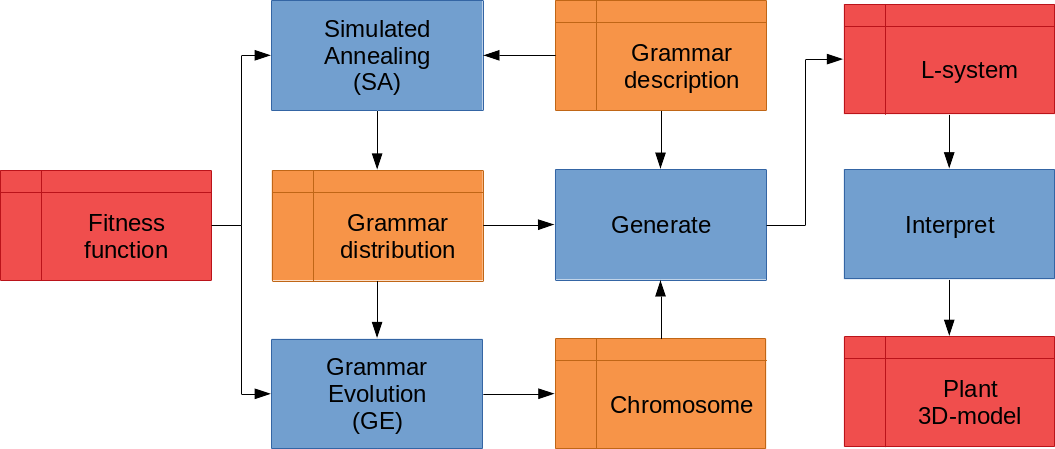
\includegraphics[width=1.0\textwidth]{figures/dgel}
    \caption[DGEL components and flow]{\gls{DGEL} components and flow. Blue boxes represent processes and red boxes represent models. Grey boxes are logical collections of the components.}
    \label{fig:dgel}
\end{figure}

Figure~\ref{fig:dgel} illustrates the modules, processes and models of the \gls{DGEL} algorithm.
It consists of two modules: \textit{Evaluation} and \textit{Generation}.
Evaluation evaluates how good an \gls{L-system} plant is, and the Generation uses this information to generate good \gls{L-system} plants.
The end result is a plant 3D model that is interpreted from an \gls{L-system}.
The \gls{L-system} is generated by a chromosome using a grammar distribution for a grammar description.
These three models: the grammar description, grammar distribution and the chromosome, together define the \gls{L-system}.
All \glspl{L-system} generated using the same grammar description, grammar distribution and chromosome will result in the exact same \gls{L-system}, which also will be interpreted into the exact same plant 3D model.
\gls{GE} is used to generate a good chromosome based on the grammar description, grammar distribution and a fitness function.
The grammar distribution is generated by \gls{SA} based on the grammar description and a fitness function.
The fitness function models how aesthetically pleasing a plant is by assigning it a score in range $[0, 1]$, where 0 is the worst, and 1 is the best.

\section{Representing an L-system with Grammar}
\label{sec:grammar}
As described, the \glspl{L-system} in \gls{DGEL} are represented by a chromosome, a grammar description and a grammar distribution.
If we assume a uniform grammar distribution, only a chromosome and a grammar description is required.

The grammar description, represented in Augmented BNF (ABNF)~\cite{RFC5234}, describes the syntax of the \gls{L-system}.
For example, it may describe that an \gls{L-system} consists of a number of rules, each with a predecessor and successor, where a predecessor contains one character.
The chromosome describes the choices to be made in the grammar description, for example how many rules there are, or which character the predecessor contains.
These choices are what creates the variations in the \glspl{L-system}.
If there were no choices, there would only exist one single \gls{L-system}.

This method of representing the \glspl{L-system} was based on Beaumont and Stepney's work on applying \gls{GE} to plant \glspl{L-system}~\cite{2009Beaumont}, in addition to Ortega et al.'s work on applying it to fractal \glspl{L-system}~\cite{2003Ortega}, and Ryan et al.'s introduction of \gls{GE}~\cite{1998Ryan}.
Though instead of using traditional BNF, ABNF is used because of its support for repetitions with minimum and maximum, grouping and value ranges, and the fact that it has a simpler syntax~\cite{RFC5234}.

While Ortega et al.\ and Beaumont and Stepney make assumptions about the grammar to significantly simplify it and reduce the search space~\cite{2003Ortega, 2009Beaumont}, the \gls{DGEL} method uses a grammar that covers the largest search space reasonably possible.
To make the search space reasonable, there still has to be some limits.
The number of productions, string length, and number of characters for a variable were limited to a maximum of 20.
A higher number did not seem reasonable as no \glspl{L-system} in the literature reviewed used larger numbers, and the search times for higher numbers started to become unreasonably long.
% TODO: "unreasonable" and "Reasonable" are not really clear, or operationally defined. It is OKish, but, you could try to be more precise.
Additionally, to limit the complexity of \glspl{L-system}, complex features such as leaves, flowers, \gls{branch segment} width and more were not included.
Thus the grammar used can only produce the branches of a plant.
This is the most essential part of a plant, which can be expanded later by modifying only the grammar description.
Listing~\ref{lst:grammar} shows the actual grammar description used during the development and testing of the algorithm, while Listing~\ref{lst:grammar2} shows a grammar description that supports leaves and varying \gls{branch segment} width.

\begin{lstlisting}[caption={[ABNF grammar description used in DGEL]{ABNF grammar description used in \gls{DGEL}}}, label=lst:grammar, float]
lsystem = axiom productions
axiom = string
productions = 1*20production
production = predecessor successor
predecessor = variable
successor = string
string = 1*20(symbol / stack)
stack = "[" string "]"
symbol = variable / operation
variable = %x41-55
operation = "+" / "-" / "^" / "&" / ">" / "<"
\end{lstlisting}

\begin{lstlisting}[caption=ABNF grammar description supporting leaves and varying \gls{branch segment} width, label=lst:grammar2, float]
lsystem = axiom productions
axiom = string
productions = 1*20production
production = predecessor successor
predecessor = variable
successor = string
string = 1*20(symbol / stack / leaf)
symbol = variable / operation
variable = %x41-55
operation = "+" / "-" / "^" / "&" / ">" / "<" / "!"
stack = "[" string "]"
leaf = "['{+f-f-f+|+f-f}]"
\end{lstlisting}

To be able to use different grammar distributions, the chromosome representation is a different from that of Ryan et al.\ where each gene is an unsigned 8-bit integer and the choice to be made is the alternative index by the gene modulo the number of alternatives~\cite{1998Ryan}.
Each gene is still represented by an unsigned integer, but it is 32-bit instead of 8-bit, and the interpretation of the integer is different.

A gene in the \gls{DGEL} chromosome can be viewed as an index into the value range of the 32-bit integer.
This value range, from $0$ to $2^{32}$, can be viewed as a line with segments representing each alternative in a rule in the grammar.
In the case of a uniform distribution the segments would be equal in length, while for a different distribution the lengths will differ.
The value of each gene in the chromosome is randomly picked from a uniform distribution, thus making the actual distribution dependent on the grammar distribution.

Figure~\ref{fig:gene} illustrates an example of this process.
A choice is to be made between $C$, $D$, $E$ and $F$ in the rule $A \rightarrow C / D / E / F$.
A chromosome of length 4 containing 4, 3, 0 and 7 is used, and the next gene to be used in the chromosome is the second position, i.e.\ the value 3.
Each gene is a 3-bit unsigned integer, therefore having 8 possible values in range $[0, 8)$.
Since there are four alternatives, and a uniform distribution is used, the 3-bit value range is split into four segments of 2 values.
The gene value 3 maps into the second segment, which maps to the second alternative in the rule, i.e.\ $D$.
This process would then continue with the next gene, 0, on the $D$ rule.

% TODO: what if there were 3 alternatives? How would the 3-bit structure be split uniformly?

\begin{figure}
    \centering
    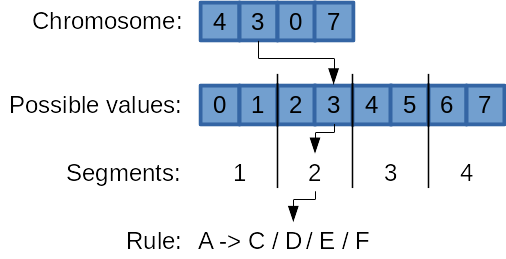
\includegraphics[width=0.8\textwidth]{figures/gene}
    \caption[Example grammar alternative selection from gene]{Example grammar alternative selection from gene. In the figure, the gene is a 3-bit integer, and therefore has 8 possible values.}
    \label{fig:gene}
\end{figure}

\section{Interpreting L-systems Into Plant 3D Models}
\label{sec:interpreting}
As seen in Figure~\ref{fig:dgel}, after an \gls{L-system} has been generated, it needs to be interpreted into a 3D-model such that people may see the plant.
Turtle interpretation is used to do this~\cite{2012Prusinkiewicz}, as it is a popular method used in the literature.y 
% TODO: you use the phrase "... method used in literature." It is a bit weak - methods are really used in research on something, on in application of something, and then described/referred to in literature. So it is a mental shortcut. It would be better, if you spell out exactly where it is used, eg. "Turtle interpretation is a popular method for 2D structure generation based on the L-system." or something along those lines. Check early sections for the use "literature" and see where you can replace it with more accurate/specific formulation.
A 3D version of the turtle interpretation is used, where the turtle can draw lines with \texttt{F}, and rotate around three axes using \texttt{-} and \texttt{+} for yaw, \texttt{\textasciicircum} and \texttt{\&} for pitch, and \texttt{<} and \texttt{>} for roll.
The bracket operators, \texttt{[} and \texttt{]}, are used to create \glspl{branch base}.
Table~\ref{tab:turtle-cmd} shows a complete overview of the characters and their operations, including extra operators used for more control and features like leaves (e.g.\ Listing~\ref{lst:grammar2}).

\begin{table}
    \centering
    \begin{tabular}{| c | l |}
    \hline
    \textbf{Character} & \textbf{Operation} \\ \hline
    F & Draw line forward \\ \hline
    + & Yaw left \\ \hline
    - & Yaw right \\ \hline
    \textasciicircum & Pitch up \\ \hline
    \& & Pitch down \\ \hline
    < & Roll left \\ \hline
    > & Roll right \\ \hline
    | & Yaw 180° \\ \hline
    [ & Push state \\ \hline
    ] & Pop state \\ \hline
    \{ & Begin surface \\ \hline
    \} & End surface \\ \hline
    ! & Decrease width \\ \hline
    ` & Next color \\ \hline
    f & Draw line forward \\
    \hline
    \end{tabular}
    \caption[Turtle interpretation of L-system characters]{Turtle interpretation of \gls{L-system} characters. \texttt{f} does the same as \texttt{F}, but is not allowed as a predecessor int the grammar such that it can not recurse.}
    \label{tab:turtle-cmd}
\end{table}

The actual 3D model created from this interpretation is kept as simple as possible while still trying to look somewhat natural.
The \glspl{branch segment} (created by the \texttt{F} character) are brown stretched cubes.
Leaves are green flat surfaces.
An example can bee seen in Figure~\ref{fig:example-model}.

\begin{figure}
    \centering
    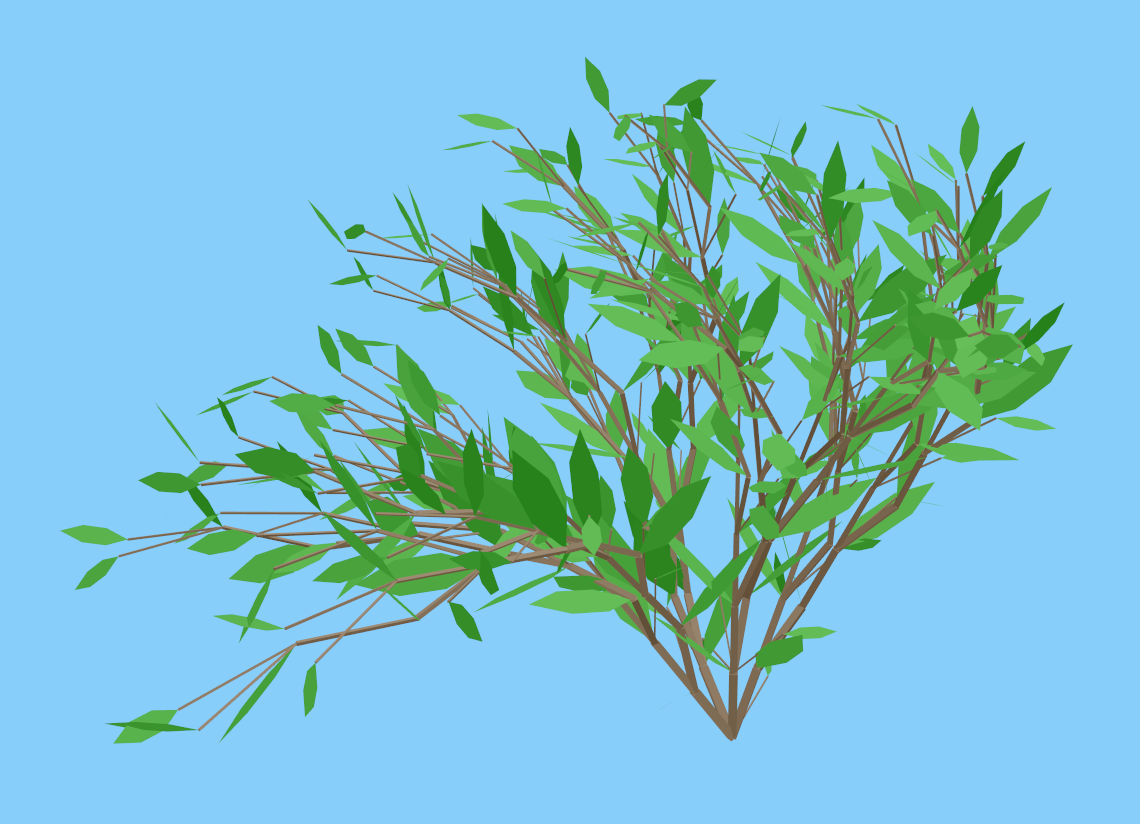
\includegraphics[width=1.0\textwidth]{figures/example-plant}
    \caption[Example 3D plant model generated by DGEL]{Example 3D plant model generated by \gls{DGEL}}
    \label{fig:example-model}
\end{figure}

As a discrete \gls{L-system} is used, the turtle interpretation requires some parameters that control the drawing.
While some evolutionary \gls{L-system} techniques evolve the turtle interpretation parameters as well as the \glspl{L-system}, to keep the process simple, \gls{DGEL} does not.
Additionally, if the discrete \gls{L-system} is swapped with a parametric \gls{L-system}, these parameters are no longer required.
The parameters used here were based on the 3D bush and 3D plant presented by Prusinkiewicz and Lindenmayer (Figures 1.25 and 1.26)~\cite{2012Prusinkiewicz}.
They can be seen in Table~\ref{tab:turtle-param}.

\begin{table}
    \centering
    \begin{tabular}{| l | l |}
    \hline
    \textbf{Parameter} & \textbf{Value} \\ \hline
    Width & 0.05 \\ \hline
    Angle & 22.5° \\ \hline
    Iterations & 5 \\ \hline
    Step & 0.2 \\
    \hline
    \end{tabular}
    \caption{Turtle interpretation parameters}
    \label{tab:turtle-param}
\end{table}

As described earlier, leaves and branches with varying widths are not included.
Without these, the plants may look ``dead'', and so can not be considered very aesthetically pleasing.
To work around this, widths of \glspl{branch segment} were heuristically set and leaves were heuristically placed.
These heuristics were based on observations of real plants and \gls{L-system} based 3D models such as the aforementioned models presented by Prusinkiewicz and Lindenmayer (Figures 1.25 and 1.26)~\cite{2012Prusinkiewicz}.

The \gls{branch segment} widths are determined by their distance from the branch top.
From a branch top, the segment width will increase by a fixed number towards the first \gls{branch base}.
In a \gls{branch base}, the width will be set to the largest of the child \glspl{branch segment}.
Then, the width will continue to increase towards the tree root.
Thus the plant will have natural-looking branches that are larger closer to the root.
Bigger plants will naturally have thicker branches than smaller plants.

Leaves are placed from the branch tops towards the root on each \gls{branch segment} in increasing sizes, until they become too big.
Thus, the leaves on the branch tops are the smallest, and they get bigger towards the root.
To prevent thick \glspl{branch segment}, e.g.\ the trunk of a tree, to have leaves directly placed on them, the leaves will no longer be placed when they reach a certain size.
The leaves are always pitched upwards, with a random noise applied to the pitch to look more natural.
They have a random rotation around the \gls{branch segment} they are placed on.

This interpretation of the \gls{L-system} can be swapped out with a different interpretation, while still using the \gls{DGEL} algorithm.
For example a more realistic interpretation with smoothed branches or branches bent by gravity could be used.
Thus the \gls{DGEL} algorithm is not dependent on this particular interpretation, but the results described later will be.

\section{Using a Grammar Distribution to Limit the Search Space}
In \gls{DGEL}, grammar distributions are used for three reasons: to guide the \gls{GE} to more efficiently find good plants, to guide \gls{GE} to search in a space with certain types of plants, and to prevent infinite recursion.

\begin{figure}
    \centering
    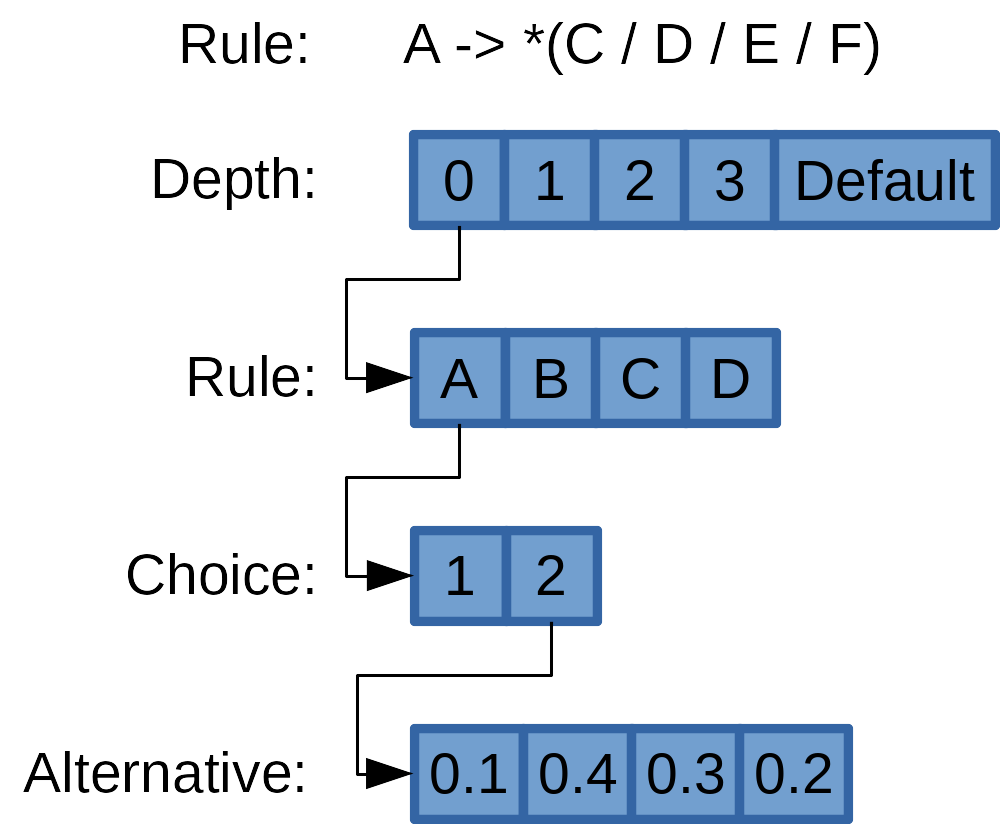
\includegraphics[width=0.6\textwidth]{figures/distribution}
    \caption[Example grammar distribution]{Example grammar distribution applied to the second choice of rule $A$ at depth 0.}
    \label{fig:distribution}
\end{figure}

The distribution is a set of weights per choice per rule per depth, as illustrated in Figure~\ref{fig:distribution}.
The depth is the current branching depth of the \gls{L-system}, controlled by the bracket operators, and defined as the \texttt{stack} rule in the grammar in Listing~\ref{lst:grammar}.

The example figure shows a case where a choice is to be made between the alternatives C, D, E and F in rule $A \rightarrow *(C / D / E / F)$.
There are two different choices in the rule: selecting the number of repetitions (indicated by the asterisk character, \texttt{*}), and selecting the C/D/E/F alternative.
In the example, the depth is 0 (no branching), the rule is $A$ and the choice is the second.
This maps to the weight array: $[0.1, 0.4, 0.3, 0.2]$ which should be applied to the C/D/E/F choice.
Thus, $C$ has a 10\% chance of being selected, $D$ has 40\%, $E$ has 30\%, and $F$ has 20\%.
These weights are then used to define the segments in the gene, as described in Section~\ref{sec:grammar}.

If no weights are found in the distribution for a certain choice at a certain depth, the weights in the ``default'' depth will be used, if they exist.
If not, the weights will be uniform.
This can be used to prevent infinite recursion with the \texttt{stack} rule.
For example, the distribution for the grammar in Listing~\ref{lst:grammar} may specify the weights $[0.5, 0.5]$ for the second choice (\texttt{symbol / stack}) in the \texttt{string} rule at depth 0, 1 and 2, such that there is an equal chance to produce a string and a stack (\gls{branch base}).
To prevent any deeper \glspl{branch base}, the weights $[1.0, 0.0]$ may be specified in the default depth, causing it to not produce a stack at depth 3 or deeper.

By using a specialized distribution, rather than a uniform distribution, the generator may be targeted at specialized \glspl{L-system}, or just have a higher average fitness score for the generated plants.
For example, the distribution may focus more on producing the \texttt{F} character which is used for drawing the \glspl{branch segment}.
Or it may be focused on the \texttt{stack} rule that produces \glspl{branch base}.
This may in turn increase the rate of produced plants that have long or many branches.

In order to find specialized distributions that more efficiently generate good plants or generate different types of plants, the weights in the distribution need to be optimized.
As the distribution maps from depth, to rule, to choice, to alternative (weight), it is a four-dimensional parameter space.
\gls{DGEL} uses \gls{SA} to perform the optimization, but other multi-dimensional parameter optimizers could just as well be used.

Specifically, \gls{DGEL} implements the basic \gls{SA} approach~\cite{2000Ozdamar}, as described by Onbaşoğlu and Özdamar~\cite{2001Onbasoglu}.
The only difference is that the initial solution is not initialized randomly, but initialized from a pre-optimized solution, so that it has a better starting point.
In the \gls{DGEL} \gls{SA}, the \textit{solution} is the distribution itself, filled with weights for each of the alternatives in each of the choices in each of the rules in a limited set of depths.

A neighbor solution is generated in the same manner as Onbaşoğlu and Özdamar describes~\cite{2001Onbasoglu}: selecting one single random weight and either increasing or decreasing the weight randomly, bounded to the range $[0.0, 1.0]$ in the case of \gls{DGEL}.
A key difference is that since these are \textit{weights}, the remaining weights in the same set of weights have to be modified such that the sum of all of the weights equal 1.
If the sum of the remaining weights is greater than 0, they can be scaled by a normalization factor, calculated by $\frac{(1 - w)}{(1 - w_0)}$, where $w$ is the new value of the modified weight, and $w_0$ is the old value of the modified weight.
If the sum of the remaining weights is exactly 0, scaling the weights will not work, as they would remain 0.
The alternative solution is to divide the ``remaining weight'' over the remaining weights.
This is done by setting the remaining weights to $\frac{(1 - w)}{(n - 1)}$, where $w$ is the new value of the modified weight, and $n$ is the number of weights.

Accepting a neighbor solution also follows the same approach as Onbaşoğlu and Özdamar describes~\cite{2001Onbasoglu}.
To do this, an $f(x)$, where $x$ is a grammar distribution, has to be defined.
The performance of a grammar distribution can not directly be measured, but it can be estimated by measuring the average performance of the \glspl{L-system} it generates.
As the performance of the \glspl{L-system} generated may vary by a big degree, the average performance, $mean$, is only accepted after a specified amount of \glspl{L-system}, $n$, have been generated, and the standard error of the performance, $se$, is below a threshold value, $t$ (Algorithm~\ref{alg:eval-dist}).

\begin{algorithm}
\caption{Distribution evaluation}
\label{alg:eval-dist}
\begin{algorithmic}
\Function{evaluate\_dist}{$dist$, $n$, $t$}
    \State $samples\gets \Call{empty\_list}{}$
    \State $mean\gets UNDEFINED$
    \State $se\gets INFINITE$
    \While {$se\geq t$}
        \State $new\_samples\gets \Call{generate}{$n$, $dist$}$
        \State $samples\gets \Call{concat}{$samples$, $new\_samples$}$
        \State $mean\gets \Call{mean}{$samples$}$
        \State $se\gets \Call{standard\_error}{$samples$}$
    \EndWhile
    \State \Return $mean$
\EndFunction
\end{algorithmic}
\end{algorithm}

\section{Using Grammar Evolution to Search the Space}
The main component of \gls{DGEL} is the \gls{GE} of the \glspl{L-system}, which is used to search the parameter space for the best \gls{L-system}.
The \gls{GE} process takes a grammar description and a grammar distribution as the input, and produces a single \gls{L-system} chromosome as the output.

It follows the process as described by Ryan et al.~\cite{1998Ryan}, but with some modifications to the representation as described in Section~\ref{sec:grammar}.
Ryan et al.\ do not describe the selection strategy they used, while Beaumont and Stepney use a simple selection strategy where a percentage of the best individuals are selected as parents~\cite{2009Beaumont}.
Since \gls{GE} is a specialization of \gls{GA}, \gls{GE} can use the same selection strategies as \gls{GA}.
Thus, tournament selection was selected for \gls{DGEL}, based on Blickle and Thiele's structured comparison of selection strategies~\cite{1995Blickle}, and Razali and Geraghty's comparison of selection strategies applied to the traveling salesman problem~\cite{2011Razali}.
Both tournament selection and ranking selection are recommended as good options, but tournament selection performs faster~\cite{1995Blickle}.
Therefore, because it is assumed that \gls{DGEL} may be used in real-time applications, tournament selection is preferred.

In order for the choice of tournament selection based on Blickle and Thiele's comparison to be valid, the \gls{GE} algorithm is implemented as \gls{GA} is described by Blickle and Thiele~\cite{1995Blickle}.
The only difference from the \gls{GA} algorithm is the addition of the duplication and prune operators that were specifically added to \gls{GE} because of their benefits in biology~\cite{1998Ryan}. % TODO: such as ....

\section{Using a Fitness Function to Evaluate Plants}
A crucial component of both the \gls{SA} and \gls{GE} process is the fitness function.
The fitness function is used by \gls{SA} to evaluate the grammar distributions, and by \gls{GE} to evaluate individual \glspl{L-system}.
Its function is to evaluate how ``good'' the \gls{L-system} plants are, or more specifically how ``aesthetically pleasing'' they are.
The literature on evolutionary \glspl{L-system} generally aim the fitness function at evaluating how realistic the plants are by using metrics such as its light gathering ability, positive phototropism and structural stability.

It is assumed that a baseline for aesthetically pleasing plants is that they look at least somewhat realistic, otherwise they would not look like plants at all.
Thus, the metrics used for the fitness function in \gls{DGEL} uses metrics from the literature, or metrics inspired from the literature, where the metrics usually are targeted towards realistic plants.
Additionally, the metrics were improved upon by generating a plants and looking for bad features in well-scored plants.
Following Ochoa~\cite{1998Ochoa}, each metric is weighted so that their importance may be tuned.
Table~\ref{tab:fitness} lists all of the metrics and their weight.

\begin{table}
    \centering
    \begin{tabularx}{\textwidth}{| l | X | l | l |}
    \hline
    \textbf{Metric} & \textbf{Description} & \textbf{Equation} & \textbf{Weight} \\
    \hline
    Nothing & Punish plants that have no branches (can not be seen) & \ref{eq:nothing} & 1 \\
    \hline
    Closeness & Punish plants with child \glspl{branch segment} very close to each other & \ref{eq:closeness} & 1 \\
    \hline
    Drop & Punish plants based on how much the plant grows downwards & \ref{eq:drop} & 1 \\
    \hline
    Balance & Reward plants that have their center of gravity closer to their root & \ref{eq:balance} & 1 \\
    \hline
    Branching & Reward plants with a balanced number of child branches & \ref{eq:complexity} & 1 \\
    \hline
    Foliage & Reward plants with more leaves & \ref{eq:foliage} & 1.5 \\
    \hline
    Length & Reward longer plants & \ref{eq:length} & 1 \\
    \hline
    Curvature & Reward plants that have somewhat curving branches & \ref{eq:curvature} & 0.4 \\
    \hline
    \end{tabularx}
    \caption{Fitness metrics}
    \label{tab:fitness}
\end{table}

\textit{Nothing} is the simplest and most basic metric.
It punishes plants that have no \glspl{branch segment}.
This may happen if for example the \gls{L-system} contains no drawing commands (the character \texttt{F}).
Equation~\ref{eq:nothing} demonstrates this by giving it a score of -1 if it does not have any \glspl{branch segment}.
In this case no other metrics will make any difference.
The $branches$ function returns the number of \glspl{branch segment}.

Because of the recursive property of \glspl{L-system} and the flexible grammar used in \gls{DGEL}, the expanded string from running all the iterations may become very large.
For example, if the axiom contains the letter \texttt{F}, and the production \texttt{F} produces 20 \texttt{F}, with 5 iterations, the expanded string would have length $20^5$.
Additionally, the interpreted 3D model would consist of $20^5 + 1$ points, which is too much for the simple 3D renderer used.
Therefore the number of points in the interpreted 3D model is limited to 10,000 (skeleton limit).
If the \texttt{F} was instead a rotation operator, $20^5$ matrix multiplications would have to be performed, and the skeleton limit would not be breached.
Thus the number of instructions (i.e. characters in expanded string) is limited to a maximum of 50,000 (instruction limit).
Both limits were experimentally found to be balanced in time and space, while still allowing complex structures.
If they are breached the \gls{L-system} will become \textit{nothing} and thus be scored zero
% TODO: a bit confusing that nothing is scored zero but the equation says -1 if no branches.
\begin{equation}
\label{eq:nothing}
    nothing(x) =
    \begin{cases}
        0,& \text{if } branches(x) > 0  \\
        -1,& \text{otherwise}
    \end{cases}
\end{equation}

\textit{Closeness} is another punishing metric that punishes plants that have \glspl{branch base} with \glspl{child segment} too close to each other.
This metric helps avoid plants that have segments clipping into each other.
This clipping may look bad, and if they are completely inside each other the complexity of the 3D model increases, which decreases the rendering performance without improving visuals.
The dot product between the direction of two \glspl{child segment} is used for this metric.
The smaller the angle between the two direction vectors is, the larger the dot product is, becoming 1 when they are parallel.
If the largest dot product between segment directions in a \gls{branch base} is below a threshold, $t$, there is no punishment.
Otherwise, the plant is punished by a factor depending on how much above the threshold the dot product is.
This factor is interpolated between 0 and 1 linearly from the threshold to 1.
Equation~\ref{eq:closeness} shows how the closeness is calculated.
The $closest$ function finds the closest dot product between \glspl{child segment} in a \gls{branch base}.
The threshold was experimentally set to 0.9 to punish plants that have segments that look like they clip into each other.

\begin{equation}
\label{eq:closeness}
    closeness(x) =
    \begin{cases}
        0,& \text{if } closest(x) < t \\
        -\frac{c - t}{(1 - t)},& \text{otherwise}
    \end{cases} \\
\end{equation}

\textit{Drop} is a third punishing metric that punishes plants that grow downwards.
It finds the lowest point on the plant, and punishes the plant if it is below 0.
Equation~\ref{eq:drop} demonstrates this.
The $lowestpoint$ function returns the smallest value of the y-component of all points on the plant.
This value is then clamped in the range -1 and 1 and interpolated using a sine function to quickly increase the punishment.
Thus plants where the lowest point is 0 or above will not be punished, while on plants where it is -1 or below will be punished by -1.

\begin{equation}
\label{eq:drop}
drop(x) = sin(clamp(lowestpoint(x), -1, 0) * \frac{\pi}{2})
\end{equation}

\textit{Balance} is a measure of how well balanced the weight of the plant is.
It is inspired by the Bilateral Symmetry measure by Ochoa where 2D plants that reach equally far both left and right are rewarded the most~\cite{1998Ochoa}.
A different approach has to be taken in 3D where there are not only two horizontal directions, but rather an infinite number.
The approach taken is to estimate where the center of gravity of the plant is, calculate the horizontal distance, $centerdistance$, to it, and compare it to how far the plant reaches, $centerspread$, in the horizontal direction of the center of gravity.
This is done by Equation~\ref{eq:balance}.
In the worst case, if both $centerdistance$ and $centerspread$ are the same, the plant will be punished by -1.
In the best case, if the $centerdistance$ is 0, i.e.\ the gravitational center is in the center of the plant, the plant will be rewarded by 1.
Since $centerdistance$ generally will increase with increasing $centerspread$, the plant will be more punished the more it spreads out in one direction.
Though by having most of its \glspl{branch segment} close to the root, it may mitigate the punishment.
Thus the fraction $\frac{centerdistance}{centerspread}$ is used.

\begin{equation}
\label{eq:balance}
balance(x) = (0.5 - \frac{centerdistance(x)}{centerspread(x)}) * 2
\end{equation}

\textit{Branching} measures how complex the branching of the plant is.
It is inspired by the Structural Stability~\cite{1998Ochoa}, Plant Structural Stability~\cite{2009Corchado} and Proportion of Branch Bases~\cite{1998Ochoa} measures.
These measures assume that the plant becomes too unstable to survive if it has too many \glspl{child segment} growing from a \gls{branch base}.
Corchado et al.\ additionally assume that plants with too few branches will have worse light gathering ability.
Thus there will be a sweet spot in the branching proportion which is rewarded the most.
If the proportion is too low or too high, the plant will be punished.
This is shown in Equation~\ref{eq:complexity} where if the branching proportion is below 1.2 (1.2 \glspl{child segment} from a \gls{branch base} on average), or above 5, it will be punished in range $[-1, 0]$.
While between 1.2 and 5, it will be rewarded in range $[0, 1]$.
The sweet spot is 2, where it will be rewarded by 1.
$icos$ interpolates the value from the first parameter, $a$, to the second parameter, $b$, using a cosine function.
The third parameter, $t$, is in range $[0, 1]$ and controls where between $a$ and $b$ the interpolation is.
This creates a smooth curve between the limits.

\begin{equation}
\label{eq:complexity}
\begin{aligned}
    branching(x) =
    \begin{cases}
        -1, & b < 1 \\
        icos(-1, 0, \frac{b - 1.0}{0.2}), & b < 1.2 \\
        icos(0, 1, \frac{b - 1.2}{0.8}), & b < 2 \\
        1, & b < 3 \\
        icos(1, -1, \frac{b - 3}{5.8}), & b < 7 \\
        -1, & \text{otherwise}
    \end{cases}, \\
    \text{where } b = \frac{branches(x)}{branchings(x)}
\end{aligned}
\end{equation}

\textit{Foliage} measures how many leaves a plant has.
It is the main metric for measuring the light gathering ability of the plant, and is inspired by Ochoa~\cite{1998Ochoa}, Ebner~\cite{2003Ebner}, and Corchado et al.'s~\cite{2009Corchado} light gathering ability metrics.
The main point is that more leaves exposed to sunlight means that the plant has a better ability to survive.
For simplicity, the metric used in \gls{DGEL} is based on Corchado et al.'s metric which simply rewards plants with more leaves~\cite{2009Corchado}.
It also counts leaves that are shadowed by other leaves, even though in reality these would gather only minimal amounts of light.
This selection of method was due to time constraints, and a more complex method like Ebner's would be better.
The metric used starts with a reward of 0 for 0 leaves and is asymptotic towards 1 when the leaf count, found by $leaves$, increases towards $\infty$.
Equation~\ref{eq:foliage} demonstrates this.
The $s$ constant controls how fast it should increase towards 1.

\begin{equation}
\label{eq:foliage}
    foliage(x) = \frac{leaves(x) * s}{1 + leaves(x) * s}, \text{where } s = 0.1
\end{equation}

\textit{Length} rewards plants that are longer.
It is inspired by Ochoa and Corchado et al.'s Positive Phototropism metrics where the assumption is that plants grow towards the sunlight and therefore taller plants are better at surviving.
While Positive Phototropism only cares about the height of the plant, Length cares about how long the plant is, not considering if it grows upwards or not.
This change is made on the assumption that plants can gather more light both by growing upwards (cover more vertical area) and sideways (cover more horizontal area).
Additionally it was found during an early experiment that short plants were generally displeasing.
Like the Foliage metric, the Length metric is asymptotic towards 1 as the plant length increases towards $\infty$.
This is shown in Equation~\ref{eq:length}.
The length of the plant is found using $longest$, which finds the longest path in the branches of the plant from root to leaf and returns the number of \glspl{branch segment} in it.
As with the Foliage metric, the $s$ constant controls how fast it should increase towards 1.

\begin{equation}
\label{eq:length}
    length(x) = \frac{longest(x) * s}{1 + length(x) * s}, \text{where } s = 0.5
\end{equation}

\textit{Curvature} is a metric that rewards plants with more curved branches.
It was developed from the results of the first experiment where it was found that plants that looked ``static'' or ``straight'' were not as pleasing as plants that looked more ``dynamic'' or ``curvy''.
As Equation~\ref{eq:curvature} demonstrates, the plant is rewarded more if the \glspl{branch segment} are oriented with a small angle different from their parent.
If the angle is too sharp, the plant is rewarded less, as the plant may look like ``doodles'' with such angles.
The $minangles$ function returns a list of the smallest angle from an \gls{internode segment} to its parent segments.
Thus, if an \gls{internode segment} only has one child (i.e.\ it does not branch), the smallest angle will be the angle between it and that one child.
Otherwise, if an \gls{internode segment} has multiple children (i.e.\ it is a \gls{branch base}), all of the angles between it and the children are calculated and the smallest will be used.
This is based on the assumption that the \gls{child segment} with the smallest angle is the \gls{straight segment} following a \gls{branch base}.
% This assumption only holds for apex trees? What if it branches into two equally angled branches?
$avg$ calculates the average of all of the angles returned by $minangles$.
Like in Equation~\ref{eq:complexity}, $icos$ is used to create a smooth interpolation between the limits $min$, $opt$ and $max$.
A sweet spot of $opt = 0.24711092$, which is rewarded by 1, was found to provide a good curvature in the plant.
A limit of $max = \frac{\pi}{4}$ (45°) was intuitively chosen as a point where the curvature is no longer rewarding.

\begin{equation}
\label{eq:curvature}
\begin{aligned}
    curvature(x) =
    \begin{cases}
        icos(0, 1, \frac{a - min}{opt - min}), & a >= min \text{ and } a < opt \\
        icos(1, 0, \frac{a - opt}{max - opt}), & a >= opt \text{ and } a < max \\
        min, & \text{otherwise}
    \end{cases}, \\
    \text{where } a = avg(minangles(x)), \\
    min = 0, \\
    opt = 0.24711092, \\
    max = \frac{\pi}{4} \\
\end{aligned}
\end{equation}

% !TEX root = ../Masters.tex
\chapter{Implementation of DGEL}

% !TEX root = ../Masters.tex
\chapter[Evaluation of DGEL]{Evaluation of \gls{DGEL}}
\gls{DGEL} consists of two main modules: \textit{generation} and \textit{evaluation}.
The evaluation module consists of the fitness component which evaluates how good the \gls{L-system} plants are.
The remaining components are part of the generation component which generates plants, and uses the evaluation module to generate \textit{good} plants.
To answer if \gls{DGEL} solves the research questions, both modules have to be evaluated.
The generation module is evaluated in a technical manner to determine if it performs well or not.
The evaluation module is evaluated using humans as to answer if the fitness function properly rates plants as aesthetically pleasing or not.

\section{Evaluation of the Generation Module}
\subsection{Method}
As explained in Section~\ref{sec:overview} and shown in Figure~\ref{fig:dgel}, there are two main processes involved in generating the model for the \gls{L-system} plants: \textit{\gls{SA}} and \textit{\gls{GE}}.
The remaining steps are dependent on the model and do not create variations on the same model.
Thus \gls{GE} and \gls{SA} are the two processes of interests to evaluate.

While the resulting fitness scores do not depend on the hardware the experiment runs on, the duration used on calculating them does.
It ran on a water-cooled Intel i7-4790K CPU (8M Cache, up to 4.40 GHz)\footnote{Intel i7-4790K: \url{https://ark.intel.com/products/80807/Intel-Core-i7-4790K-Processor-8M-Cache-up-to-4_40-GHz}} with 8GB of RAM.
The \gls{GE}, \gls{SA} and brute-force processes are parallelized and ran with 9 threads.

% Could explain why...
When sample groups are compared, their distributions are tested for normality using the Shapiro-Wilk normality test~\cite{1965Shapiro}.
If Shapiro-Wilk is not applicable because of the sample size, a Q-Q plot is analyzed~\cite{1968Wilk}.
Robust Brown-Forsythe Levene-type test is used to test if the variances in the distributions are equal~\cite{1974Brown}.
Finally, in the cases when normality cannot be assumed, Mann-Whitney U test is used to test the location shift of the distributions~\cite{1947Mann}.

% GE SA vs GE uniform - need data, how to measure?

\subsubsection{Grammar Evolution Parameters}
\gls{GE}, as with \gls{GA}, depends on multiple parameters, and with tournament sampling there are even more.
Therefore, before evaluation the \gls{GE} process, good parameters should be found.
Additionally, seeing what parameters are needed for a good performing \gls{GE} may reveal additional properties of it.
The parameters were found using a combined manual and automated approach by searching the parameter space in multiple steps.
The idea was not to find the optimal parameters, but rather to find some parameters that made the \gls{GE} produce an individual with good fitness within a reasonable time.
It was assumed that the size parameters --- population size and number of generations --- are the baseline parameters for \gls{GE} and thus should be found first.
Then the tournament size for the tournament selection strategy should be found.
Then good parameters for the recombination rates --- crossover rate and mutation rate --- should be found.
Finally the parameter for the \gls{GE} gene duplication operator should be found.
% Reason for these assumptions?

To search for the \gls{GE} parameters, a breadth-first graph search inspired approach was used.
An example is shown in Figure~\ref{fig:parameter-search}.
The approach tests a combination of parameters by doing 20 \gls{GE} runs with those parameters and using the mean fitness score of the best individual from each run.
If the score is an improvement of the previous score, the node is considered an improvement and it will consider the neighboring nodes in the graph by increasing the parameter values.
Otherwise, the current parameter values are considered as not improving the performance and thus be discarded.
When there are no more improvements, the parameter values that produced the best score is returned.
The parameter values start at a small value and increase in an exponential fashion.
This is based on the assumption that the parameters are more sensitive when the values are small.
All of the parameter searches, except for the reproduction parameter and duplication rate search, are increasing with a multiplicative of 2.
Because the reproduction and duplication rate parameters are bounded ($[0, 1]$) and to cover the whole range with a reasonable amount of steps, custom steps of 0.01, 0.1, 0.5 and 1 are used.

\begin{figure}
    \centering
    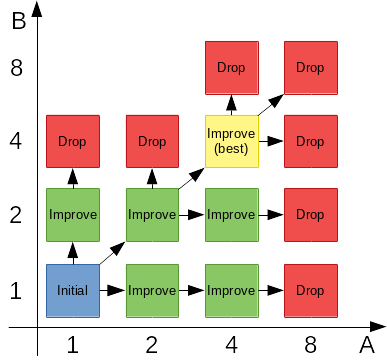
\includegraphics[width=0.6\textwidth]{figures/parameter-search}
    \caption[Example of a GE parameter search]{Example of a \gls{GE} parameter search}
    \label{fig:parameter-search}
\end{figure}

\subsubsection{Grammar Evolution Test}
The reason for using \gls{GE} is to search the space in an efficient way.
To see if it is doing this, it needs to be compared to a brute-force approach that finds completely random samples in the space and picks the best of them.
Thus, the hypothesis is that \gls{DGEL} \gls{GE} finds plants with better fitness scores than brute-force does (\textbf{H1}).

To make a fair comparison, the brute-force should generate as many individuals as the \gls{GE} generates and modifies (through mutation or crossover).
This way, both methods ``generate'' the same amount of individuals, either being completely new individuals or modifications of existing individuals.
\gls{GE} uses a fixed number of generations and population size, resulting into a fixed number of total individuals: $individuals = population + population * generations$, that the brute-force method also generates.

Because both methods depend on a random seed, an average of multiple runs is used.
A sample size of 11 was selected as balanced choice between sample size and duration.

\subsubsection{Simulated Annealing}
% \begin{itemize}
% 	\item Can SA and the grammar distribution be used to find portions of the arameter space that generate better L-system plants?
% 	\item Does SA enable GE to find better L-system plants?
% 	\item Can SA find multiple portions of the parameter space that each generate unique-looking plants?
% \end{itemize}
The main purpose of using \gls{SA} with a grammar distribution is to improve the efficiency of the remaining components of \gls{DGEL} by focusing the search space on a good area.
Based on this a hypothesis can be formulated: An \gls{SA}-optimized grammar distribution can find better individuals than a uniform grammar distribution (\textbf{H2}).
An important word in the hypothesis is \textit{can}, because this means that the hypothesis does not imply that \textit{all} \gls{SA}-optimized grammar distributions find better individuals.

\gls{SA} is used as described in previous sections to find an optimized grammar distribution, and the progress of it is plotted to see if it makes any meaningful progress.
Then, to test the hypothesis a comparison is made between the average fitness of \glspl{L-system} randomly generated by a uniform grammar distribution and \glspl{L-system} randomly generated by an \gls{SA}-optimized grammar distribution.
The \glspl{L-system} are generated in a brute-force manner, not using any evolutionary approach such as \gls{GE}.

% If \textbf{H2} is supported, we can further hypothesize that \textit{\gls{GE}} with an \gls{SA}-optimized grammar distribution can find better individuals than with a uniform grammar distribution (\textbf{H3}).
% Have run tests with 160800 individuals, but \gls{GE} with uniform is already so good that it isn't comparable.
% Thus we need a better comparison (fewer individuals? Time to convergence?)
%To test this hypothesis, the performance of \gls{GE} with a uniform grammar distribution is compared to the performance of \gls{GE} with an \gls{SA}-optimized grammar distribution.
%Both \gls{GE} processes were run 11 times, each time extracting the best L-system, before taking the mean of the best \glspl{L-system} and using a t-test to test if the means were different.

% Finally,check variation of \gls{SA}. How to? Right now I can only manually check some examples.

\subsection{Results}
\subsubsection{Grammar Evolution Parameters}
\begin{figure}
    \centering
    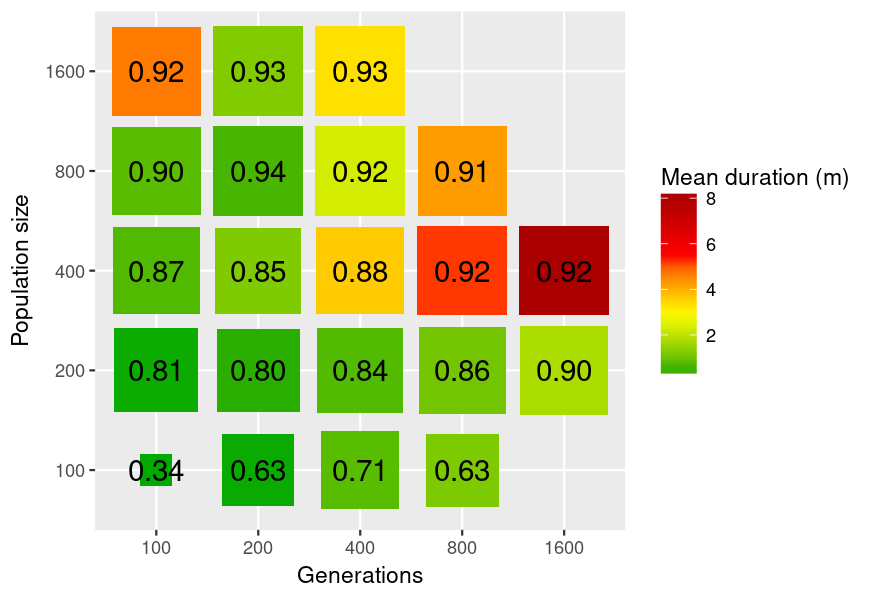
\includegraphics[width=0.8\textwidth]{figures/ge-size-sampling}
    \caption[Visualized search of GE population size and number of generations]{Visualized search of \gls{GE} population size and number of generations. Numbers are the mean of best fitness scores, box sizes are a representation of that number, and colors represent the mean duration of the \gls{GE}.}
    \label{fig:size-sampling}
\end{figure}

Figure~\ref{fig:size-sampling} shows the search of the population size and number of generations to be used for the \gls{GE} process.
The search was prematurely stopped because when either the number of generations or population size reached 1600 the duration became unreasonable long.
As seen, a minimum of either a population size of 200 or 200 generations is required for a reasonable performance.
Additionally, for any number of generations, a population size of 200 makes a notable improvement.
From this point on, there is a steady improvement from scores around 0.8 to 0.9 with both parameters increasing towards 1600.
% Actually draw this line?
Outside a line drawn through 800, 400 and 400, 800 there does not seem to be any notable improvement, while the duration increases by a large amount.
The parameter values that yielded the best fitness was $generations = 200$ and $population size = 800$, and they did it within a reasonable duration.
The duration of it is significantly smaller than other parameter values that yield approximately the same fitness.
Thus these parameter values were selected for use.

\begin{figure}
    \centering
    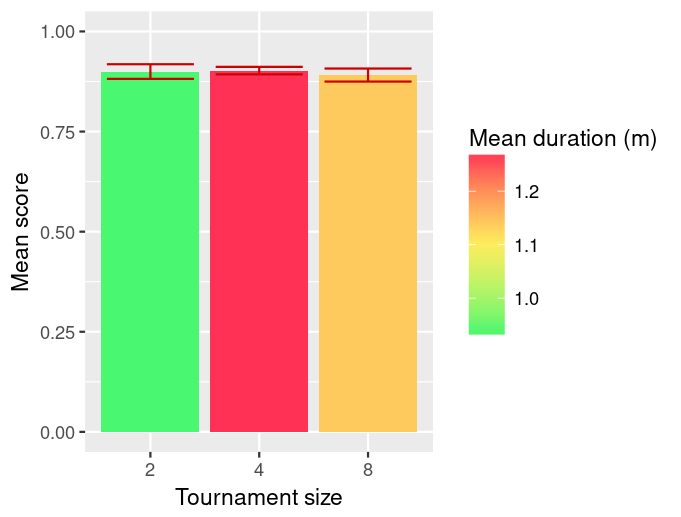
\includegraphics[width=0.7\textwidth]{figures/ge-tournament-sampling}
    \caption[Visualized search of the GE tournament selection tournament size]{Visualized search of the \gls{GE} tournament selection tournament size with standard error}
    \label{fig:tournament-sampling}
\end{figure}

Figure~\ref{fig:tournament-sampling} shows the search of the tournament size.
Contrasted to the other searches, this is a one-dimensional search.
% Possibly do a significance test. Need to re-run to generate raw data...
As seen in the figure, the search did not find any improvements at all.
Therefore the tournament size was kept at the lowest value, i.e.\ 2.

\begin{figure}
    \centering
    \begin{subfigure}{0.57\textwidth}
        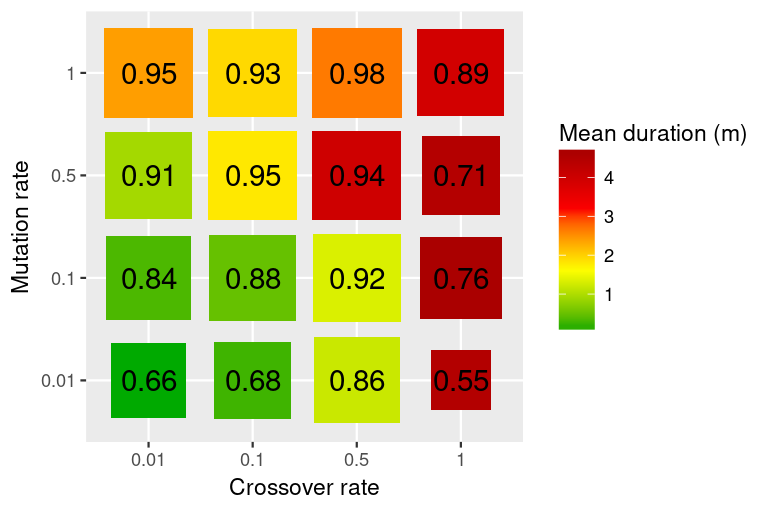
\includegraphics[width=\textwidth]{figures/ge-recombination-sampling}
        \caption{Mean of best fitness scores as numbers and sizes, with duration as colors}
        \label{fig:recombination-sampling}
    \end{subfigure}
    ~
    \begin{subfigure}{0.4\textwidth}
        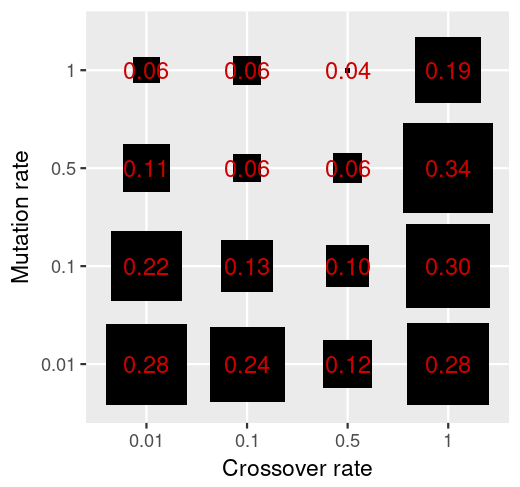
\includegraphics[width=\textwidth]{figures/ge-recombination-sampling-variance}
        \caption{Standard deviation}
        \label{fig:recombination-sampling-variance}
    \end{subfigure}
    \caption[Visualized search of the GE recombination parameters]{Visualized search of the \gls{GE} recombination parameters}
\end{figure}

Figure~\ref{fig:recombination-sampling} shows the search of the recombination parameters: mutation rate and crossover rate.
There is a general improvement in fitness with both increasing mutation rate and crossover rate until the crossover rate reaches 1 where it suddenly turns for the worse.
Therefore the crossover rate should at least be below 1.
Additionally, the crossover rate seems to be the parameter that contributes the least to an improved fitness and increases the duration the most.
Therefore the mutation rate should be the most important parameter.
The best fitness score is provided by a mutation rate of 1 and crossover rate of 0.5, further indicating this.

% Also did an ANOVA on this, could mention.
Figure~\ref{fig:recombination-sampling-variance} shows the standard deviations in the same search.
The pattern is similar to that of the mean fitness scores.
The most stable performance is provided by a mutation rate of 1 and crossover rate of 0.5.
Thus the recombination parameters is set to these values.

\begin{figure}
    \centering
    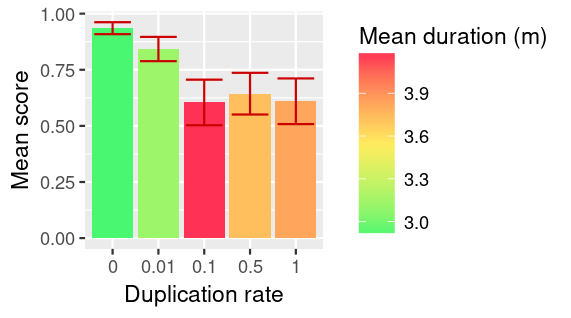
\includegraphics[width=0.7\textwidth]{figures/ge-duplication-sampling}
    \caption[Visualized search of the GE duplication rate]{Visualized search of the \gls{GE} duplication rate with standard error}
    \label{fig:duplication-sampling}
\end{figure}

Figure~\ref{fig:duplication-sampling} shows the search of the duplication rate.
It shows a worsening of both score and duration from a rate of 0 to 0.1, from where it stays bad.
% possibly run anova, but don't have raw data...
Therefore the duplication rate is set to 0.

All of the \gls{GE} parameters are summarized in Table~\ref{tab:ge-parameters}.

\begin{table}
    \centering
    \begin{tabular}{| l | l |}
    \hline
    \textbf{Parameter} & \textbf{Value} \\ \hline
    Population size & 800 \\
    \hline
    Generations & 200 \\
    \hline
    Tournament size & 2 \\
    \hline
    Mutation rate & 1.0 \\
    \hline
    Crossover rate & 0.5 \\
    \hline
    Duplication rate & 0 \\
    \hline
    \end{tabular}
    \caption[GE parameter values selected based on searches]{\gls{GE} parameter values selected based on searches}
    \label{tab:ge-parameters}
\end{table}

\subsubsection{Grammar Evolution Test}
\begin{figure}
    \centering
    \begin{subfigure}{0.4\textwidth}
        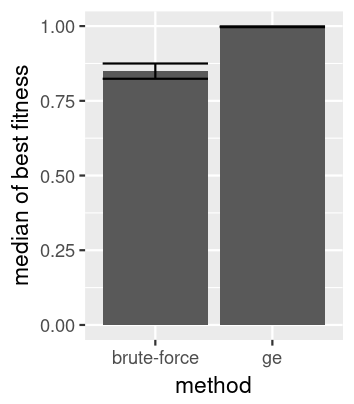
\includegraphics[width=\textwidth]{figures/ge-random}
        \caption{Median of best fitness with MAD}
        \label{fig:ge-random}
    \end{subfigure}
    ~
    \begin{subfigure}{0.4\textwidth}
        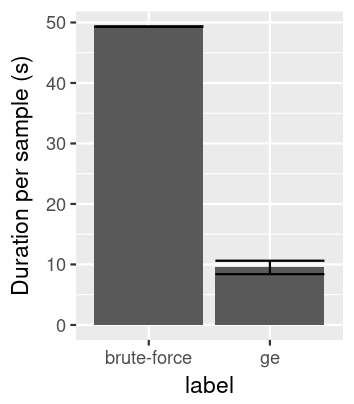
\includegraphics[width=\textwidth]{figures/ge-random-duration}
        \caption{Mean duration with SE}
        \label{fig:ge-random-duration}
    \end{subfigure}
    \caption[GE and random performance compared]{\gls{GE} and random performance compared}
\end{figure}

Figure~\ref{fig:ge-random} shows the comparison of \gls{GE} against random samples.
A Shapiro-Wilk normality test suggests that the brute-force sample distribution can be assumed to be normally distributed (p >= 0.05, W = 0.97), while the \gls{GE} sample distribution can not (p < 0.05, W = 0.46).
A robust Brown-Forsythe Levene-type test suggests that the variances of the distributions can be considered equal (p >= 0.05, statistic = 0.09).
Because there are non-normal distributions and different variances, the Mann-Whitney U test is used.
\gls{GE} has a median score of 1.00, while random has 0.85 (difference of 0.15).
The Mann–Whitney U test suggests that the true location shift of the distributions is greater than 0 (p < 0.05, U = 117).
% Could run test on this as well, but necessary??
% Mariusz: i think not necessary.

Additionally, Figure~\ref{fig:ge-random-duration} shows the mean duration of the methods where \gls{GE} is about 5 times faster than random.
A Shapiro-Wilk normality test suggests that both the brute-force and \gls{GE} samples can be assumed to be normally distributed (p >= 0.05, W = 0.89 and p >= 0.05, W = 0.93 respectively).
A robust Brown-Forsythe Levene-type test suggests that the variances of the distributions can be considered unequal (p < 0.05, statistic = 17.13).
Because the distributions can be assumed to be normally distributed and the variances can be assumed to be unequal, the Welch's t-test is used.
\gls{GE} has a mean duration of 9.51, while random has 49.33 (difference of -39.82).
The Welch's two-sample t-test suggests that the true difference in means are not 0 (p < 0.05, t = -35.90, df = 10.02)

\subsubsection{Simulated Annealing}
\begin{figure}
    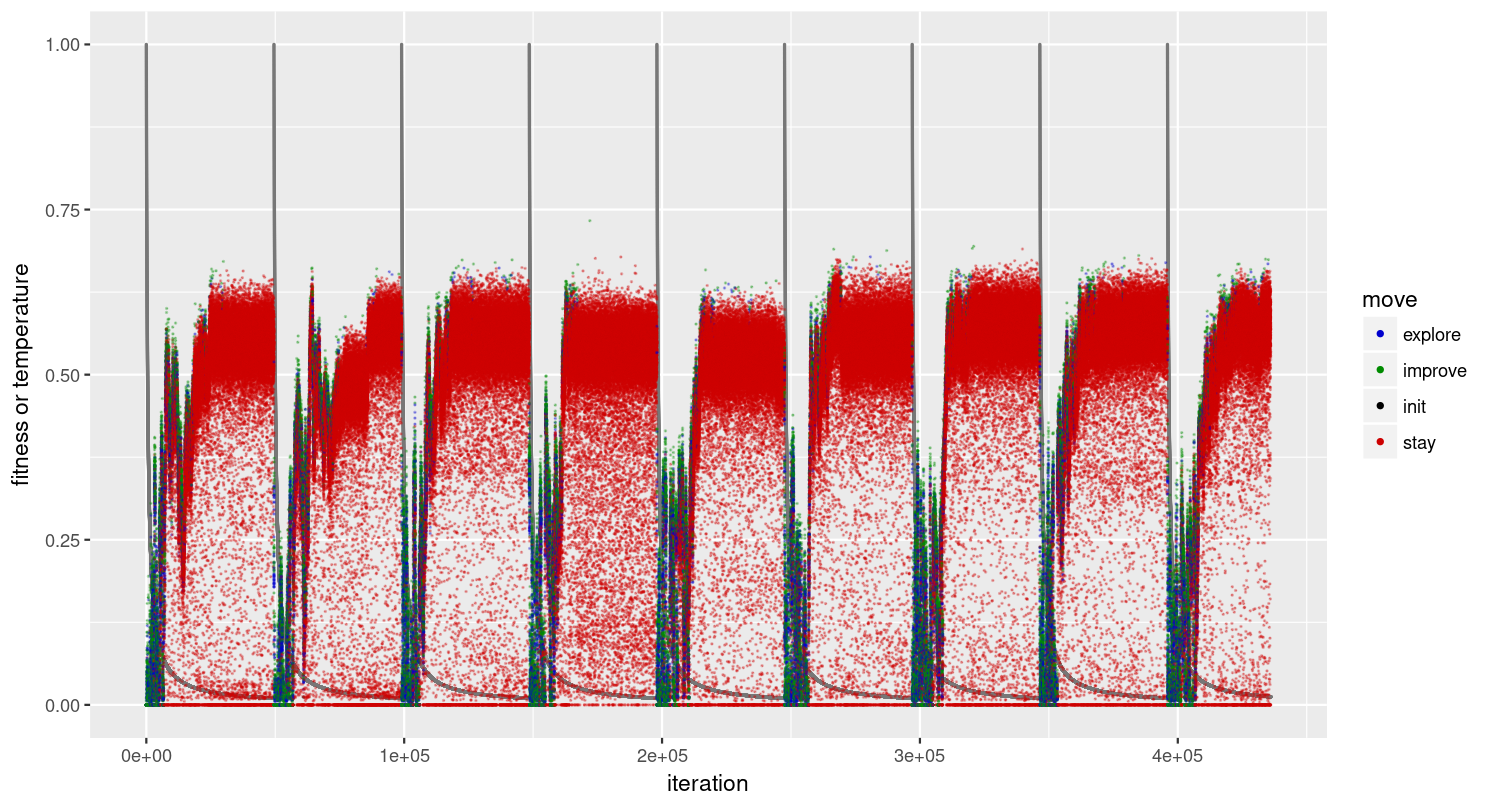
\includegraphics[width=\textwidth]{figures/sa-progress}
    \caption[The complete SA process with multiple re-annealings]{The complete \gls{SA} process with multiple re-annealings}
    \label{fig:sa-progress}
\end{figure}

Figure~\ref{fig:sa-progress} shows the progress of one \gls{SA} run, and Figure~\ref{fig:sa-progress-close} shows a close-up of the first annealing.
The run had a maximum of 2000 moves per dimension and a cooldown rate of 0.002.
The grammar distribution evaluation had a minimum 32 samples and an error threshold of 0.004.
In total this resulted into 436000 moves over 9 annealings.
As seen in the figure, for each annealing there is a general improvement from a fitness score of 0 to around 0.6.
The \gls{SA} process explores the space in the beginning, moving both up and down in score, and then gradually focuses more on hill climbing towards the end.
Each annealing generally reach a plateau before getting halfway through the annealing process, from which point nearly all mutations are worse and so it chooses to stay, though the second annealing is slower to reach the plateau.
The fourth annealing found one exceptionally good grammar distribution with a score of almost 0.75, but when the same grammar distribution was measured over 100000 samples its score was 0.61 (SD = 0.25).
Therefore the score measured in the \gls{SA} process may have been inaccurate.
As this distribution was the one with the best score during the \gls{SA} process, it is the one used for further analysis.

\begin{figure}
    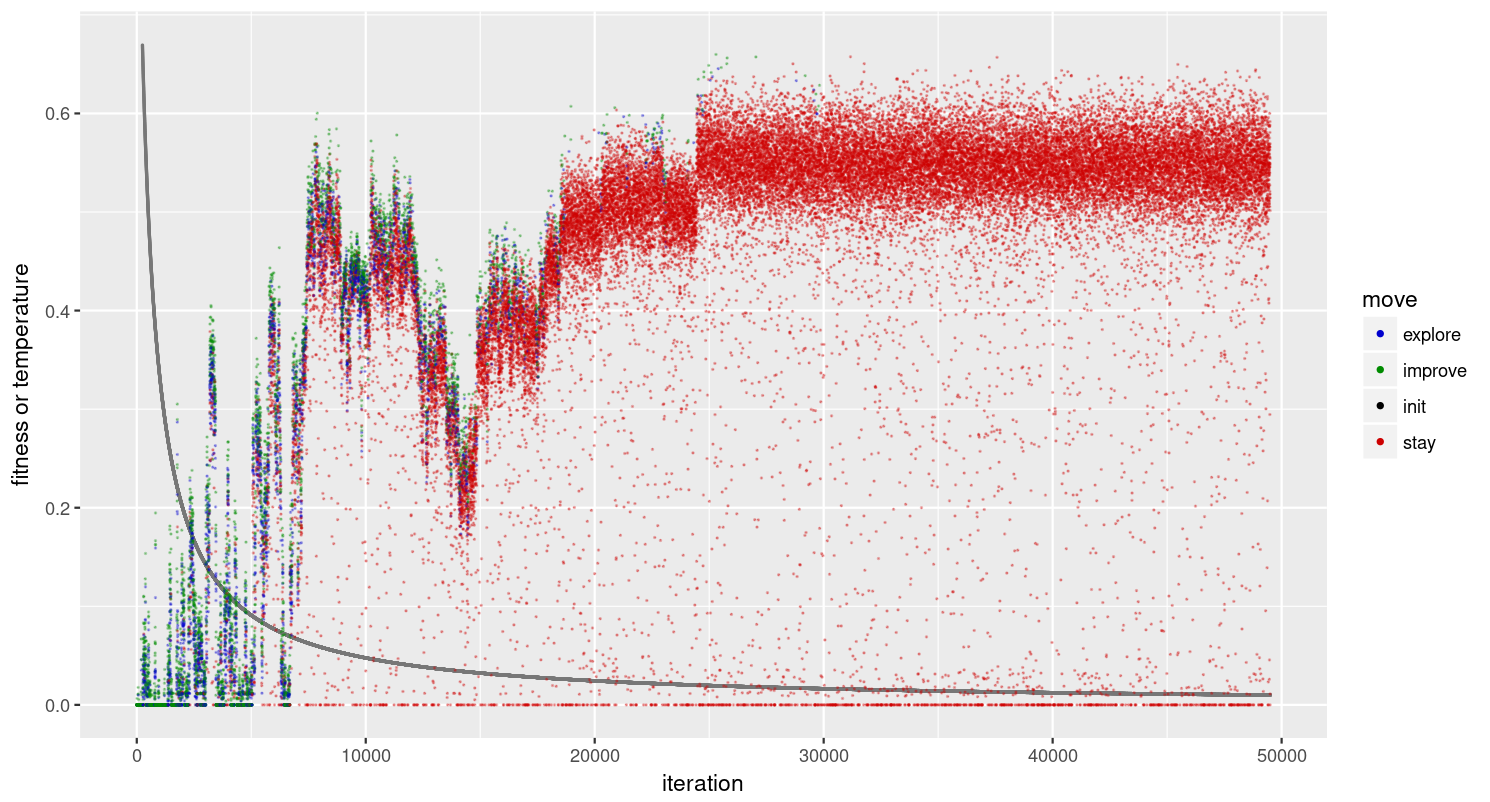
\includegraphics[width=\textwidth]{figures/sa-progress-close}
    \caption[Close-up of the first annealing of the SA process]{Close-up of the first annealing of the \gls{SA} process}
    \label{fig:sa-progress-close}
\end{figure}

Seen in Figure~\ref{fig:sa-progress-close} the points cluster around the same score.
At the same time there are some points spread fairly uniformly between the clustering and 0.
Additionally there is a clustering at exactly 0.

\begin{figure}
    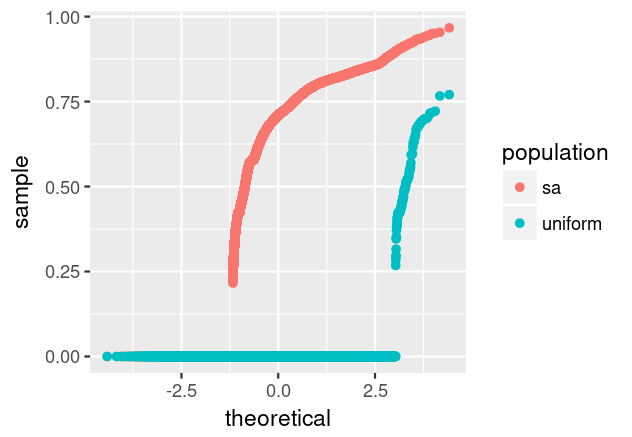
\includegraphics[width=\textwidth]{figures/sa-qq}
    \caption[Q-Q plot of SA and uniform sample populations]{Q-Q plot of \gls{SA} and uniform sample populations}
    \label{fig:sa-qq}
\end{figure}

As the sample size (n = 100000) is too large for a Shapiro-Wilk normality test, a Q-Q plot is used.
It can be seen in Figure~\ref{fig:sa-qq}, and it is clear that the distributions are not normally distributed.
Even with all 0 scores removed, the data does not appear normally distributed.
A robust Brown-Forsythe Levene-type test shows that the variances of the distributions can not be considered equal (p < 0.05).

\begin{figure}
    \centering
    \begin{subfigure}{0.48\textwidth}
        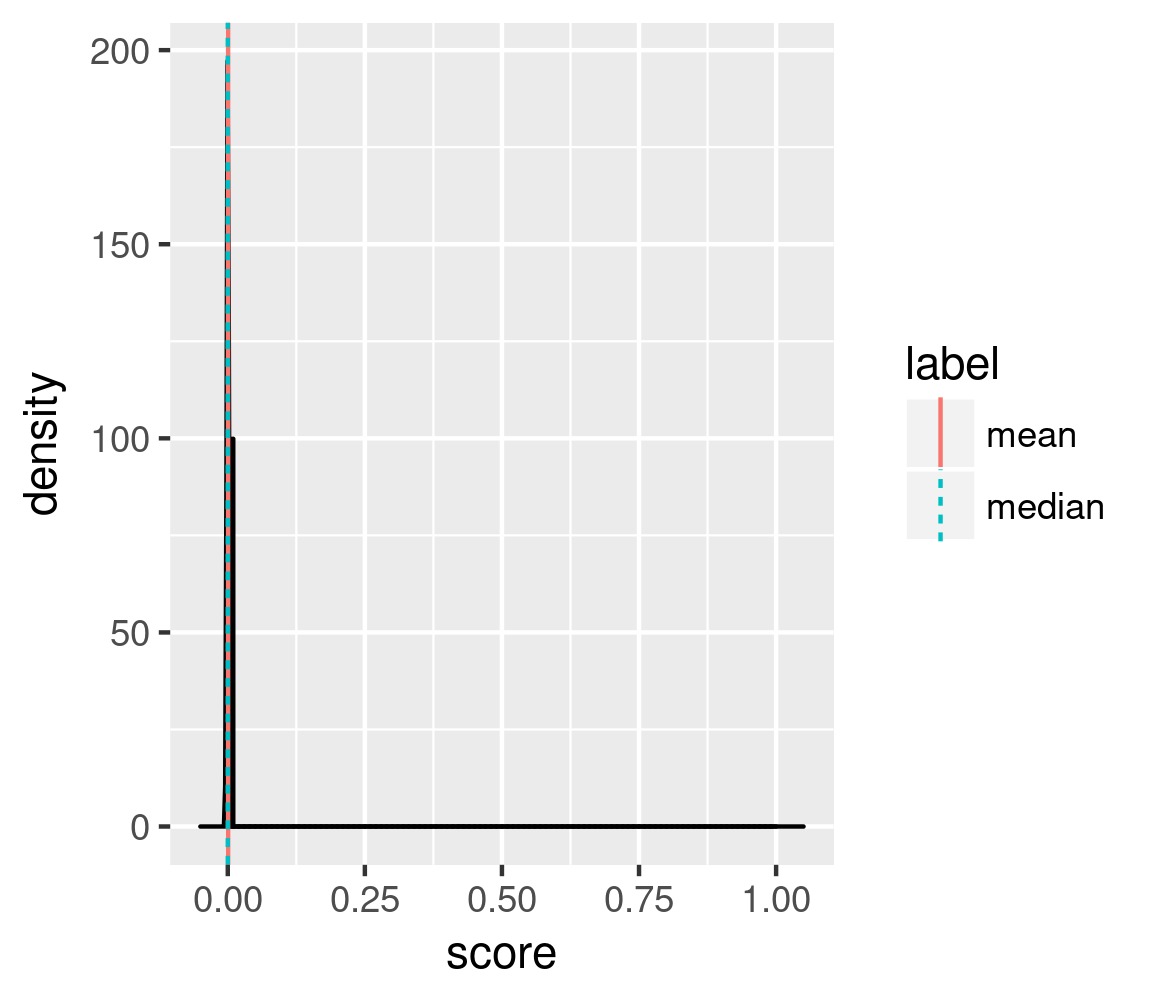
\includegraphics[width=\textwidth]{figures/uniform-population}
        \caption{Complete sample population}
        \label{fig:uniform-population}
    \end{subfigure}
    ~
    \begin{subfigure}{0.48\textwidth}
        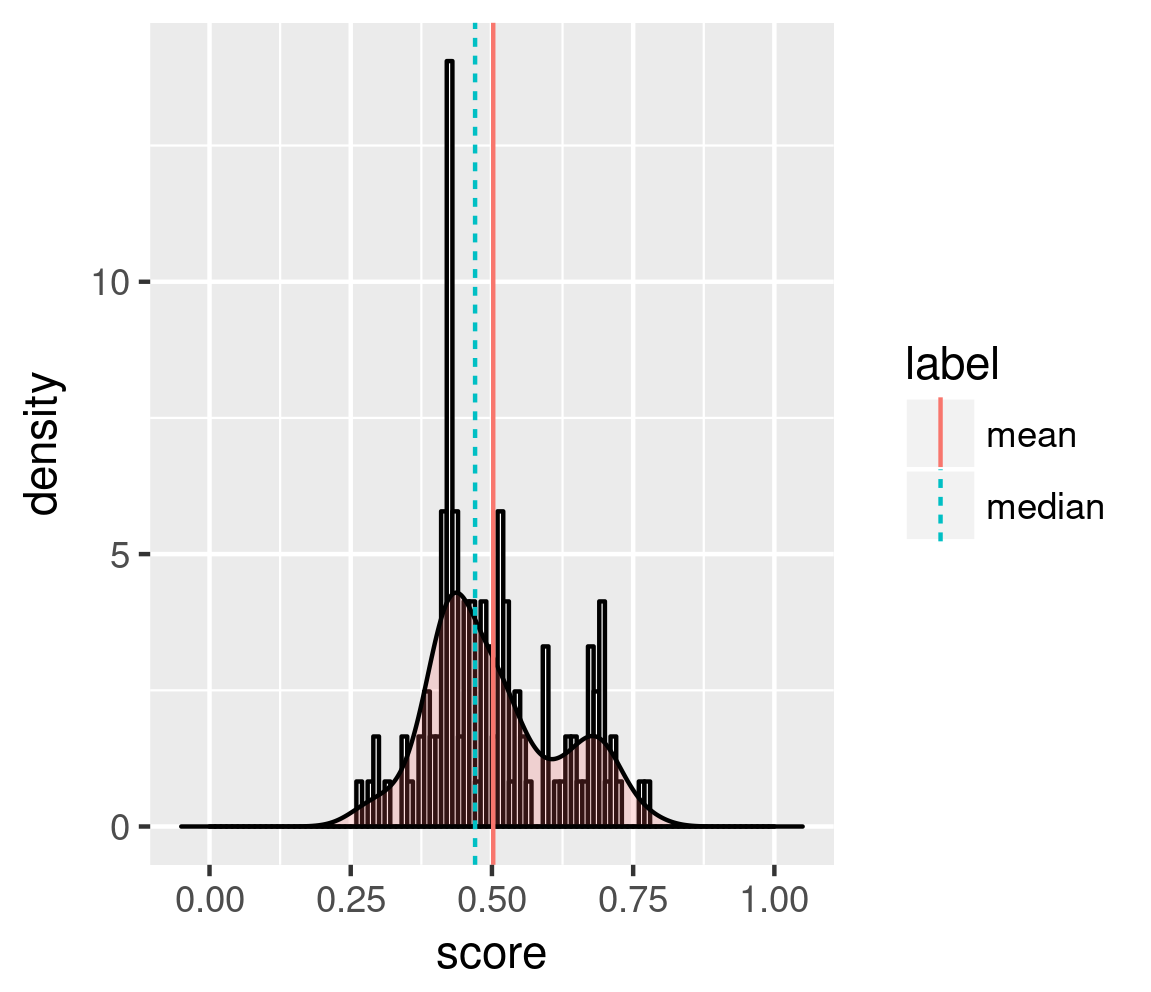
\includegraphics[width=\textwidth]{figures/uniform-population-no0}
        \caption{Sample population without samples with score 0}
        \label{fig:uniform-population-no0}
    \end{subfigure}
    \caption{Sample population of L-systems generated using a uniform grammar distribution}
\end{figure}

\begin{figure}
    \centering
    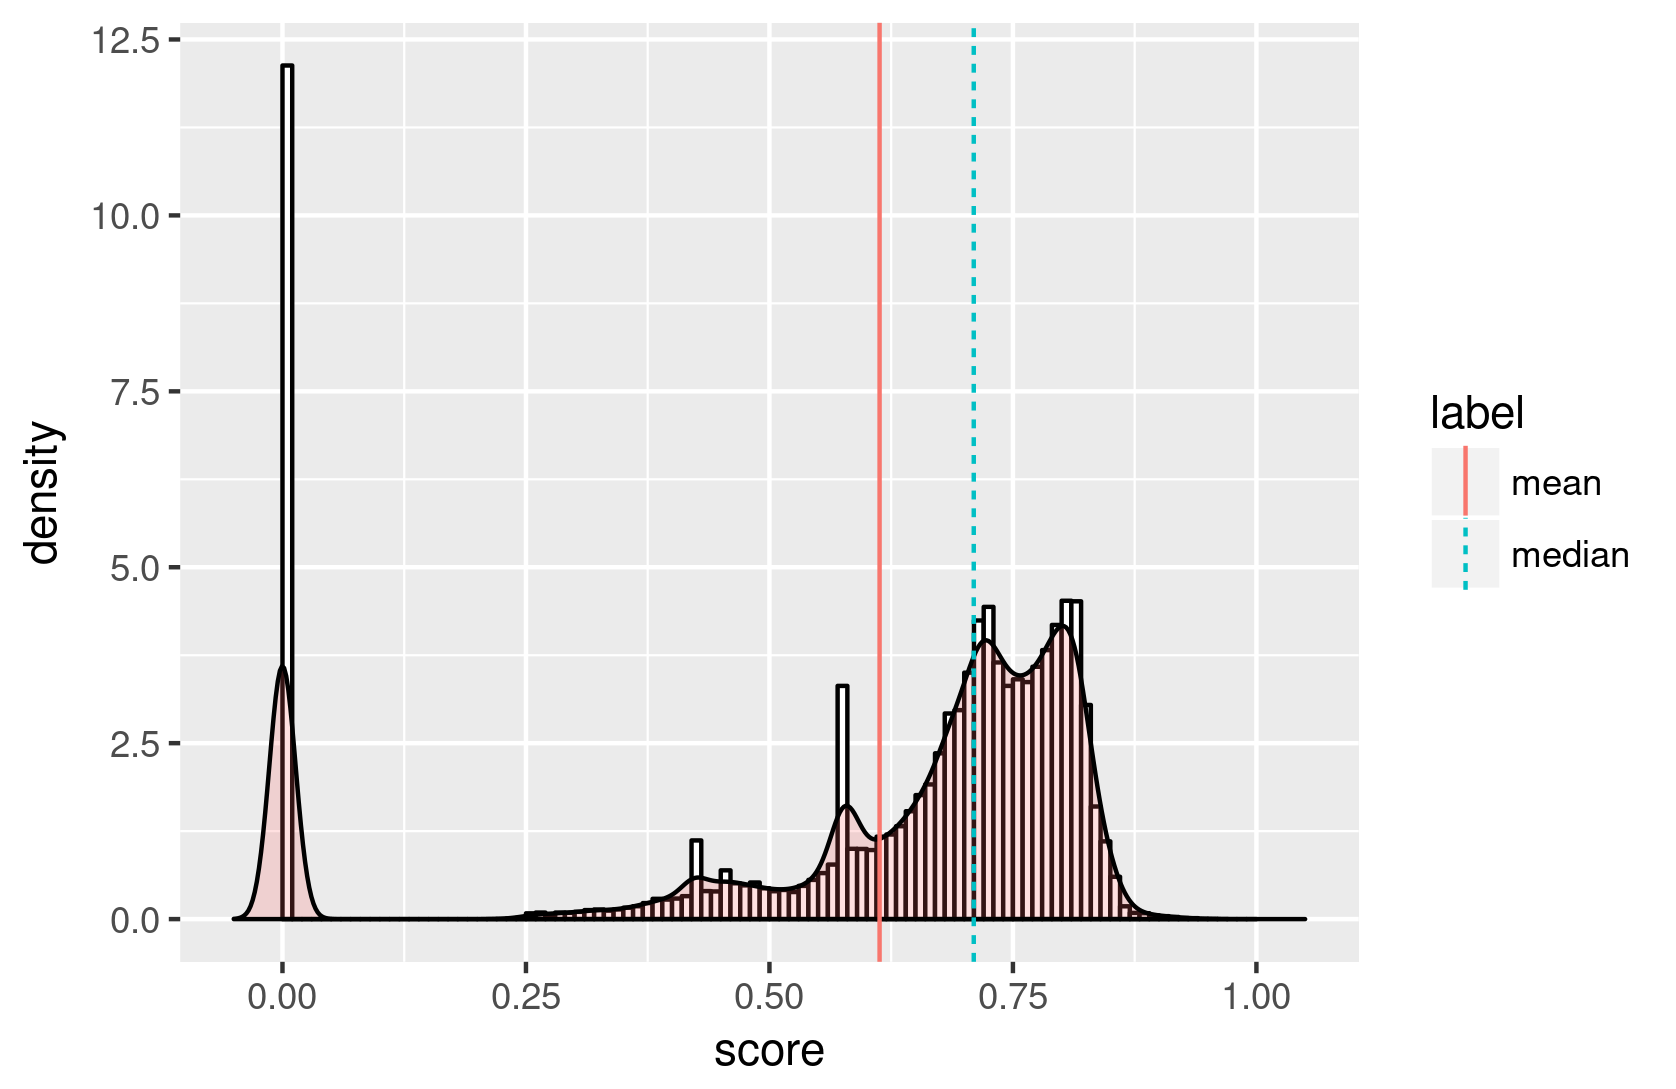
\includegraphics[width=0.8\textwidth]{figures/sa-population}
    \caption[Sample population of L-systems generated using the SA-optimized grammar distribution]{Sample population of \glspl{L-system} generated using the \gls{SA}-optimized grammar distribution}
    \label{fig:sa-population}
\end{figure}

Figure~\ref{fig:uniform-population} shows the uniform grammar distribution' sample distribution, where practically the whole population has a score of 0.
When removing all zero-scored individuals, another distribution presents itself in Figure~\ref{fig:uniform-population-no0}.
Here, a somewhat double bell-shaped distribution around the score 0.5 with a high concentration at around 0.4 is revealed for the remaining 121 individuals (0.12\% of the total).
Figure~\ref{fig:sa-population} shows the \gls{SA} grammar distribution's distribution of fineness scores.
87.87\% of the \gls{SA} sample population have a score larger than 0, compared to 0.121\% in the uniform sample population.
%Thus the \gls{SA} grammar distribution helps avoid most of the worst \glspl{L-system}.
%As the distribution is skewed to the left, the median may be a better estimate of the population average.

\begin{figure}
    \centering
    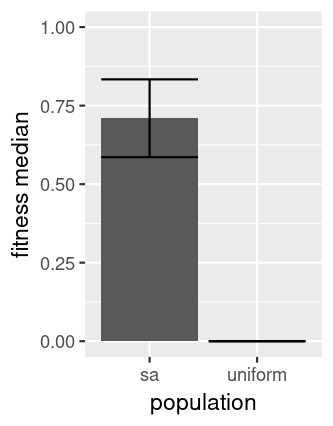
\includegraphics[width=0.4\textwidth]{figures/sa-uniform}
    \caption[Random population with uniform grammar distribution compared to SA-optimized grammar distribution]{Random population with uniform grammar distribution compared to \gls{SA}-optimized grammar distribution}
    \label{fig:sa-uniform}
\end{figure}

Figure~\ref{fig:sa-uniform} shows a comparison of \gls{L-system} populations generated by the grammar distribution found by \gls{SA} in Figure~\ref{fig:sa-progress} and a uniform grammar distribution.
The \gls{SA} grammar distribution has a median of 0.71 (MAD: 0.12), compared to 0.00 (MAD: 0.00) for the uniform grammar distribution.
A Mann–Whitney U test on the full sample suggests that the true location shift is not zero (p < 0.05, U = 608550000).
Even with all individuals with score 0 removed, the \gls{SA} grammar distribution's median score is higher with a median of 0.72 (MAD: 0.10) compared to 0.47 (MAD: 0.08), though the difference of 0.25 is smaller.
A Mann–Whitney U test on the sample without zero scores still suggests that the true location shift is not zero (p < 0.05, U = 1318100).

% might split these into separate figures and put them inbetween the above paragraphs
\begin{figure}
    \centering
    \begin{subfigure}{0.48\textwidth}
        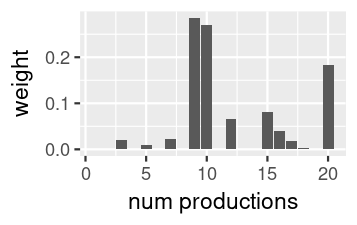
\includegraphics[width=\textwidth]{figures/sa-dist-prod}
        \caption{1*20production}
        \label{fig:sa-dist-prod}
    \end{subfigure}
    ~
    \begin{subfigure}{0.48\textwidth}
        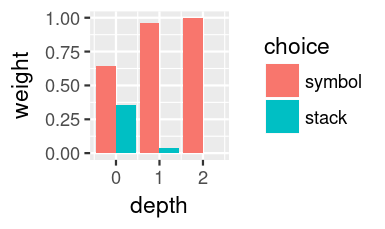
\includegraphics[width=\textwidth]{figures/sa-dist-stack}
        \caption{symbol / stack}
        \label{fig:sa-dist-stack}
    \end{subfigure}
    \\
    \begin{subfigure}{0.98\textwidth}
        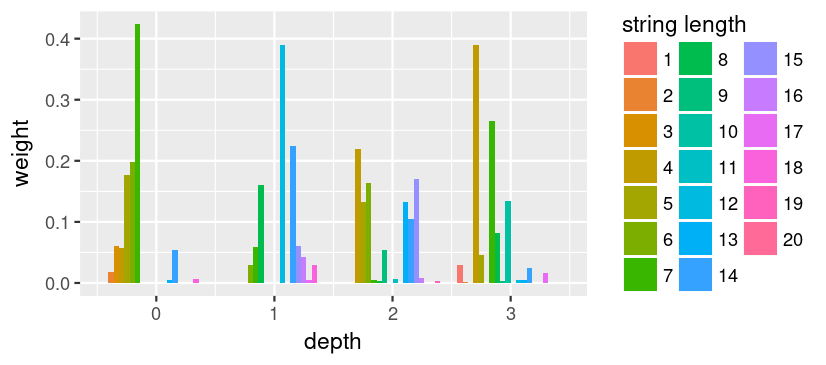
\includegraphics[width=\textwidth]{figures/sa-dist-strlen}
        \caption{1*20(symbol / stack)}
        \label{fig:sa-dist-strlen}
    \end{subfigure}
    \\
    \begin{subfigure}{0.4\textwidth}
        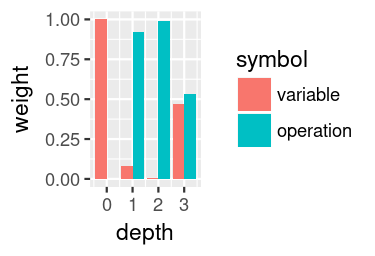
\includegraphics[width=\textwidth]{figures/sa-dist-sym}
        \caption{variable / operation}
        \label{fig:sa-dist-sym}
    \end{subfigure}
    ~
    \begin{subfigure}{0.57\textwidth}
        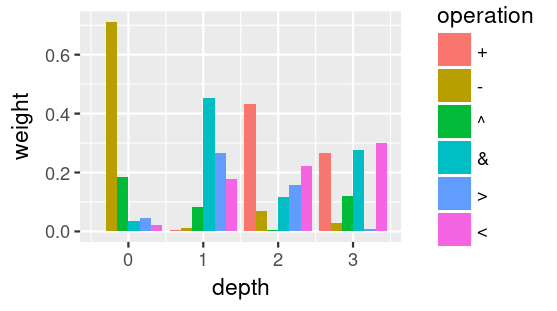
\includegraphics[width=\textwidth]{figures/sa-dist-op}
        \caption{"+" / "-" / "\textasciicircum" / "\&" / ">" / "<"}
        \label{fig:sa-dist-op}
    \end{subfigure}
\end{figure}
\begin{figure}
    \ContinuedFloat
    \begin{subfigure}{0.98\textwidth}
        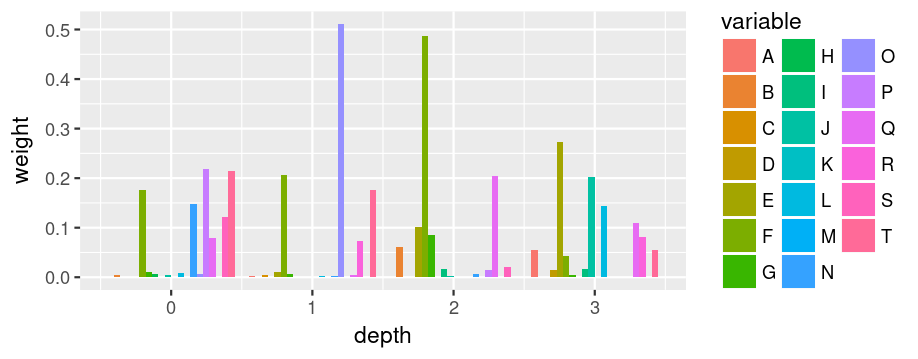
\includegraphics[width=\textwidth]{figures/sa-dist-var}
        \caption{\%x41-55}
        \label{fig:sa-dist-var}
    \end{subfigure}
    \caption[SA-optimized grammar distribution]{\gls{SA}-optimized grammar distribution. Captions are the respective parts of Listing~\ref{lst:grammar}.}
    \label{fig:sa-dist}
\end{figure}

The grammar distribution found in the SA process is shown in Figure~\ref{fig:sa-dist}.
As seen in Figure~\ref{fig:sa-dist-prod}, this grammar distribution favors around 10 production rules in the \gls{L-system}, though 20 productions is also a strong contender.
Figure~\ref{fig:sa-dist-stack} shows that it always favors symbols over stacks, starting at around 60\% symbols in the top depth, then around 90\% symbols in the next depth, and 100\% symbols in the final depth.
This makes all of the distributions at depth 3 irrelevant as they will never be used.
It favors shorter strings in depth 0, but not too short strings, as seen in Figure~\ref{fig:sa-dist-strlen}.
While in depth 1 and 2 it favors medium short and medium long strings.

Figure~\ref{fig:sa-dist-sym} shows that it only allows variables in depth 0, while its nearly the inverse in depth 1 and 2.
This is interesting as an operation has no effect if it is not followed by a variable.
Thus depth 2, along with depth 3, is not contributing anything to the plant, but depth 2 is still wasting instructions.
Depth 1 also has only about 10\% chance of a variable, meaning that most of the drawing will happen in depth 0, which in turn means less branching.

The operation distribution in Figure~\ref{fig:sa-dist-op} has a strong tendency of yawing to the right (\texttt{-}) than the left (\texttt{+}) in depth 0.
In depth 1 it barely allows yawing at all, while in depth 2 it is the opposite with a strong focus on \texttt{+}.
The other rotations (pitch and roll) also have one-sided tendencies, but not as strong.
Among all of the 20 variables available, \texttt{F} is the only variable that is an instruction, the draw line instruction.
Figure~\ref{fig:sa-dist-var} shows that it is included and is in fact one of the stronger variables in the distribution.
Only 3--4 of the variables have a strong weight in each of the depths.

\begin{figure}
    \centering
    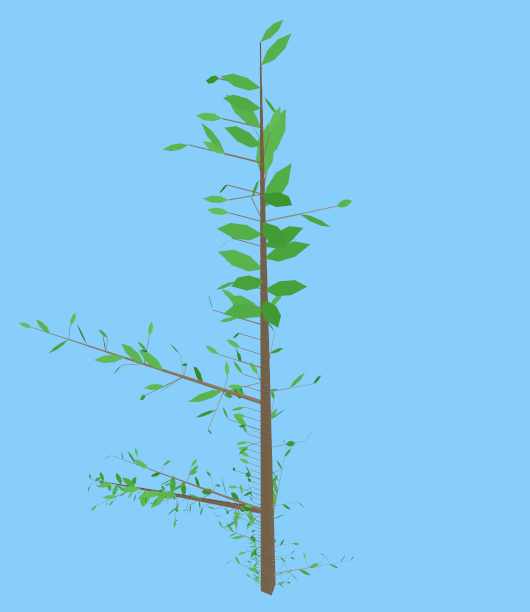
\includegraphics[width=0.6\textwidth]{figures/sa-plant}
    \caption[Example plant generated by the SA-optimized grammar distribution]{Example plant generated by the \gls{SA}-optimized grammar distribution, fitness 0.78}
    \label{fig:sa-plant}
\end{figure}

\begin{lstlisting}[caption=L-system representation of plant in Figure~\ref{fig:sa-plant}, label=lst:sa-plant, float]
axiom: NT[>>&&&&>&&&F[++++<<]]P[<<&^[>-+<+>]&><&&&&&O]P
F -> Q[O&^&&&^&<>O[<<+++++^>++<++&][++++-]&>]NT[^>R>&>[<<&<+&+&<+&+-<]<<>&&]P
L -> [O&<<>&^&&&&>]S[^<[+++-<<>>++<<+<-]^>&<<&>&&>F^>]T[<<&><^&&O&<>]
N -> N[><&<^&<<&&^&&T][&>[+-<<>+++&+&<+][+++++&><++><<^-]&&&>]PN[&&>&>T&&&&^&><<&]
P -> [&&&O>&>&&>>&&F]F[<&&&&&&>&&&&]TF
S -> [><&<&&>&]TSQS[&T<<<>[>++-+]<<&&>]T
T -> PT[>&^>&&&>&&R&&<>>]
\end{lstlisting}

% Try to connect this to the above even more.
An example of a plant generated with the \gls{SA}-optimized distribution can be seen in Figure~\ref{fig:sa-plant}, and its \gls{L-system} is found in in Listing~\ref{lst:sa-plant}.
This plant is very tall and straight, has few branches and few fractal patterns.
The \gls{L-system} goes to depth 2, but depth 2 never includes any symbols, and is therefore not relevant for the 3D model.
Depth 1 is mostly producing operators, but also an occasional variable.
There is recursion in the segment drawing as \texttt{F} produces \texttt{P} and \texttt{T} which in turn produce \texttt{F}.
Additionally, part of the recursion is inside a stack, thus allowing for fractal patterns.

\section{Evaluation of Evaluation Module}
\subsection{Method}
\textbf{RQ2} asks ``how aesthetically pleasing plants can be generated''.
\gls{DGEL} was the developed solution to this question, but to know if it can actually generate aesthetically pleasing plants or not, the evaluation module has to be analyzed and compared to how humans rank the plants.
If the ranking made by the humans agree with the ranking made by the fitness component in the evaluation module, it would suggest that the generator knows how to distinguish good plants from bad plants, and can apply its evolutionary algorithms to generate aesthetically pleasing plants.
So the hypothesis (\textbf{H4}) is: Humans agree with the ranking made by the \gls{DGEL} fitness component.
If the humans do not completely agree with the \gls{DGEL} ranking, the next question is why this is the case and what can be done to improve the rank correlation?

While the first question can be answered by quantitative methods, the second question requires support from a qualitative analysis to understand what factors are important to distinguish good generated plants from bad.
Thus an embedded design mixed-method with qualitative data as a supplementary is used~\cite{PracticalResearch}.

% Write about AHP?
A pairwise comparison of a set of \gls{DGEL}-generated plants is performed by human participants and the \gls{AHP} is used to create a ranking of all of the plants~\cite{2008Saaty}.
By using \gls{AHP}, we do not only get a ranking of the plants, but also distances between the ranks.
This is useful because humans may consider some of the plants equally pleasing, or some plants much more pleasing than others.
Finally, all of the rankings are aggregated and compared to the ranking made by \gls{DGEL} using Kendall's Tau~\cite{1938Kendall}, and dRank~\cite{2009Carterette}.
Because the human rankings only has priority weights and not absolute scores, the DGEL fitness scores are translated into weights by dividing each score by the sum of the scores such that they sum to 1.
The data fit the requirements of Kendall's Tau~\cite{2010Webber}: they are unweighted, conjoint and have a definite range.
Therefore Kendall's Tau is used to test the ranking correlation.
It also gives an indication of how correlated they are in range $[-1, 1]$, where 1 is perfectly positively correlated, 0 is not correlated and -1 is perfectly negatively correlated.
But there are two problems with this: it does not consider the relative distances between the ranks~\cite{2010Webber}, and the different participant's rankings have to be aggregated beforehand, meaning Kendall's Tau does not consider the variance between the different human rankings.
Therefore, dRank is used as an additional statistic, as it considers the distances between ranks and that there are multiple rankings aggregated together~\cite{2010Webber,2009Carterette}.
Whenever a dRank statistic is shown, the B is the bootstrap sampling size used for estimating the p-value~\cite{2009Carterette}.

As many plants as possible is desired, but humans have limited patience and the number of comparisons to rate is $\frac{n * (n - 1)}{2}$, where $n$ is the number of plants.
Therefore a limited set of plants has to be used.
The final number of plants used is based on the estimated time used on a comparison and the estimated time a participant is patient.
The plants should also be spread over the whole range of the fitness score, so that the rank comparison will be valid for the complete range.
They should also always be \textit{something} (have at least one branch), otherwise there is nothing to rate.
The ideal score range would be $[0, 1]$, but it was found difficult to generate plants with perfect 0 (with the plant being \textit{something}) and 1 scores.
Thus \gls{GE} is used to generate the worst possible plant with score above 0, and the best possible plant.
Then, $n - 2$ additional plants are generated uniformly between these two extremes.

To estimate the number of plants to rank, and to assess the quality of the survey, a three-step process is used.
First, a rough estimate is made based on researchers intuition and an assumed patience of 10 minutes.
Then, in the second step the researcher performs the pairwise comparison while measuring the time used.
Based on this and the bias of the researcher, a new estimate is created.
The third and final step is to run two or more pilot runs on another person with the previous estimates.
The time used is measured, their actions are observed and they are asked some questions at the end.
They were asked to complete the survey as described in its introduction, think aloud, tell us when they get tired and answer some questions at the end.
% Exactly which questions? Necessary?
Based on this, the number of plants is re-estimated with a margin in case of bias, a new set of plants is generated, quality issues are fixed, and the pilot is run once more to confirm the new estimate.

Participants were sampled using convenience sampling and snowball sampling.
As such, the results may not be generalizable to the whole population, but they may be used as an indication as to what is important in an aesthetically pleasing plant.
Convenience sampling was selected because of time and resource restrictions, and snowball sampling was added as a means to gather further samples.
Participants were found by asking friends, family and acquaintances either by direct conversation or by posting publicly on social networks including Facebook, Google+ and Twitter.
The participants were asked to share the survey to others, and a sharing link was shown at the end of the survey, thus allowing for a snowballing effect.
Before the survey link was shared with others, four people were observed directly while taking the survey, with a method similar to that of the pilot runs.
This both allowed for deeper qualitative data and final adjustments to the survey.

\subsection{Survey Design}
\label{sec:survey-design}
% link to consent?
% link to survey?
The survey consists of a consent form that they need to agree with, a pre-questionnaire, a description, the pairwise comparison, a post-questionnaire with the results, and finally a thank-you page with the sharing link.
The pre-questionnaire is intended to map the demographic and what relation they have to plants and games.
The description describes the pairwise comparison task, what they should do in it, and what to expect at the end.
The post-questionnaire is intended to find out how much the participant agrees with the ranking calculated by \gls{AHP} or why they do not agree, and what they find important in plants.
Finally, the thank-you page is used to assure the participant that they have completed the survey, give them the option to see or share their results, and share the survey to others.

In the pre-questionnaire the participants are first asked about their age, gender, education and occupation.
They are then asked ``how often do you work with plants? Including all types of interactions with plants, such as gardening, household plants, photography, etc.'', and ``how much do you like plants in general?'' on a 5-point Likert scale.
Their purpose is to see if their relation to plants affects how they rank the plants.
Finally, they are asked ``how often do you play video games?'' on a 5-point Likert scale.
This is to see if their relation to video games affects how they rank the plants.
A person that regularly works with plants or enjoys looking at plants in nature may expect something different in a plant than a person who regularly sees plants in video games.

During the description of the task, they are recommended to enter fullscreen so that they do not have distractions and so that the plants can be viewed as big as possible.
They are also asked to try a different browser or withdraw if the plant visualization is not working as expected.
This is because the quality of the visualization may affect their ratings.

\begin{figure}
    \centering
    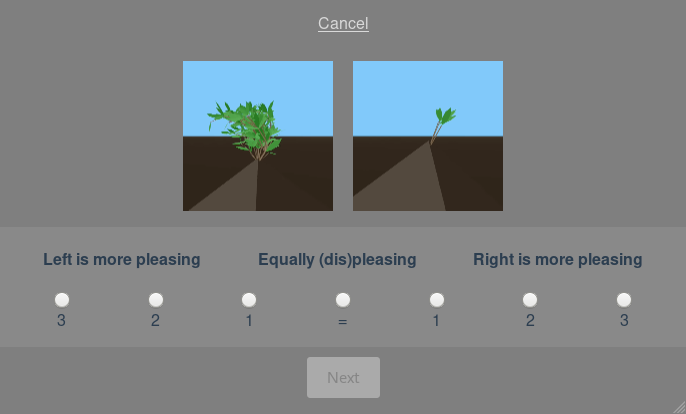
\includegraphics[width=1.0\textwidth]{figures/pairwise}
    \caption{Pairwise comparison task as viewed on a small screen}
    \label{fig:pairwise}
\end{figure}

Figure~\ref{fig:pairwise} shows the comparison task.
It is kept as simple as possible to avoid distractions, and a neutral gray background color is used to avoid the perceived hue or brightness of the plants to be shifted.
Two plants are visualized side by side as looping videos of a camera rotating around the plant so that all sides of the plant is seen.
In addition, the camera adjusts its height and distance from the plant so that all of the plant can be viewed.
The rotation happens at a balanced speed that lets the user view all of the plant in a short amount of time, while being slow enough to let them study it.
% The pilot confirmed that the speed was good.

The video runs at 60 frames per second (FPS) to give a smooth experience, to match the monitor refresh rate and to match what is commonly used in games.
They are encoded as both VP9 WebM and H.264 MPEG-4 to support a wide range of browsers.
According to Mozilla Developer Network (MDN), H.264 is supported in most browsers, but depends on platform support, and their support may be removed as the format has patents make them ``unfit for the open web platform''~\cite{mdn-video}.
Therefore the videos are encoded in both formats and VP9 is the preferred one if both are supported.

They are compressed as much as possible to reduce load times, while still keeping a near lossless visual quality as to not bias the comparisons.
Both are encoded with the FFmpeg tools\footnote{FFmpeg website: \url{http://ffmpeg.org/}}.
Both the FFmpeg Wiki and Google Developers recommend using Constant Quality for WebM~\cite{ffmpeg-vp9,google-vp9}.
They recommend CRF values from 15 to 35, and based on the resolution and Google Developers's resolution and CRF value matrix, a CRF of 32 is used~\cite{ffmpeg-vp9,google-vp9}.
For H.264, according FFMpeg Wiki a CRF value of 17--18 can be considered ``visually lossless''~\cite{ffmpeg-h264}.
Thus, 18 was selected as it allows the files to be smaller than 17.
Based on this, WebM is encoded with the parameters \texttt{-quality best -crf 32 -b:v 0}, while MPEG-4 is encoded with \texttt{-preset veryslow -crf 18}.
\texttt{-quality best} and \texttt{-preset veryslow} enable better quality per file size at the cost of slower encoding~\cite{ffmpeg-h264}, but as the videos are encoded offline, the encoding time cost is not important.

The participant is presented with three categories to choose between: left is more pleasing, they are equally (dis)pleasing, and right is more pleasing.
If they find one more pleasing they need to rate how much pleasing it is on a scale of 1 to 3.
The original \gls{AHP} method uses an 8-point scale for each side~\cite{2008Saaty}, but this is too detailed for a ``normal human'', % cite or argue
and so it was reduced to 3 points which allows for a low, medium and high rating.
Based on feedback from the pilot run, the ``equally (dis)pleasing'' option was labeled ``='' instead of ``0'' because ``0'' seemed like it meant that the plants were bad.
``(dis)'' was also added based on the feedback because without it it seemed like it meant that the plants were good.
With these changes, the participant should be less reluctant to select ``equal''.

By pressing the ``next'' button, the participant is presented with new pairs until all have been rated.
The pairs are presented in random order and with random placement (left or right), as to not make the order create a bias.

\begin{figure}
    \centering
    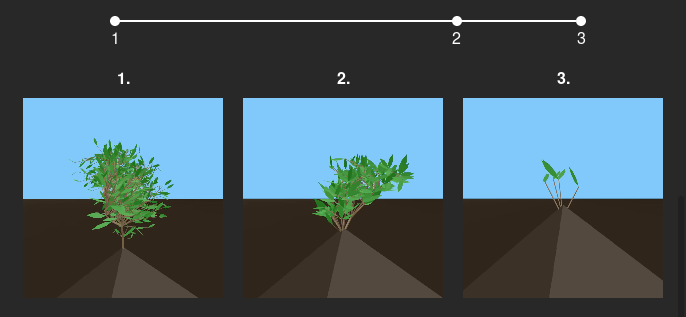
\includegraphics[width=1.0\textwidth]{figures/rank}
    \caption{Example rank resulting from human rating of plant pairs}
    \label{fig:rank}
\end{figure}

The post-questionnaire asks some questions and displays the resulting order of the plants.
Figure~\ref{fig:rank} shows an example of the resulting order.
The dots on the white line represents the relative distance between the plants, and the plants themselves are shown in order below.
% Explain how this is done.
In this example, the plant ranked as the best has a larger distance to the second than the second has to the third.
The participants are asked if they ``agree with the ranking of the plants shown below'', and if they do not ``strongly agree'', they are asked ``why do you not strongly agree with the ranking?''
This can help determine if the method of ranking the plants with \gls{AHP} is valid.
Next they are asked the most important question: ``What would you say separates good plants from bad plants in the ranking?''
This is useful to be able to do a qualitative analysis of why the human ranking does not match the fitness ranking, if they do not match.
Finally, they are asked for ``other comments'' in case they have something useful to add that do not fit the other questions.

The final thank-you page contains a congratulation, a link to revisit their results, and a link to share the survey.
This share link contains a token that indicates who it was shared from.
With this data the snowball effect can be tracked.
Though, there is nothing preventing them from sharing the original link, thus losing this information.

\subsection{Implementation}
No web-based application that matches the design of the survey was found.
Thus a single-page web-application was created~\cite{CodePairwise}.
It uses the Vue.js JavaScript framework in the front end\footnote{Vue: \url{https://vuejs.org/}}, the Rocket web framework for Rust in the back end\footnote{Rocket: \url{https://rocket.rs/}}, and MongoDB to store the data\footnote{MongoDB: \url{https://www.mongodb.com/}}.
Multiple other libraries were used both in the front end and back end, but the aforementioned are the most central.
As the application is a on-off application, only meant to be used for the survey, and fairly simple, the choices of technology and architecture were based on experience, convenience and preferences.
Most of the technology used had recently been used in another project by the researcher, and thus allowed for code re-use and rapid development.

The application uses a client--server architecture, as shown in Figure~\ref{fig:pairwise-architecture}, where the server consists of two layers: API and DB.
The client uses a Vue Component for each page described in the Survey Design, and URL routing is handled by Vue Router.
The Components communicated directly to the API layer using a custom REST API, to for example register a participant or get the pairs of plants to evaluate.

The API layer is written in Rust and uses the Rocket framework to implement the API.
Multiple routes are defined based on the requirements of the client.
It communicates directly to the MongoDB database using the \textit{mongodb} Rust library.

When a participant registers, they receive a private token that is kept in the URL in the client throughout the whole survey.
This token access to submit and retrieve their data.
They also receive a public token that represents the participant, but does not grant access to their data.
Thus, this public token is used in the share link to identify who shared it.

The participant participates only in a specific \textit{task}.
A task is a set of plants that are to be evaluated, and the system may contain multiple tasks.
While only one task is used during the survey, allowing multiple tasks lets the researcher experiment with the application without affecting the real data while developing or during the survey.

The database contains three collections: \textit{user}, \textit{sample} and \textit{weight}.
\textit{user} stores all data relating to the user and is uniquely identified by the private and public tokens individually.
\textit{sample} stores data about one of the plants, such as its name and the task it is part of.
Finally, \textit{weight} stores the rating submitted by one user for one pair of plants and is uniquely identified by the user and the two plants together.

Finally there is a command-line interface (CLI) available to extract the data either as raw data or as calculated priority weights using \gls{AHP}.
Because of this, a separate module \textit{stats} in the API layer contains the common functionality used by both the API and the CLI.

\subsection{Results}
\subsubsection{Plants}
The lowest possible plant fitness score found by \gls{GE} was 0.27, and the highest was 0.97.
Thus, the plant fitness scores used are: 0.27, 0.34, 0.40, 0.46, 0.53, 0.59, 0.65, 0.72, 0.78, 0.84, 0.91 and 0.97.
The plants will be referred to with their fitness score.
All of the plants can be viewed in Figure~\ref{fig:survey-plants} in Appendix~\ref{app:survey-plants}.

\subsubsection{Participants}

There were 56 people that registered.
Of those, 37 completed ranking the plants.
This means that 34\% of the 56 participants did not rank the plant, of which many likely are people that unintentionally registered multiple times.
Those who did not complete the ranking of the plants are excluded from the analysis.
Finally, one of the 37 did not submit the post questionnaire.

The demographic of the participants is mainly 20--30 year old (65\%) males (78\%) with a bachelor or higher degree (76\%) in information and communication technologies (49\%).
The age ranges from 21 to 69.
Science \& engineering and service \& sales were also strongly represented with 16\% and 14\% respectively.

\begin{figure}
    \centering
    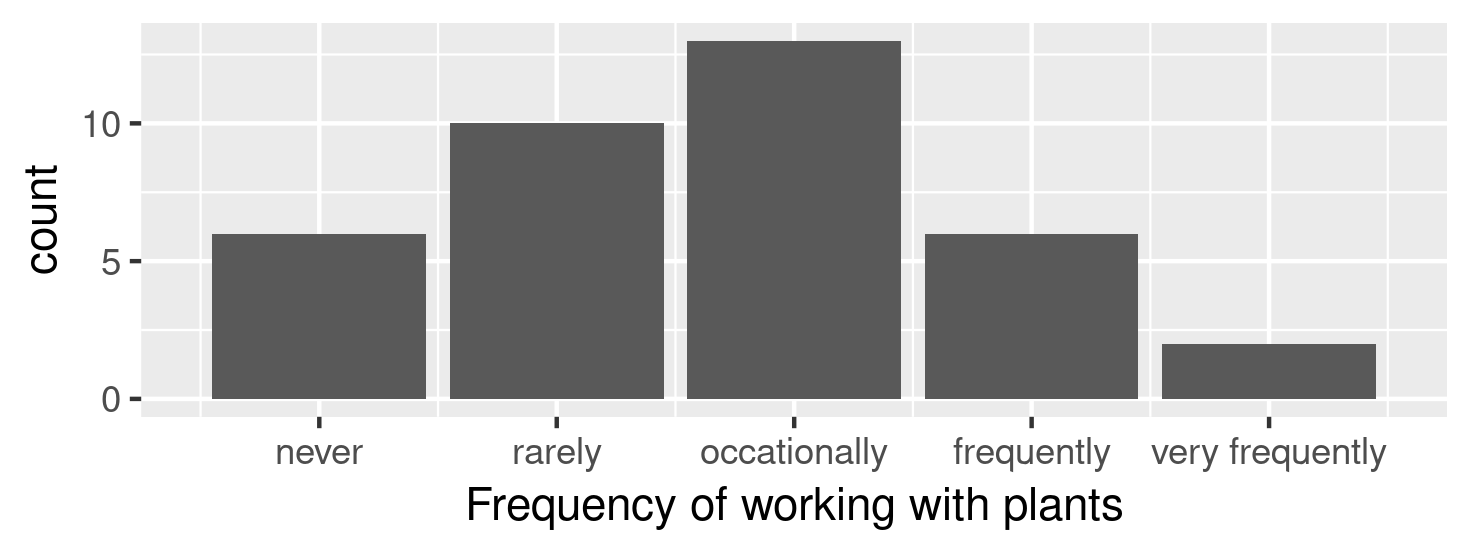
\includegraphics[width=0.8\textwidth]{figures/user_plant_work}
    \caption{Participants' frequency of working with plants}
    \label{fig:plant_work}
\end{figure}

\begin{figure}
    \centering
    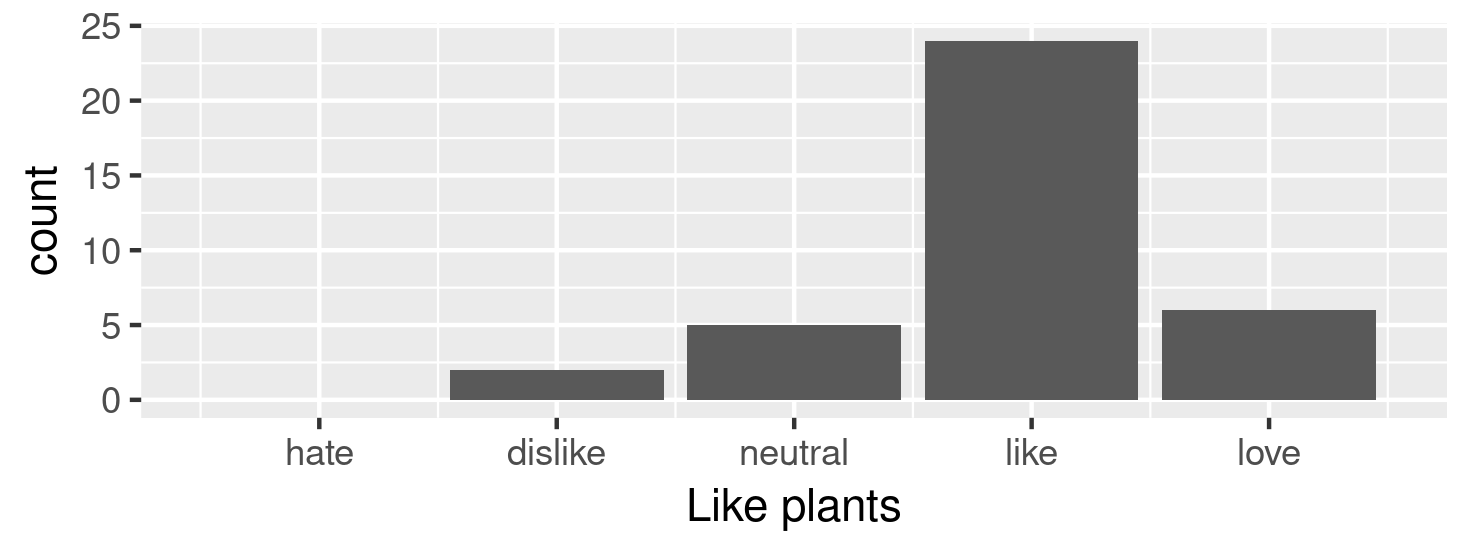
\includegraphics[width=0.8\textwidth]{figures/user_plant_like}
    \caption{How much participants like plants}
    \label{fig:plant_like}
\end{figure}

\begin{figure}
    \centering
    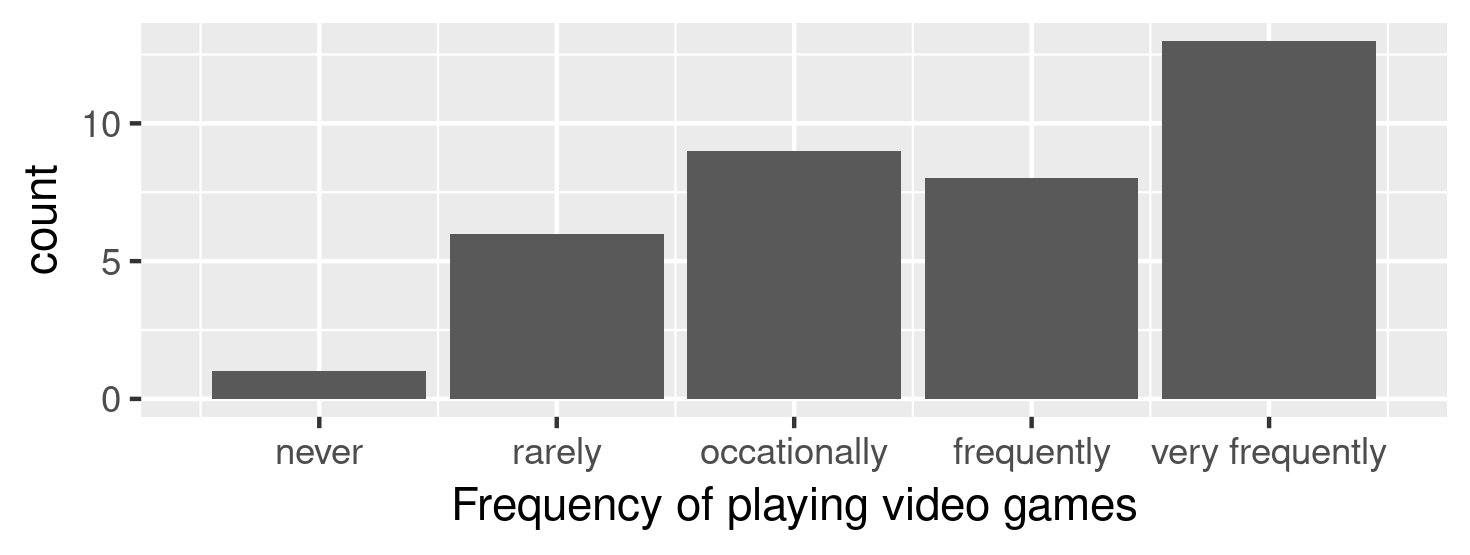
\includegraphics[width=0.8\textwidth]{figures/user_games}
    \caption{Participants' frequency of playing video games}
    \label{fig:games}
\end{figure}

As seen in Figure~\ref{fig:plant_work}, the participants tend to occasionally work with plants with a skew towards less frequently.
Figure~\ref{fig:plant_like} shows that while the participants usually do not work much with plants, they tend to like them (64.87\% like them and 16.22\% love them), no one hates them, and only 5.41\% dislike them.
Thus the participants generally have a good relationship with plants.
Finally, in Figure~\ref{fig:games} there is a tendency towards playing video games frequently (median = frequently, 56.76\% play at least frequently), and only 2.7\% never play games.

There was only 1 participant that received the share link from another participant.
Still, only around 25 people were directly asked to participate, and only 15 confirmed that they participated.
Additionally, it is not expected that all of the people contacted directly did participate.
Thus, at least 12 participants, and likely more, must have received the link from another person.

\subsubsection{Ranking Agreement}
\begin{figure}
    \centering
    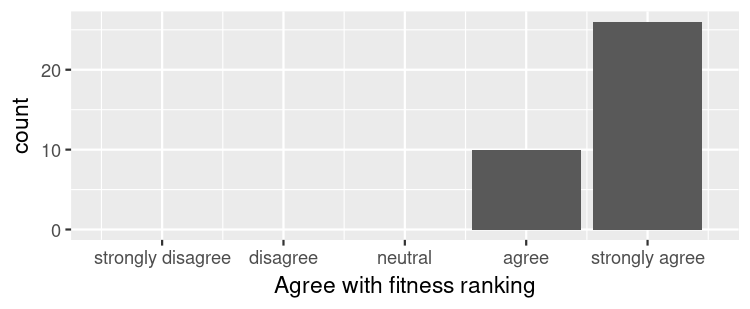
\includegraphics[width=0.8\textwidth]{figures/agree}
    \caption{Human agreement with the AHP ranking}
    \label{fig:agree}
\end{figure}

As seen in Figure~\ref{fig:agree}, the participants always agree with the ranking made by \gls{AHP}.
73\% strongly agree, while the rest agree.
The ones that did not strongly agree have to explain why.
These explanations were categorized into four categories based on the content: null, invalid, position and distance, as shown in Table~\ref{tab:agree-why}.
While the participants were obligated to write a reason, one participant was able to not write anything and is therefore categorized as \textit{null}.
Some explanations contained comments that were not answering the question, which could be because of misunderstanding the question, misinterpretation of the scale, or laziness.
For example, the comment ``I never agree strongly with online tests'', indicates that they use the scale differently, and actually completely agree with the ranking.
Therefore, these comments were categorized as ``invalid''.
Finally, two categories were actual reasons to why they did not strongly agree: \textit{position} and \textit{distance}.
A plant being positioned in a wrong rank was the most common reason, as it was commented by 5 of the participants.
In all cases they only wanted to move one plant.
Only one commented on the distance between the ranks.

\begin{table}
    \centering
    \begin{tabularx}{\textwidth}{| l | X | l |}
    \hline
    \textbf{Category} & \textbf{Description} & \textbf{Occurrences} \\ \hline
    null & No comment & 1 \\
    \hline
    invalid & The participant did not answer the question, but commented something irrelevant & 3 \\
    \hline
    position & Feels that a plant is in the wrong position and wants to change its rank & 5 \\
    \hline
    distance & Feels that the distances between some ranks are either too short or too long & 1 \\
    \hline
    \end{tabularx}
    \caption{Reasons as to why 10 of the participants did not strongly agree with AHP ranking}
    \label{tab:agree-why}
\end{table}

\subsubsection{Correlation Between Human and Fitness Ranking}
\begin{figure}
    \centering
    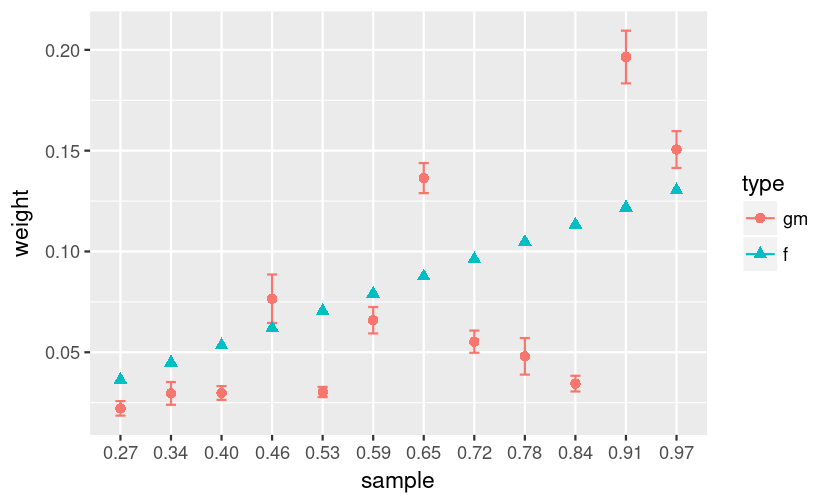
\includegraphics[width=1.0\textwidth]{figures/weights}
    \caption[Fitness score plus geometric mean and arithmetic mean of priority weights]{Normalized fitness score (f) plus geometric mean (gm) of human priority weights, with standard error}
    \label{fig:weights}
\end{figure}

The fitness ranking and the human aggregated ranking are shown together in Figure~\ref{fig:weights}.
From this it can be observed that both agree on the three worst and the two best rankings, while in-between these there are big differences.
For example, 0.65, 0.72, 0.78 and 0.84 are ordered in the reverse order, and are far from the fitness ranking.
0.53 and 0.84 is also ranked as bad as the three worst by the humans, while the fitness ranks them higher.
Finally, humans prefer 0.91 much more over 0.97, which is reverse of the fitness.
Still they do somewhat agree with the ranking of 0.49 and 0.59, while they are reversed.

dRank calculates a ranking distance of 16.67 (p = 0, B = 10000), meaning that the human rankings are significantly different from the fitness ranking, and we reject the hypothesis that they are the same.
Still, this does not mean that there is no positive correlation between the rankings, only that they are not equal.
Kendall's tau is 0.55 (p < 0.05), indicating a positive correlation, though only at about 55\%.

With the two best ranks (0.97 and 0.91) and three worst ranks (0.27, 0.34, 0.40) removed, thus looking only at the ``middle'' part, the dRank distance is 5.21, (p = 0, B = 10000), and Kendall's tau is -0.33 (p >= 0.05), indicating no correlation in either direction (\textit{middle} in Table~\ref{tab:rankstats}).

\subsubsection{Analysis of Bad Correlation}
\begin{figure}
    \centering
    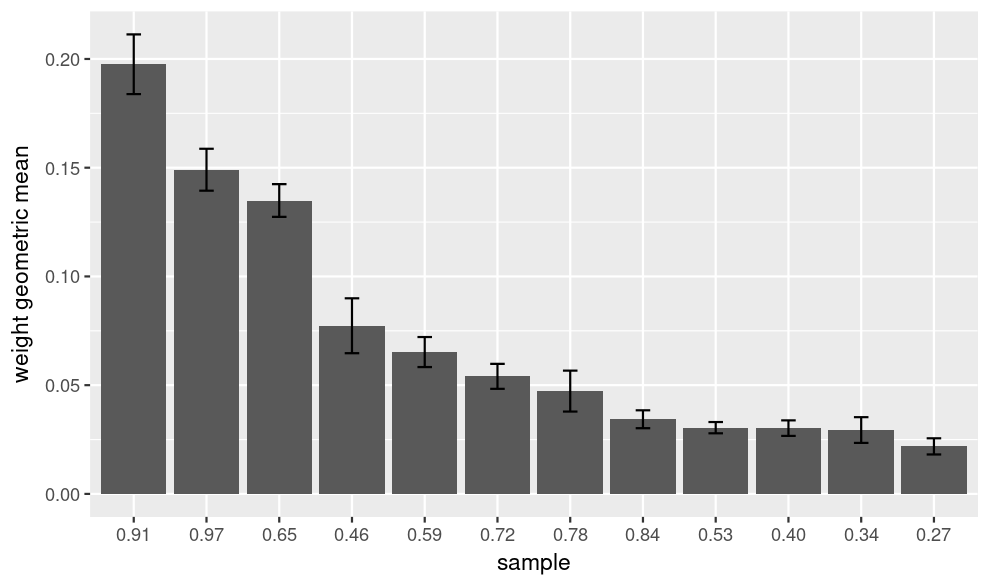
\includegraphics[width=1.0\textwidth]{figures/weights_bar}
    \caption[Priority weights from human plant ranking]{Priority weights from human plant ranking, with standard error}
    \label{fig:weights-bar}
\end{figure}

Figure~\ref{fig:weights-bar} shows the ordered human ranking.
Both agree that 0.27 is the worst plant.
0.34, 0.40, 0.53 and 0.84 seems to be ranked as equally bad, just above 0.27.
0.78, 0.72, 0.59 and 0.49 seem to be slightly climbing in score.
0.91 is clearly in first place, while 0.97 and 0.65 are possibly on a shared second place.
The standard errors are smaller on the bad plants than on the good plants.
Both 0.84 and 0.46 were moved 5 ranks down and up respectively, almost swapping places.
0.84 is the worst, having a difference in weight between its neighbor of 0.12 compared to 0.05 for the 0.46 plant.

\begin{figure}
    \centering
    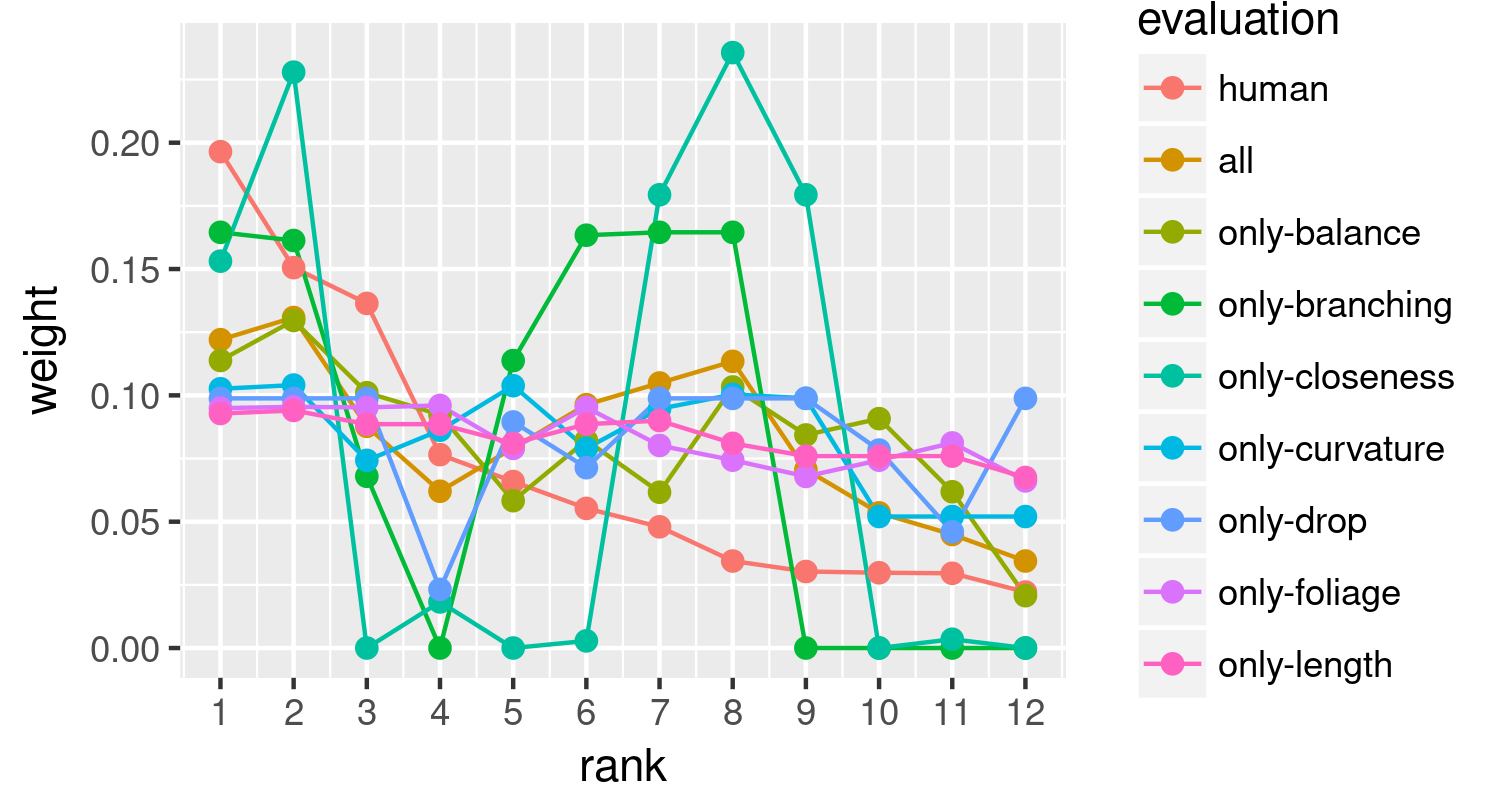
\includegraphics[width=1.0\textwidth]{figures/fitcmp-only}
    \caption[Human ranking compared to fitness ranking and its components]{Human ranking compared to fitness ranking (\textit{all}) and its components. The ranking on the x-axis is the human ranking.}
    \label{fig:fitcmp-only}
\end{figure}

\begin{table}
    \centering
    \begin{tabular}{| l | l | l |}
    \hline
    \textbf{Ranking} & \textbf{Kendall's Tau} & \textbf{dRank} \\
    \hline
                all & 0.55 (p = 0.01)  & 16.67 (p = 0, B = 10000) \\
             middle & -0.33 (p = 0.88) & 5.21 (p = 0, B = 10000) \\
        only-length & 0.75 (p = 0.00)  & 20.99 (p = 0, B = 100) \\
       only-foliage & 0.57 (p = 0.01)  & 17.01 (p = 0, B = 100) \\
       only-balance & 0.49 (p = 0.02)  & 16.67 (p = 0, B = 100) \\
     only-curvature & 0.45 (p = 0.02)  & 16.63 (p = 0, B = 100) \\
     only-branching & 0.36 (p = 0.07)  & 25.43 (p = 0, B = 100) \\
     only-closeness & 0.14 (p = 0.27)  & 16.63 (p = 0, B = 100) \\
          only-drop & 0.13 (p = 0.30)  & 21.67 (p = 0, B = 100) \\
            removal & 0.79 (p = 0.00)  & 16.67 (p = 0, B = 100) \\
     removal-middle & 0.52 (p = 0.07)  & 5.21 (p = 0, B = 100) \\
    \hline
    \end{tabular}
    \caption{Rank correlations between various versions of the fitness and the human ranking}
    \label{tab:rankstats}
\end{table}

% Should be in discussion?
Figure~\ref{fig:fitcmp-only} compares the human ranking against fitness ranking and each individual fitness metric.
The fitness ranking has a clear problem of scoring the ranks 5--9 too high, which creates a ``bump'' in the curve.
Two metrics that stand out --- closeness and branching --- look like may be a major cause of this bump, as they themselves have an even larger bump.
Additionally, the drop metric seems to be in a disagreement with the human ranking.
These observations are also supported by Kendall's Tau and to some degree dRank, as seen in Table~\ref{tab:rankstats}.
Kendall's Tau indicates that all three metrics are not correlated (p >= 0.05).
Branching also has a low correlation compared to the other metrics, but relatively higher than the other two.
dRank supports that drop and branching have a low correlation, but disagrees with Kendall's Tau on the closeness ranking.

\begin{figure}
    \centering
    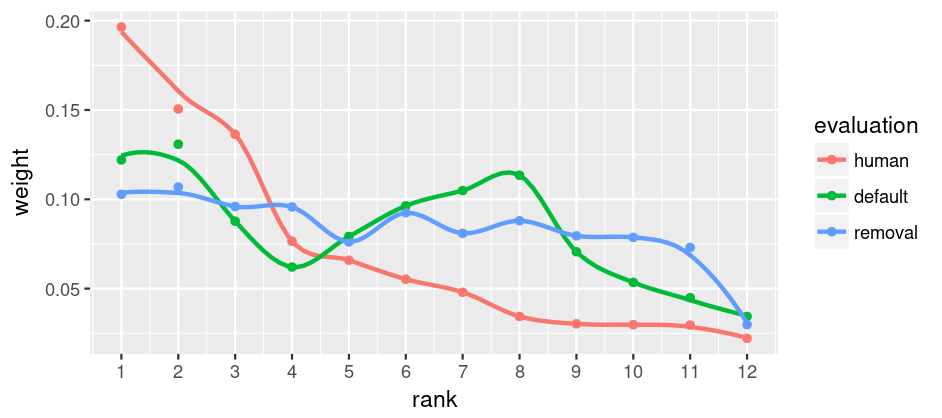
\includegraphics[width=1.0\textwidth]{figures/fitcmp-removal}
    \caption[Human ranking compared to fitness ranking (all) and a version with branching, drop and closeness metrics removed (removal)]{Human ranking compared to fitness ranking (all) and a version with branching, drop and closeness metrics removed (removal). The ranking on the x-axis is the human ranking.}
    \label{fig:fitcmp-removal}
\end{figure}

These findings together suggest that these three metrics may have a bad effect on the correlation of the human and fitness rankings.
This is supported by the plot of the \textit{removal} evaluation in Figure~\ref{fig:fitcmp-removal} and its rank correlation in Table~\ref{tab:rankstats} (\textit{removal}).
The ``bump'' has been removed, but there are instead some ``waves'' in the center part that disrupts the ranking.
Additionally, there is less distance between the two best plants and the third best plant, and a larger distance between the worst and second worst plants.
The Kendall's Tau is 0.79 (p < 0.05), which is an improvement of 0.24, while dRank indicates no difference.
Additionally, the correlation in the middle region has also improved as seen by \textit{removal-middle} in Table~\ref{tab:rankstats}, though Kendall's tau is still not statistically significantly different from 0 (p >= 0.05).

\subsubsection{Human Perception of Aesthetically Pleasing Plants}
All participants were asked openly what they would say ``separates good plants from bad plants in the ranking''.
These comments were categorized into factors and the number of participants who mentioned them was counted.
The factors were split into two: directional factors and directionless factors.
Directional factors have a clear understanding of what is better and what is worse, while directionless factors only understand what is important without knowing which direction is better or worse.
They can be found in Table~\ref{tab:factors-dir} and Table~\ref{tab:factors-nodir} respectively.

\begin{table}
    \centering
    \begin{tabularx}{\textwidth}{| l | X | l |}
    \hline
    \textbf{Category} & \textbf{Description} & \textbf{Occurrences} \\
    \hline
    natural & Looking ``natural'' is positive & 8 \\
    \hline
    artificial & Looking ``artificial'' is positive & 1 \\
    \hline
    healthy & Looking ``healthy'' is positive & 2 \\
    \hline
    details & Higher level of detail is positive & 4 \\
    \hline
    environment & Environmental effects on plants is positive & 3 \\
    \hline
    chaos & Chaos is negative & 5 \\
    \hline
    symmetry & Symmetry is positive & 1 \\
    \hline
    asymmetry & Symmetry is negative & 1 \\
    \hline
    patterns & Recognizable patterns is positive & 1 \\
    \hline
    more leaves & More leaves is positive & 5 \\
    \hline
    balanced leaves & Balanced amount of leaves is positive & 2 \\
    \hline
    lush & Higher leaf density is positive & 2 \\
    \hline
    leaf pitch & Leaves pointing up is positive & 1 \\
    \hline
    even spread & Branches and leaves spread out evenly is positive & 3 \\
    \hline
    small & Small plant size is negative & 3 \\
    \hline
    curves & More and soft curves is positive & 3 \\
    \hline
    upwards & Growing upwards is positive & 3 \\
    \hline
    sideways & Growing sideways is positive & 1 \\
    \hline
    complexity & Complex branches is positive & 2 \\
    \hline
    clipping & Branches or leaves growing inside the ground is negative & 2 \\
    \hline
    obstructions & Obstructions is positive & 1 \\
    \hline
    straight & When plants have few leaves they look better if they grow straight up & 1 \\
    \hline
    dynamic & Simple plants are better when dynamic & 1 \\
    \hline
    arrangement & Simple plants are better when well arranged & 1 \\
    \hline
    visible branches & Dense amounts of visible branches is negative & 1 \\
    \hline
    balanced & Center of mass close to trunk is positive & 1 \\
    \hline
    uniform bend & A uniform bend of the branches is positive & 1 \\
    \hline
    \end{tabularx}
    \caption{Directional factors}
    \label{tab:factors-dir}
\end{table}

\begin{table}
    \centering
    \begin{tabular}{| l | l |}
    \hline
    \textbf{Category} & \textbf{Occurrences} \\
    \hline
    leaf amount & 3 \\
    leaf distribution & 2 \\
    leaf density & 1 \\
    leaf size & 1 \\
    form & 3 \\
    symmetry & 1 \\
    growth & 1 \\
    branch amount & 1 \\
    branch placement & 1 \\
    character & 1 \\
    \hline
    \end{tabular}
    \caption{Directionless factors}
    \label{tab:factors-nodir}
\end{table}

The abstract category ``natural'' was mentioned the most (8 times).
Many participants said that plants looking ``natural'' looked better, sometimes contrasted to ``artificial'' plants.
The word ``natural'' was often used as a dependent factor of other independent factors.
For example a comment said ``[...]the stems seemed to be perfect (angles), hence not natural'', which implies that ``natural'' is an important factor and the angles of the stems is a factor that affects the ``natural'' factor.
There was only one participant who suggested the opposite, i.e. that artificial-looking plants looked good, or more specifically ``interesting [...] as I do not expect to see a lot of symmetry in plants''.

``more leaves'' was the second most occurring category (5 comments).
Comments that fit into this category either suggest that the plants with more leaves look better, or that plants with less leaves look worse.
There were also comments that said that a balanced amount of leaves is positive (2 comments).

The third most occurring category is ``detail'', which says that a higher level of detail in the plants is a positive factor.
Simple or small plants were often commented as having too little detail and thus not looking natural.
There are three categories that are specifically for these types of plants: straight, dynamic and arrangement.
They suggest that simple plants look better when growing straight upwards, being more dynamic or well arranged.

\begin{table}
    \centering
    \begin{tabularx}{\textwidth}{| X | X | X | X |}
    \hline
    Abstract & Structure & Foliage & Other \\
    \hline
    natural, artificial, healthy, character, chaos, dynamic, growth, arrangement &
    symmetry, asymmetry, patterns, even spread, form, small, curves, upwards, sideways, complexity, visible branches, balanced, uniform bend, branch amount, straight, branch placement &
    more leaves, balanced leaves, lush, leaf pitch, leaf amount, leaf distribution, leaf density, leaf size &
    clipping, obstructions, details, environment \\
    \hline
    \end{tabularx}
    \caption{Grouping of factors}
    \label{tab:factor-groups}
\end{table}

The factors were grouped into four groups: abstract, structure, foliage and other.
The abstract group contains factors that are not quantifiable and thus more abstract in nature.
For example it is not straight forward to quantify how ``natural'' a plant looks.
Structure contains factors that consider the structure of the plant, i.e. the features of the branches and their patterns.
Foliage contains factors that consider the leaves on the plant and their individual properties or the foliage as a whole.
Other are factors that do not fit in the other groups.
The grouping of the factors is shown in Table~\ref{tab:factor-groups}.

% Turning off specific metrics mostly results in little change.
% Turning off branching improves the first valley and a little bit the bump, though it skews the bump to the right.
% Analyzing 0.53 and 0.84 indicates that the curvature may be rewarding plants that do not look curvy.
% Analyzing 0.46 it looks very lush, which may not be rewarded enough.
% Branching uses mean, but should use median.
% Curvature uses mean, but should use median.
% Length should be more cosine-like.
% Curvature should assume that the longest branch, not the ``straightest'', is the straight edge.
% Shorter segments and improved leaf heuristic could help with level of detail on small plants.
% Organic = natural

% "clean" interpreted as not chaotic.
% "foliage coverage" interpreted as "leaf distribution"
%
% Plant ranked 8 (0.84)
% - Looks artificial.
% - Few leaves
% - Not lush
% - Low level of detail?
% - Not growing upwards
% - Not complete
% - Center far from trunk
% - Metric says supurb curvature, but this is not visible
%
% Plant ranked 4 (0.46)
% - lush+
% - chaotic-

% !TEX root = ../Masters.tex
\chapter{Discussion}
\section{Grammatical Evolution}
\label{sec:discuss-ge}
As evident from the results, the \gls{DGEL} \gls{GE} process performs significantly better than the brute-force approach, and the statistically significant difference in their scores support that \gls{DGEL} \gls{GE} finds plants with better fitness scores than brute-force does (\textbf{H1}).
Additionally, the fact that \gls{GE} was five times faster than brute-force means that even if both methods produce just as good individuals, \gls{GE} will be faster at doing so.

The difference in duration is an interesting case because both \gls{GE} and brute-force generate the same amount of individuals, and while brute-force only fills a vector of random numbers, \gls{GE} must do both a crossover and mutation which are more complex functions.
It is likely that this is caused by the tournament sampling and the fact that \gls{GE} improves the population with each generation, reducing the complexity of the L-systems, thus reducing the time spent evaluating them.
For each individual that should be in the population of the next generation, tournament selection picks a pair of individuals (with a tournament size of 2) randomly from the current population, evaluates them and allows the best one to become part of the next generation.
Because of this, tournament sampling may pick the same individuals multiple times, which means the cached evaluation is used, and some individuals may not be picked at all.
The fitness evaluation of a chromosome is expensive because it has to generate the L-system, interpret it into a 3D structure and then run each metric on this structure, so this may have a big impact.
% The chance that an individual in the population is, in the case of a population size of 800,
% TODO: What is the average percentage of evaluated individuals? Does this correlate with the difference in duration?

\section{Simulated Annealing}
The clustering of the movements around the current score in the \gls{SA} process (Figure~\ref{fig:sa-progress-close}) indicates that the mutation function used has a good locality, i.e. that the neighboring grammar distributions are fairly close in terms of score.
At the same time, the somewhat uniform spread of scores between the current score and 0 indicates that there are some mutations that have bad locality.
Additionally the clustering at exactly zero indicates that there are some mutations with the worst possible locality.
These bad locality mutations could be caused by some parameters in the grammar distribution having a cascading effect.
For example if the \texttt{symbol / stack} distribution in depth 0 suddenly changes from 0.5/0.5 to 1.0/0.0, all depths below will be excluded and thus most of the parameters in the distribution will be irrelevant.
The clustering at exactly 0 is more likely to be caused by the fitness measure, because it has a limit on the amount of \gls{L-system} instructions and when that limit is reached the plant is in all cases scored 0.
It could also happen if the distribution does not allow for any \texttt{F} symbols as without it no branches will be drawn in the 3D model.
%, indicating a discontinuity in the fitness metric.

Because brute-force with the \gls{SA}-optimized distribution has a higher percentage of non-zero fitness scores than with a uniform distribution, one of the benefits of using an optimized distribution is that it avoids many of the problematic ``nothing'' plants that are scored 0.
This is good because even though the non-zero scores in majorly zero-scored grammar distributions may have good scores (as evident from Figure~\ref{fig:uniform-population-no0}), a large amount of zero-scored plants will lead to a slow search process.

Because of the large amounts of zero-scored plants, as evident from Figure~\ref{fig:sa-population} and~\ref{fig:uniform-population}, the median should be a better measure for central tendency.
Based on this, it may be argued that the median should be used instead of the mean when measuring the grammar distributions as well.
But since a large amount of zero-scored plants is bad, which is something the grammar distribution should consider, the mean could be argued as being a better measurement for the grammar distribution.
Additionally, by using the median, it will suddenly jump from a good score to zero if the amount of zero-scored plants goes below 50\%.
Thus comparing distributions that are at around this limit by the median may be unfair, so the mean is more appropriate.

Based on the observation that the \gls{SA}-optimized distribution restricts itself to three depths, setting a hard limit of maximum four depths may not have been too limiting.
At the same time, other \gls{SA}-optimized distributions may want to allow four depths, and there may be a point above four depths where very good plants are found.

Comparing the \gls{SA}-optimized grammar distribution in Figure~\ref{fig:sa-dist} with the generated 3D model in Figure~\ref{fig:sa-plant}, similarities can be drawn, thus indicating that the grammar distribution has an effect on the resulting plants.
For example, the fact that depth 1 only has variables, and deeper depths barely has any variables, is reflected in the tall and straight tree with few branches.
It is impossible for the generator to produce \glspl{L-system} with operators in depth 0, and thus only straight lines are possible in that depth.
While there is a possibility of drawing angled lines through the lower depths, because of the low rate of variables in them, it is less likely.
The only reason that there are branches coming out of the trunk is of the string ``\texttt{[\&\&\&O>\&>\&\&>{}>\&\&F]}'' in rule \texttt{P}.
This string pitches down and rolls before drawing a line so that the branch will actually stick out from the trunk rather than grow inside it.
% WHY NOT MEDIUM STRING LENGTHS? WHY A VALLEY BETWEEN THESE?
% random? impossible to say without more tests...

The strong weight of \texttt{F} in the grammar distribution indicates that the \gls{SA} process understood the importance of \texttt{F}.
Without the \texttt{F} variable, the \glspl{L-system} would have no branches and thus get score 0.
Additionally the fact that only a small amount of the other variables are strongly weighted could be explained by the fact that a large amount of variables decreases the likeliness of the same variable appearing multiple times and therefore not being useful (e.g. only in successors).

With a significant difference in the medians by a large amount, it is clear that ``an \gls{SA}-optimized grammar distribution can find better individuals than a uniform grammar distribution'' (\textbf{H2})
The additional fact that the \gls{SA}-optimized grammar distribution produced a significantly smaller proportion of zero-scored individuals further supports this hypothesis.

As there was no statistically significant difference between \gls{GE} with a uniform grammar distribution and random brute-force with an \gls{SA}-optimized grammar distribution, hypothesis \textbf{H3} that random brute-force with an \gls{SA}-optimized distribution can perform as well as \gls{GE} with a uniform grammar distribution is supported.
This is rather interesting, because this indicates that only pre-optimizing the grammar distribution can have a significant beneficial impact on the search, at least as strong impact as \gls{GE} has.
Though it should be kept in mind that, as discussed in Section~\ref{sec:discuss-ge}, \gls{GE} uses significantly shorter time to perform the search than a random brute-force search on the same amount of individuals, which may mean that even if random brute-force with an \gls{SA}-optimized distribution can perform as well as \gls{GE} with a uniform grammar distribution, the latter may be faster.

The statistically significant difference in the medians of \gls{GE} with an \gls{SA}-optimized distribution and \gls{GE} with a uniform distribution supports hypothesis \textbf{H4} that ``GE with an SA-optimized grammar distribution can find better individuals than with a uniform grammar distribution''.
This indicates that a grammar distribution optimized by \gls{SA} not only can improve random brute-force search, but can also improve \gls{GE}, and possible other \glspl{EA}, to perform better with stricter parameters, thus decreasing its duration.

%GE with an \gls{SA}-optimized grammar distribution can find better individuals than with a uniform grammar distribution (H3)

\section{Fitness}
% results?
Excluding participants that had null or invalid reasons, only 16\% of the participants (6 people) did not strongly agree with the \gls{AHP} ranking, and all of those still agreed with the ranking.
Thus, there is a strong support that the \gls{AHP} pairwise comparison ranking method is valid.
Still there are issues with it according to the participants.
5 (83\%) of them think that the rank of one plant is wrong, while 1 (17\%) thinks that the distances between some ranks are wrong.
This could either be an effect of the participants not being experts in the field or indicate an issue with doing pairwise comparison where they do not see the whole picture.

The designed or adapted metrics used in the fitness function were clearly not perfect measures for how aesthetically pleasing plants are.
Still, as both humans and the fitness function both agreed on the two best plants and three worst plants, the metric may have the baseline of how to measure the ``pleasingness'' of plants.
It is only in the middle region where the fitness metrics get confused and disagrees with the humans.
With Kendall's tau indicating no correlation in the middle region, it is a strong indication that this region has the biggest potential for improvement.
Interestingly, dRank indicates that the distance between the rankings the middle region (5.21) is smaller than the complete ranks (16.67). % I don't know how to interpret this...
This effect could be caused by the reduction of the number of systems (plants), which the dRank distance is highly dependent on~\cite{2009Carterette}.
In any case, the p-value of dRank is still 0, indicating that they are still not correlated.
Based on this, the hypothesis that humans agree with the ranking made by the \gls{DGEL} fitness component (\textbf{H5}) is rejected, and the next question should be why they do not agree and what could be done to improve the agreement.

The categorization of factors that humans find important can give an overview of what the fitness function should include or exclude.
Directional factors are directly useful since they can be used to change a fitness metric's direction or create new metrics for the fitness function.
Directionless factors are less useful on their own, but they indicate the importance of the factor, and thus can either be used to adjust the weight of a metric or a directional factor.
For example, ``leaf amount'' is a directionless factor that can be used to strengthen the directional factors ``more leaves'' and ``balanced leaves''.
Both types of factors can be used to analyze why the current metrics do not correlate with the human ranking.

With the standard errors being smaller on the bad plants than on the good plants, it might indicate that it is more likely that humans agree on what looks bad compared to what looks good.
% The below not actually mentioned in the results...
This is also supported by the observations of the four first participants where they often spent more time comparing good plants to each other, and said themselves that this was difficult.
% Thus maybe plants above a certain threshold should be used?

Drop, closeness and branching were found as the metrics that had the worst correlations, and the correlation statistic on the rankings with these metrics removed supports this.
It is clear that these metrics either incorrectly measure pleasingness or measure something else.

Closeness is most likely not a good metric for how aesthetically pleasing a plant is, because its purpose is to prevent a the physically impossible phenomenon of branches clipping into each other, something that the human in most cases does not notice.
It could in fact have a negative effect on the fitness function, because one of its artifacts is that multiple leaves will appear on the same branch segment when multiple branches clip into each other.
This artifact was indicated by one participant in the survey as ``creating an interesting symmetry'' that they liked.
A possible solution could be to remove this metric and use a heuristic or physical simulation to make the branches collide with each other and thus bend away from each other.
Other metrics, such as \textit{branching}, could then reward or punish the branching point like in other cases.
The artifact of multiple leaves at the same segment could be added as a heuristic, or it would be allowed with an \gls{L-system} grammar such as the one in Listing~\ref{lst:grammar2}.

The drop metric is a similar type of metric in that it also aims to prevent physically impossible situations.
It was originally designed to prevent plants from growing down through the ground, but as the plants viewed in the survey were placed on a pyramid-shaped hill, this was not an issue.
Thus the reason it had a bad correlation is most likely similar to that of the closeness metric.
This could also be solved with a heuristic or physical simulation, like with the other metric.

The branching metric is a more interesting case as it is more aimed at measuring the realism of the plant, but still has a bad effect on the overall fitness function.
From the plot in Figure~\ref{fig:fitcmp-only}, it seems to work well in distinguishing the good from the bad plants, but it creates a bump in the middle region from rank 5 to 8.
Looking at the specific plants in this region, there could be multiple reasons for this bump.
The plant at rank 5, when counting the branches coming out from the bases, looks like it has an OK amount of branches, but is generally simplistic and small, which are negative factors that could be overshadowing the other factors such as the branching.
The next plant has a balanced amount of branches, but that value may have been overshadowed by its simplicity, leaf scarcity and symmetry which are all mostly negative factors as indicated by the humans.
The plant at rank 7, when looking at it, has a large amount of branches coming out of a single point, indicating that either the metric is not correctly measuring the branching or the branches are clipping into each other, thus allowing more branches to appear from the same point.
The latter is a likely cause because the closeness metric is punishing it with the maximum possible value (-1.0), meaning that there is at least one point where branches completely overlap.
%It is likely that it triggers negatively on factors such as chaos, visible branches and even spread, that could overshadow other factors.
The last plant visually has slightly too many branches, which is also supported by the \textit{branching} metric (0.38, where the best is 1 and worst is -1), but is not on the negative side.
The humans also rated this plant the highest of all four middle plants.
Compared to the plants ranked above it, it looks smaller, simpler and less lush, which may again overshadow the branching.

Based on the above analysis of the middle plants, it could be argued that the size, complexity and lush factors should be included in the fitness or more heavily weighted.
None of them are directly included in the current fitness metric, but \textit{length}, \textit{branching} and \textit{foliage} should cover parts of them.
Additional metrics could include something that measures the spread of the plant in addition to its length (size factor), density of branches (complexity) and density of leaves (lush).
They should prefer bigger, denser and more lush plants, but they should also have a balance where at some point it becomes too much.
Additionally, because three of these plants were relatively small, and humans indicated that when this is the case their level of detail is too low, metrics measuring the size and complexity factors could dynamically be weighted more based on their score, overshadowing the other metrics if necessary.

\section{Research Questions}
As parametric S2L-systems are the most flexible \gls{L-system} variations, one can argue that they should be the best choice for \gls{L-system} plant models that ``are appropriate to represent plants both found in nature and not found in nature'' (\textbf{RQ1}).
While these \glspl{L-system} were not used in this research and other literature because of their complexity, based on the results, simple D0L-systems, specifically represented by the grammar in Listing~\ref{lst:grammar}, seem to be able to model both natural and artificial plants.
This is because, based on the comments from the participants, both ``natural'' and ``artificial'' was found as important factors either describing bad or good plants, thus indicating that the generated plants was able to look both natural and artificial.
An important factor to consider is that the \gls{L-system} grammar only enabled branches, and adds branch widths and leaves as simple heuristics.
Thus, these results are only applicable if these heuristics or \gls{L-system} grammar that replace these heuristics are used.
While D0L-systems may be appropriate to represent both natural and artificial plants, it may not be the best.
More flexible models, such as IL-systems, parametric \glspl{L-system}, stochastic \glspl{L-system}, or their combination as parametric S2L-systems may be better as they allow for more detail.

That the \gls{GE} performance improved with increasing crossover rates indicates that the crossover operation has a positive effect on the evolution.
This could suggest that the \gls{DGEL} chromosome representation could be a good choice for ``[combining different \glspl{L-system}] into new plants'' (\textbf{RQ1}).
It does not directly indicate that one single crossover will retain or improve the fitness of the plant, but using it in a \gls{GE} process either targeting a good fitness or the same fitness as the parents could work.
For example, the initial population could consist of 50\% of each parent, the mutation rate could be set to 0.1 and crossover rate to 0.5.
These recombination rates focuses more on crossover than mutation, thus being more likely to keep some of the features in the chromosome, but are still able to reach a fitness of 0.92.
Alternatively, since the \gls{DGEL} generation process is able to produce fit individuals, it could be used together with a fitness measure of how similar the offspring is to its parents.

While the fitness function used does not correctly measure how aesthetically pleasing an \gls{L-system} plant is, based on the analysis, it has the potential for it.
Because the rankings done by humans only indicate the relative differences between plants and not how pleasing a plant is on an absolute scale, it is difficult to say if \gls{DGEL} manages to generate aesthetically pleasing \gls{L-system} plants (\textbf{RQ2}).
What we can say is that \gls{DGEL} is able to generate both plants that are less aesthetically pleasing and more aesthetically pleasing.

To know if the ``more aesthetically pleasing'' plants are actually aesthetically pleasing, they would have to be evaluated in a different manner.
For example, the plants from this survey could be used in another survey where participants are asked if they find the presented plants aesthetically pleasing or not.
This could also indicate a threshold in the fitness function which must be reached for a plant to be pleasing.
This assumes that the fitness function and humans agree on the ranking.

% Where is the data for this? need to ditch it if I can't add results for it.
Looking at the observations of participants in the survey, some said that certain plants looked realistic or natural.
Based on this and the assumption that realistic or natural plants are aesthetically pleasing, this could suggest that \gls{DGEL} is able to generate aesthetically pleasing \gls{L-system} plants (\textbf{RQ2}), though this is a stretch.
% generalize?

With the in-depth analysis of one \gls{SA}-optimized grammar distribution, there is an indication that the \gls{DGEL} grammar distribution together with \gls{SA} can focus the parameter space onto certain areas that contain plants with particular properties.
It shows that the grammar distribution can restrict the stack dept, adjust in which depth the drawing instruction should appear and control which rotations should be more prominent.
Thus, by using multiple grammar distributions, multiple ``generators'' that each generate somewhat unique plants could be used together to create a larger variations of plants.

Additionally, the 37 different factors of aesthetic plants found from the qualitative data from participants, indicate that just the 12 different plants generated have different properties and can therefore be varied.
For example, both natural, artificial, chaos, symmetry, asymmetry, curves, straight, sideways, environment and details were found as factors.
They are all different or opposites of others, and since the participants were asked specifically about the plants that they ranked, this shows that there was a clear variation in those 12 plants.
The fact that these 12 plants were randomly generated by \gls{DGEL} suggests that this may apply generally for \gls{DGEL} and that another 12 new plants may also be varied.
Thus, using \glspl{L-system} with \gls{GE}, and optionally using grammar distributions with parameter optimizers is a method of generating varied \gls{L-system} plants (\textbf{RQ3}).
Some hand-picked plants that were generated with \gls{DGEL} can be found in Appendix~\ref{app:plants}.

All of this together suggests that the \gls{DGEL} architecture and algorithm is a viable solution to generating \gls{L-system} plants ``that are aesthetically pleasing, varied and could be used to create offspring similar to its parents'' (\textbf{RQ0}).
With the additional support of hypotheses \textbf{H2}, \textbf{H3} and \textbf{H4}, \gls{DGEL} (with help from \gls{SA}) is shown to be more efficient than plain \gls{GE}, and the fact that an \gls{SA}-optimized grammar distribution to a high degree helps to avoid zero-scored plants, indicates that it, and thus \gls{DGEL} as a whole, better handles complex parameter spaces.
% It can ``generate plants'', they are ``aesthetically pleasing'', they are ``varied'', and their model could potentially ``be used to create offspring similar to its parents''.

\section{Implications of Findings}
The concept of \gls{DGEL} is not restricted to \glspl{L-system}.
By removing the L in \gls{DGEL}, thus becoming Distribution-based Grammatical Evolution (DGE), the same methods may be applicable to other grammar-based systems.
Particularly the novel approach of using a grammar distribution for \gls{GE} is a method that other problems may benefit from.

Clearly, based on the tests of an \gls{SA}-optimized distribution's performance (\textbf{H2}, \textbf{H3} and \textbf{H4}), using a grammar distribution is a significant benefit.
Particularly interesting is to see the optimized grammar distribution applied to random brute-force perform as well as \gls{GE}, and possibly even better if there was more leeway in the score (there was no room for improvement).
Combined with the indication that the grammar distribution improves the performance of \gls{GE}, it shows that a grammar distribution can be a significantly useful tool in the evolutionary computing toolbox.

First of all this means that \glspl{L-system} can be generated more efficiently, and more complex L-systems can be generated, resulting into more, better and varied 3D plants, something \gls{PCG} and thus the game industry and consumers can benefit of.
% Additonally, since \glspl{L-system} can be used to model other game content, such as missions, spaces and levels~\cite{PCG_5}, the same benefits may also apply to other content than plants.
Secondly, \gls{DGEL} applied to other grammar-based problems can be just as useful.
While only the generation of \glspl{L-system} was studied, the results (except for the aesthetics) will most likely be reflected in other grammar-based problems.
This means that a complete series of grammar-based problems can also benefit from using optimized grammar distributions.
Again this is something \gls{PCG}, and thus the game industry and consumers, can benefit of because grammars can be used to generate other game content such as missions, spaces and levels~\cite{PCG_5}.
Another good example of its benefit is in the use of grammars to generate and evolve computer programs~\cite{1998Ryan}.

In more general or abstract terms, the grammar distribution is a probability distribution.
Therefore our findings suggest that accompanying an \gls{EA} with a probability distribution, and optimizing it using optimization techniques, can improve its efficiency in complex spaces, allowing for faster searches and more varied solutions.

% Not always useful, e.g. when you can't pre-optimize a distribution or don't have computation power to do it live, or need to equally explore all aspects of the space.

% It can help focus the solutions on particular aspects that may be more useful for a set of problems.
% A simple example is to for example use a distribution that focuses on the multiplier operator when doing \gls{GP} to solve a problem.
% It could also be used to discover properties of good solutions, like how the \gls{SA}-distribution clearly focused on the \texttt{F} variable, which could lead to new insight and understanding.

\section{Limitations}
There are limitations to the findings, especially regarding the variations in plants and the fitness evaluation.
Only one \gls{SA}-optimized grammar distribution was studied, and only one plant generated with that grammar distribution.
While this gave an in-depth view on this part of \gls{DGEL}, the external validity of the results is questionable.
It is possible that \gls{SA} finds similar grammar distributions each time and thus does increase the variation of the plants.
The variation within and between different grammar distributions (including both optimized and uniform) should be studied to see if this is generally true or not.

There is a big limitation in the sampling method used and the sample of humans found for the evaluation of the fitness metric.
As seen from the overview of the demographics, the sample is highly biased and thus does most likely not represent the population.

Another limitation is that the \gls{GE} parameters found may not be the optimal parameters.
For example, the tournament size did not have an effect on the performance of the \gls{GE} process, which may be caused by the large population size and number of generations already being good enough.
It might be the case that a larger tournament size may lead to better performance with smaller population size and fewer generations.
In fact, tournament has an increasing selection intensity with increasing tournament size~\cite{1995Blickle}, meaning that the fitness should change faster with larger tournament sizes.
The same problem may apply to the other parameters as well.
This limitation does not affect the rest of the results, it only means that the \gls{GE} parameters could likely be improved.

As heuristics are used for both branch widths and leaf placement, the results may not apply to \glspl{L-system} that include leaves and widths as parts of the grammar.
A grammar like that would have more dimensions and therefore be more complex to search, thus the results may be different.
The results could both be worse or better.
For example the benefit of using \gls{GE} or \gls{SA} may be even larger when the space is more complex, or the space may be too complex for them to perform well.
Especially the particular parameters used, for example the \gls{GE} parameters, may not be applicable for other \gls{L-system} grammars.
Additionally, using other \glspl{L-system}, like parametric SIL-systems introduce even more dimensions to the search space, which may have the same problem.

Finally each person only saw one plant alone, which is unusual in nature.
Realistically plants would be surrounded by other plants, either of the same species or of different species, which will likely have a significant effect on the perception of the plant.
The perception of the plant may also be different depending on the context it is in.
For example a potted plant in the window inside a house may have different criteria for being aesthetically pleasing than a plant in the garden, or a plant found in the wild.

% symbols over stacks: PROBABLY CAUSED BY THE INSTRUCTION LIMIT, WHICH IS A LIMITATION.

% % !TEX root = ../Masters.tex
\chapter{Related Work}
% IF I WANT TO KEEP THIS, I NEED TO CONNECT IT TO MY FINDINGS.
Xueqiang and Hong developed a generalized L-system method, called GLSM, that better follows botanical principles and increases the expressive ability of L-systems~\cite{2012Xueqiang}.
They emphasize the importance of a stochastic property in the L-systems to reflect botanical principles.

Wensheng and Xinyan model grass with stochastic L-systems and trees with parametric L-systems~\cite{2010Wensheng}.
For the tree models, they create one L-system where four parameters determine the branching angles and branch lengths.
They show how two different set of parameter in the same L-system can generate two different looking trees, and how adding stochastic multiples to the parameters can generate more naturally looking trees.
This is different from stochastic L-systems, because here they multiply stochastic values with parameters in the productions, while stochastic L-systems select productions stochastically.

%Niklas pioneered artificial evolution of L-systems in 1986. % Can't find copy of paper. Only have one source from another paper. Remove this?
Jacob argues that manually inferring an L-system from a real plant seen in nature is a difficult and tedious task involving several steps~\cite{1994Jacob}.
Some of these steps can be automated using evolutionary algorithms, specifically defining L-systems, comparing the generated plant with the real plant and correcting the L-system based on how it matched.
Based on this, Jacob defines three parts of evolutionary L-system inference: generation functions that create L-systems within some constraints, evaluation functions that measure the fitness of the interpreted L-system, and modification and selection functions that allow editing of L-systems with evolutionary techniques.

To evolve the L-systems, Jacob uses Genetic Programming (GP) techniques introduced by Koza~\cite{1992Koza}.
The difference is that Jacob uses higher-order building blocks for generation and modification of expressions.
A pool of expression patterns is defined that contains several expressions that each are represented in a tree structure.
Expressions can be combined using pattern matching, such that if a leaf node of an expression matches a root node of another expression, they can be combined.
Thus, an L-systems may be built by plugging together expressions in various ways, and the resulting L-system is always guaranteed to be valid.

Jacob defines multiple genetic operators, such as mutation and crossover.
Mutation replaces a subterm of an expression with another equivalent subexpression.
Crossover exchanges to subexpressions between two parents.
Both operators use pattern matching to find subexpressions in the L-system that can be modified.
Multiple patterns may be defined for each operator and are ranked such that if there is a match with multiple patterns, the one with the highest rank is selected.

The technique described by Jacob is shown to evolve a 3D L-system based on requirements that it should have a complex structure and leaves within a certain cubic boundary.
Jacob took this method further and showed that it could evolve L-systems that looked more like plants with certain requirements~\cite{1995Jacob,1996Jacob,1996Jacob-2}.

Mock continues Jacob's work, but works directly with L-system strings instead of expressions~\cite{1998Mock}.
It is thus more of a Genetic Algorithm (GA) technique rather than a GP technique.
The L-systems used are simple 2D interpreted L-systems that only have one node rewriting rule with branching.
The successor of this single rule is used as the genetic representation in the genetic algorithm.
Two genetic operators are used: crossover and mutation.
Crossover finds a random substring in each parent with equal number of branching brackets and exchanges them.
Mutation also finds a random substring the same way, but replaces it with a new randomly generated string instead.
To select individuals from the population that should be used for the next population, both humans and a fitness function have been used independently.
Humans manually assigned fitness to the phenotypes and selected one individual to keep.
When using humans, the generated L-systems started as weed-like or random doodles and ended up with simple 2D plants.
The fitness used was a simple ``tall and wide plants preferred'' function that ended up generating objects that looked less like pants than the human-selected samples.

Ashlock et al.\ use an evolutionary algorithm to evolve both the grammar and the interpreter parameters at the same time~\cite{2006Ashlock}.
This resulted in a larger variety of generated plants.
They pack the grammar and interpreter parameters as real parameters, which made it possible to solve it as a real parameter optimization problem.

Corchado et al.\ use genetic algorithms to grow plants over time, as they argue that L-systems alone inefficiently simulate growth and change over time~\cite{2009Corchado}.
They define the genotype as a compact string representation of a production rule, and the phenotype as the visualized plant.
The contact string representation consists of the predecessor and the successor connected by the ``='' character.
E.g.\ the production $F\rightarrow FF$ would be the string ``F=FF''.
Crossover is performed by selecting two strings based on their fitness and swapping two substrings between the two strings.
They mutate the string in two different ways: either by randomly changing a character in the string with another, or randomly changing a substring in the string with another.
The crossover and mutation needs to ensure that the string is still syntactically correct.
This mainly involves making sure the branching brackets always have a matching start and end bracket.
To solve this, they use Mock's solution~\cite{1998Mock}, where they only select strings with a balanced number of start and end brackets, which may also be zero brackets.

Beaumont and Stepney use Grammatical Evolution (GE) on L-systems to evolve them~\cite{2009Beaumont}.
GE is ``an evolutionary algorithm (EA) that can evolve complete programs in an arbitrary language using a variable-length binary string''~\cite{2003Oneil}.
Beaumont and Stepney do crossover by selecting random parents and selecting a random crossover point.
The crossover point is different for each parent, to allow variation in genome length in the children.
Elitism is used to allow the most fit genomes to pass to the next generation without being mutated.
They find that elitism is a significant advantage and that certain alterations to the grammar have a significant effect.

% !TEX root = ../Masters.tex
\chapter{Conclusion}

This thesis explored how to improve plant L-system generation, particularly with the goal of being usable for combining plants.
The idea behind this is to be able to create a virtual world where people may grow and cross-breed plants.
For people to enjoy this world, the plants should be aesthetically pleasing.
They should also be varied and so that the people may get new experiences.
Finally the plants should be modeled in a way such that they can be combined into new plants via cross-breeding.
Thus, the research question is formed: How can plants be generated that are aesthetically pleasing, varied and could be used to create offspring similar to its parents?

Previous research on L-system generation has been focused on restricted L-system grammars and with fitness functions that aim at generating realistic plants.
Multiple L-system versions have been used, including D0L-systems, parametric D0L-systems, and parametric DIL-systems, which have then been evolved using evolutionary algorithms including GA, GP and GE.
Both automated fitness evaluation of L-systems, human evaluation and similarity evaluation have been used as selections strategies in the evolutionary algorithms.
Several different metrics have been used to measure the fitness of a plant, mostly aiming at evaluating the survivability of the plant, though some use humans to aesthetically evolve the plants.
Multiple genetic operators have been used to modify the the L-system genes in order to evolve them, and they are often specifically designed for L-systems in order to not invalidate the syntax, and often only parts of the L-systems can be modified.

We introduce a concept called Distribution-based Grammar Evolution of L-systems (DGEL), based on the use of GE to evolve L-systems. %cite
It follows the traditional GE method, %cite
but introduces a grammar distribution to control which parts of the grammar that should be weighted the most.
Because varied plants are required, DGEL does not restrict the grammar and modification of the L-system as much as the previous research does.
But with a less restricting grammar, the search space becomes significantly larger.
Thus the distribution will help focus the search space without actually restricting it.
Additionally, different distributions may produce particular plants and thus multiple distributions could be used together to generated varied plants.
% finally... ge representation good for genetic operations.

At the heart of DGEL is the model of the L-system, which consists of a chromosome, a grammar description and a grammar distribution.
This novel underlying representation of the L-system adapts GE to work with a distribution, and is also applicable to problems not involving L-systems, such as evolution of programs defined by programming languages.
DGEL consists of two processes that generate parts of the model.
Simulated Annealing (SA) is used to find grammar distributions that GE will used to evolve chromosomes that become aesthetically pleasing plants.
To measure how aesthetically pleasing the plants are, metrics are adapted from the literature and some new are created.
They focus on the structure and shape of the plant, the foliage on it, and physically impossible situations.
To simplify the problem, only branches were allowed in the L-systems, and branch widths and leaves were added as heuristics to the generated plant so that they would not look dead.

DGEL was evaluated in three parts: GE, SA/distribution and fitness.
Each of GE's parameters, except for the tournament size, were found to be improving the performance of it with larger values.
The crossover operator rate interestingly improved the performance until it went from 0.5 to 1.0 where it worsened the performance by a large margin.
GE was shown to be an improvement over random brute-force search when both generated the same amount of individuals.
It was additionally several times faster than random brute-force search, likely caused by the tournament sampling not evaluating each individual.

The SA's progress during one run was analyzed and it was found that it was able to find distributions that on average generated plants with a fitness of 0.6, compared to 0.0 for the uniform distribution.
It had mostly good locality, but some moves had the worst possible locality, likely caused by cascading effects of some of the parameters.
The SA-optimized grammar distribution was found to generate plants with higher scores than a uniform distribution, and could thus additionally improve the efficiency of GE.

The grammar distribution and an L-system generated by the SA-optimized grammar distribution was studied in-depth to see what effect it could have.
It was found that the grammar distribution had a restricting effect on the L-system, making the produced plants possibly have similarities with each other, which suggests that multiple distributions could be used together to generate more varied plants.
Additionally, based on feedback from people evaluating the generated plants, 37 factors were found as important for distinguishing the good plants from the bad, indicating that DGEL was able to generate a wide specter of plants, even without an optimized distribution.

A survey was created where participants ranked 12 generated plants using pairwise comparisons and AHP.
It was found that humans did not perfectly agree with the ranking created by the fitness function, though Kendall's tau indicated a positive correlation.
There was a general agreement on which plants that were the best and the worst, but the middle part had no correlation.
The metrics \textit{branching}, \textit{drop} and \textit{closeness} were found to have the worst correlation, which affected the correlation between the fitness ranking and the human ranking.
The cause is most likely that two of them are not measuring the aesthetics of the plant, and the last one is overshadowed by other more important factors in the humans' minds.
A suggested solution to this is to include additional metrics based on the human feedback that include size, branch density and leaf density.
Additionally, size and complexity should be weighted more when they have worse scores such that they overshadow the branching metric for small and simple plants.

All of this together suggests that the presented DGEL is a solution to generating plants ``that are aesthetically pleasing, varied and could be used to create offspring similar to its parents''.
By removing the L in DGEL, it could be used for other problems that are not related to plants or L-systems, but use grammars to describe a system, for example computer programs.
Additionally, L-systems has been used for generating artificial neural networks and architecture, so it DGEL as a whole could be useful for other models than plants.

Though there are limitations, especially concerning the survey and the analysis of the SA process.
The sample used in the survey is highly biased making the results not directly generalizable to the population, but it still gives an indication of what may be the truth.
The study of the SA process only studies one SA run, one grammar distribution and one produced plant, meaning that the findings may not be applicable to other SA runs, other distributions and other plants.
At the same time, it is an in-depth analysis that suggests that the SA process ``knows what it is doing'', and similarities drawn between the grammar distribution and the produced L-systems and plant suggests that it can have an important effect.

\section{Future Work}
DGEL has weaknesses that need to be resolved to make it better.
Especially the fitness function needs to be improved as it is the most central part of generating ``aesthetically pleasing plants''.
A larger study with a representative sample should be conducted to understand what metrics are important for measuring aesthetically pleasing plants.
Physical simulation should be tested as an alternative to the \textit{closeness} and \textit{drop}, though this will make the fitness dependent on the environment.
How the context around the plant affects how aesthetically pleasing it is should also be studied.

The plant similarities within and between SA-optimized grammar distributions should be studied to find if they are focusing on different areas in the parameter space, or if all are focusing on the same space.
This would require a metric for the similarities between L-system plants, which is also the next step for DGEL to be able to cross different L-systems in order to produce offspring that are similar to its parents.

It is also necessary to study how DGEL handles more complex grammars, such as parametric and context-sensitive L-systems, or simply D0L-systems with more features like leaves, branch widths and colors implemented in the grammar instead as heuristics.
With more flexible L-systems more dynamics in the plants can be created, and thus DGEL should be able to generate more interesting and varied plants.

Another interesting problem for the future is how chromosomes from different grammar distributions can be combined.
This would be important if DGEL were to be used for combining plants of large variety into offspring.
The chromosome and grammar distribution is strongly tied, and can thus not be simply combined.
A possible solution that should be explored is to convert parent chromosomes from non-uniform grammar distributions to uniform distributions after they have been generated, thus enabling them to be combined assuming a uniform grammar distribution.
Would then the optimized distributions only be useful for generating the initial population of plants, or could the be used inside the grammatical evolution process by converting forth and back between distributions?
Additionally, could this conversion be made lossless, enabling a converted chromosome to be converted back to the exact original chromosome?


\bibliographystyle{ntnuthesis/ntnuthesis}

\bibliography{Masters}

\appendix
% !TEX root = ../Masters.tex
\chapter{Plants Used in Survey}
\begin{figure}
    \centering
    \begin{subfigure}{0.48\textwidth}
        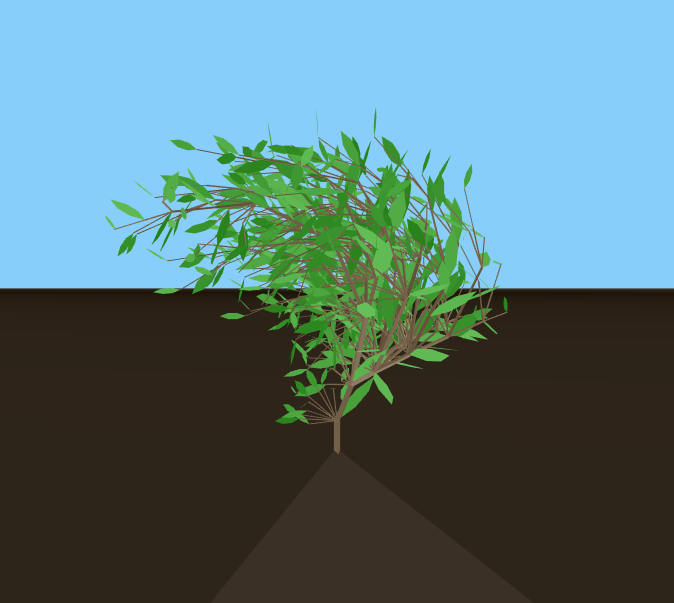
\includegraphics[width=\textwidth]{figures/plant-97}
        \caption{Survey plant 0.97}
    \end{subfigure}
    ~
    \begin{subfigure}{0.48\textwidth}
        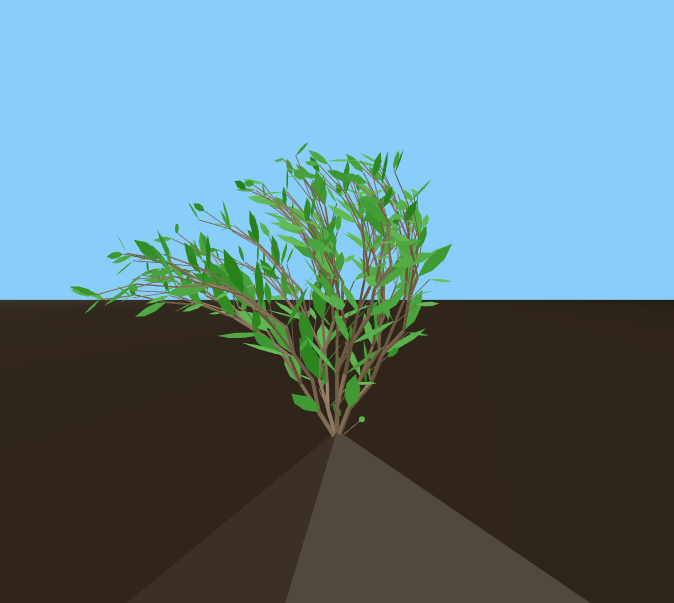
\includegraphics[width=\textwidth]{figures/plant-91}
        \caption{Survey plant 0.91}
    \end{subfigure}
    \\
    \begin{subfigure}{0.48\textwidth}
        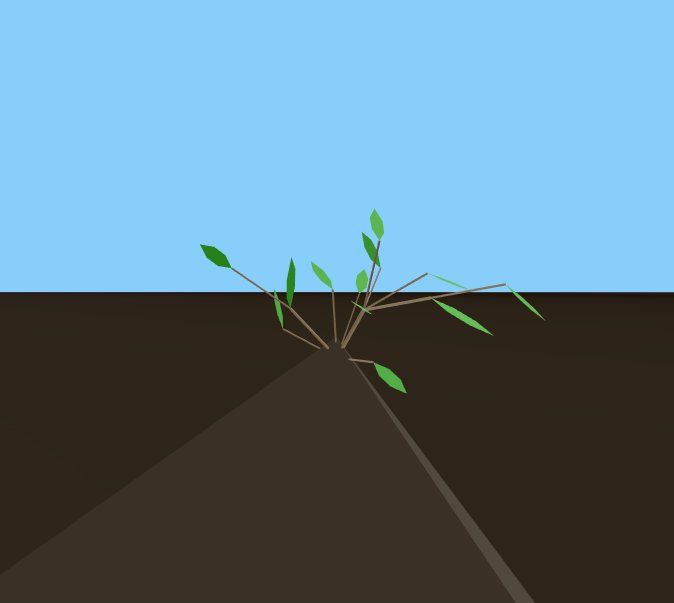
\includegraphics[width=\textwidth]{figures/plant-84}
        \caption{Survey plant 0.84}
    \end{subfigure}
    ~
    \begin{subfigure}{0.48\textwidth}
        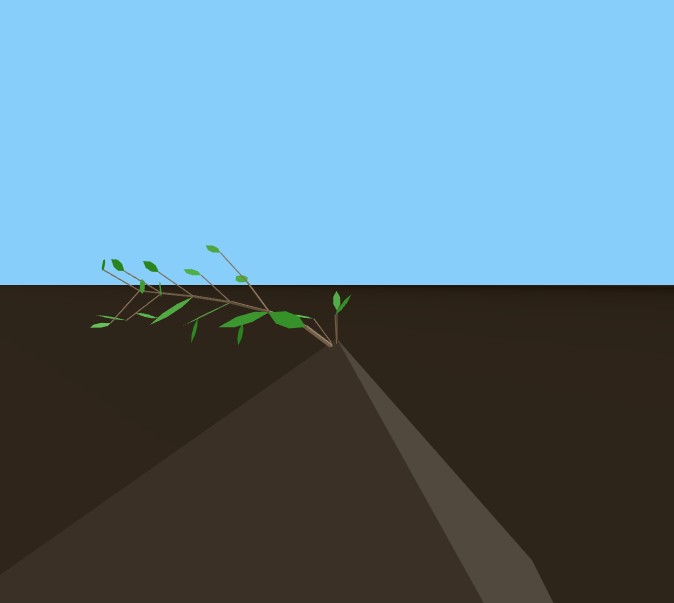
\includegraphics[width=\textwidth]{figures/plant-78}
        \caption{Survey plant 0.78}
    \end{subfigure}
    \\
    \begin{subfigure}{0.48\textwidth}
        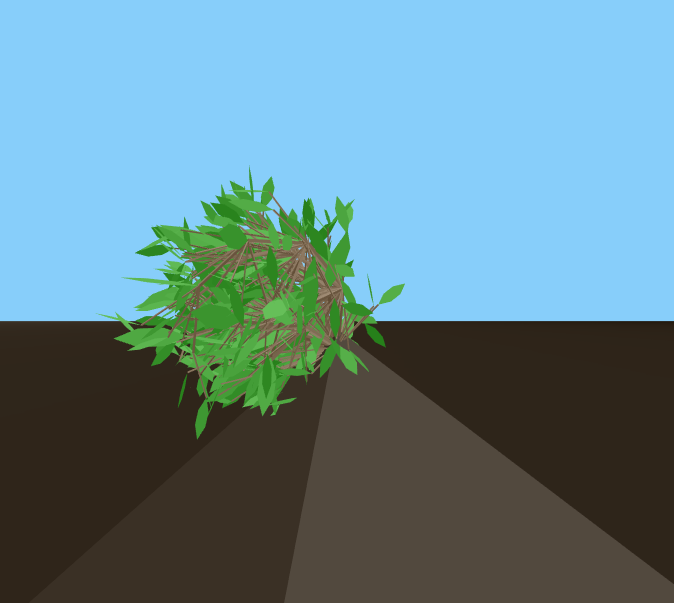
\includegraphics[width=\textwidth]{figures/plant-72}
        \caption{Survey plant 0.72}
    \end{subfigure}
    ~
    \begin{subfigure}{0.48\textwidth}
        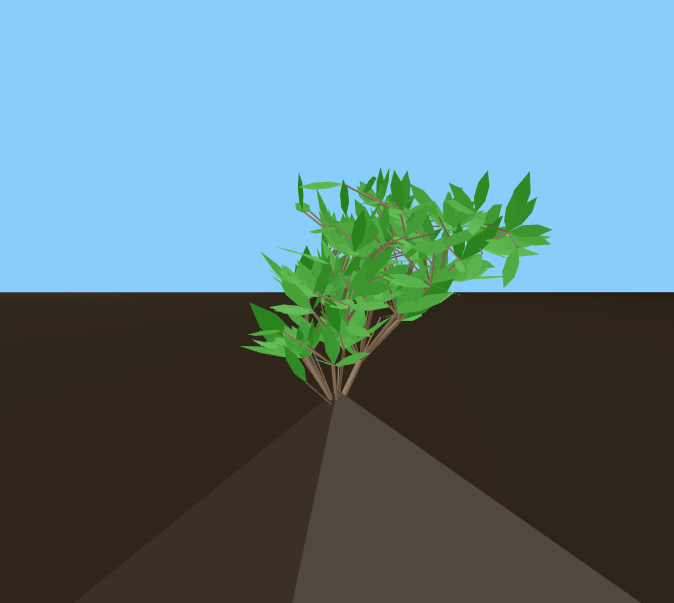
\includegraphics[width=\textwidth]{figures/plant-65}
        \caption{Survey plant 0.65}
    \end{subfigure}
\end{figure}
\begin{figure}
    \centering
    \begin{subfigure}{0.48\textwidth}
        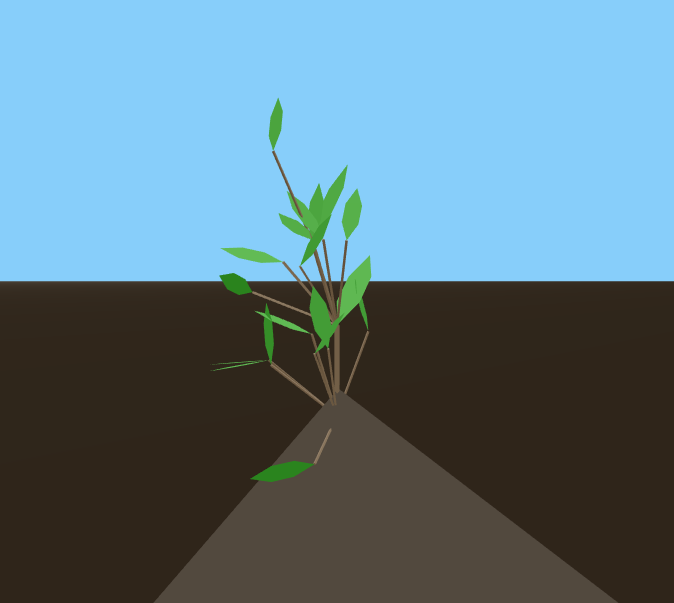
\includegraphics[width=\textwidth]{figures/plant-59}
        \caption{Survey plant 0.59}
    \end{subfigure}
    ~
    \begin{subfigure}{0.48\textwidth}
        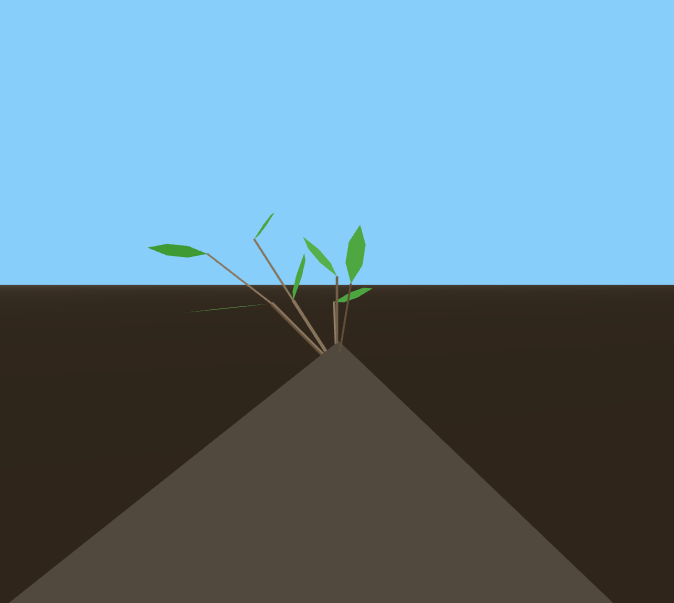
\includegraphics[width=\textwidth]{figures/plant-53}
        \caption{Survey plant 0.53}
    \end{subfigure}
    \\
    \begin{subfigure}{0.48\textwidth}
        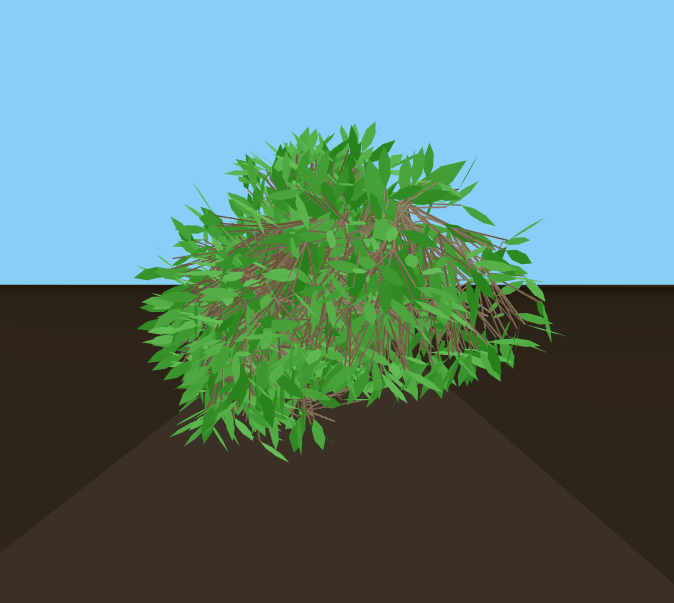
\includegraphics[width=\textwidth]{figures/plant-46}
        \caption{Survey plant 0.46}
    \end{subfigure}
    ~
    \begin{subfigure}{0.48\textwidth}
        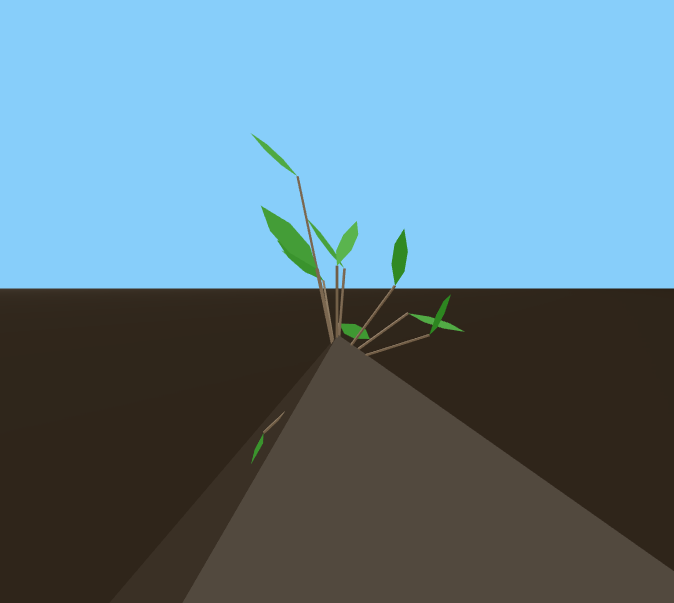
\includegraphics[width=\textwidth]{figures/plant-40}
        \caption{Survey plant 0.40}
    \end{subfigure}
    \\
    \begin{subfigure}{0.48\textwidth}
        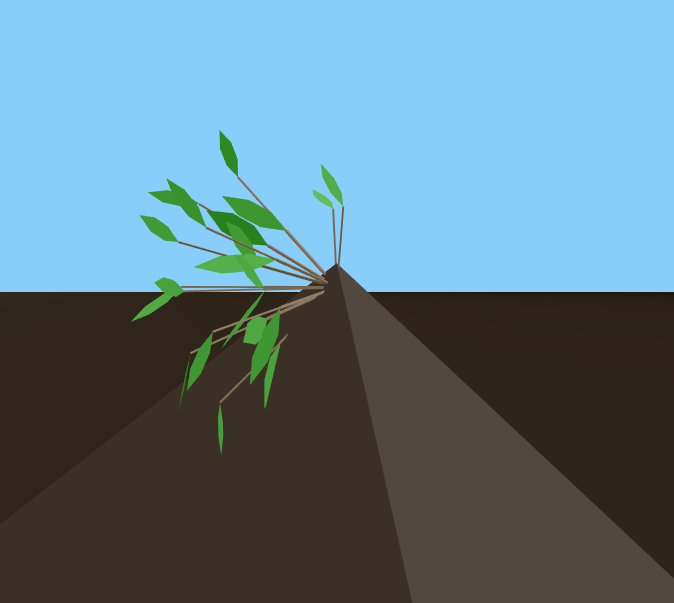
\includegraphics[width=\textwidth]{figures/plant-34}
        \caption{Survey plant 0.34}
    \end{subfigure}
    ~
    \begin{subfigure}{0.48\textwidth}
        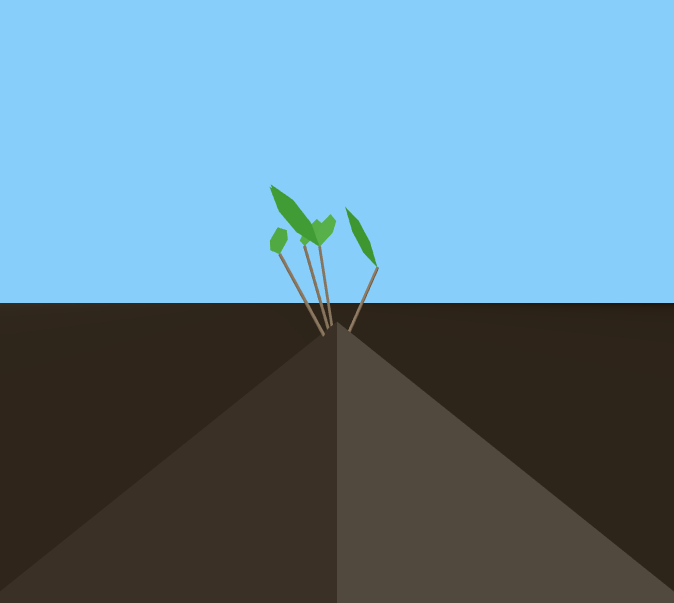
\includegraphics[width=\textwidth]{figures/plant-27}
        \caption{Survey plant 0.27}
    \end{subfigure}
    \ContinuedFloat
    \caption[All plants used in the survey]{All plants used in the survey, in descending rank order. Their name is equal to their fitness score.}
\end{figure}

% !TEX root = ../Masters.tex
\chapter{Various DGEL Generated Plants}
\label{app:plants}

The next page shows a collage of various hand-picked \gls{L-system} plants generated with \gls{DGEL}.

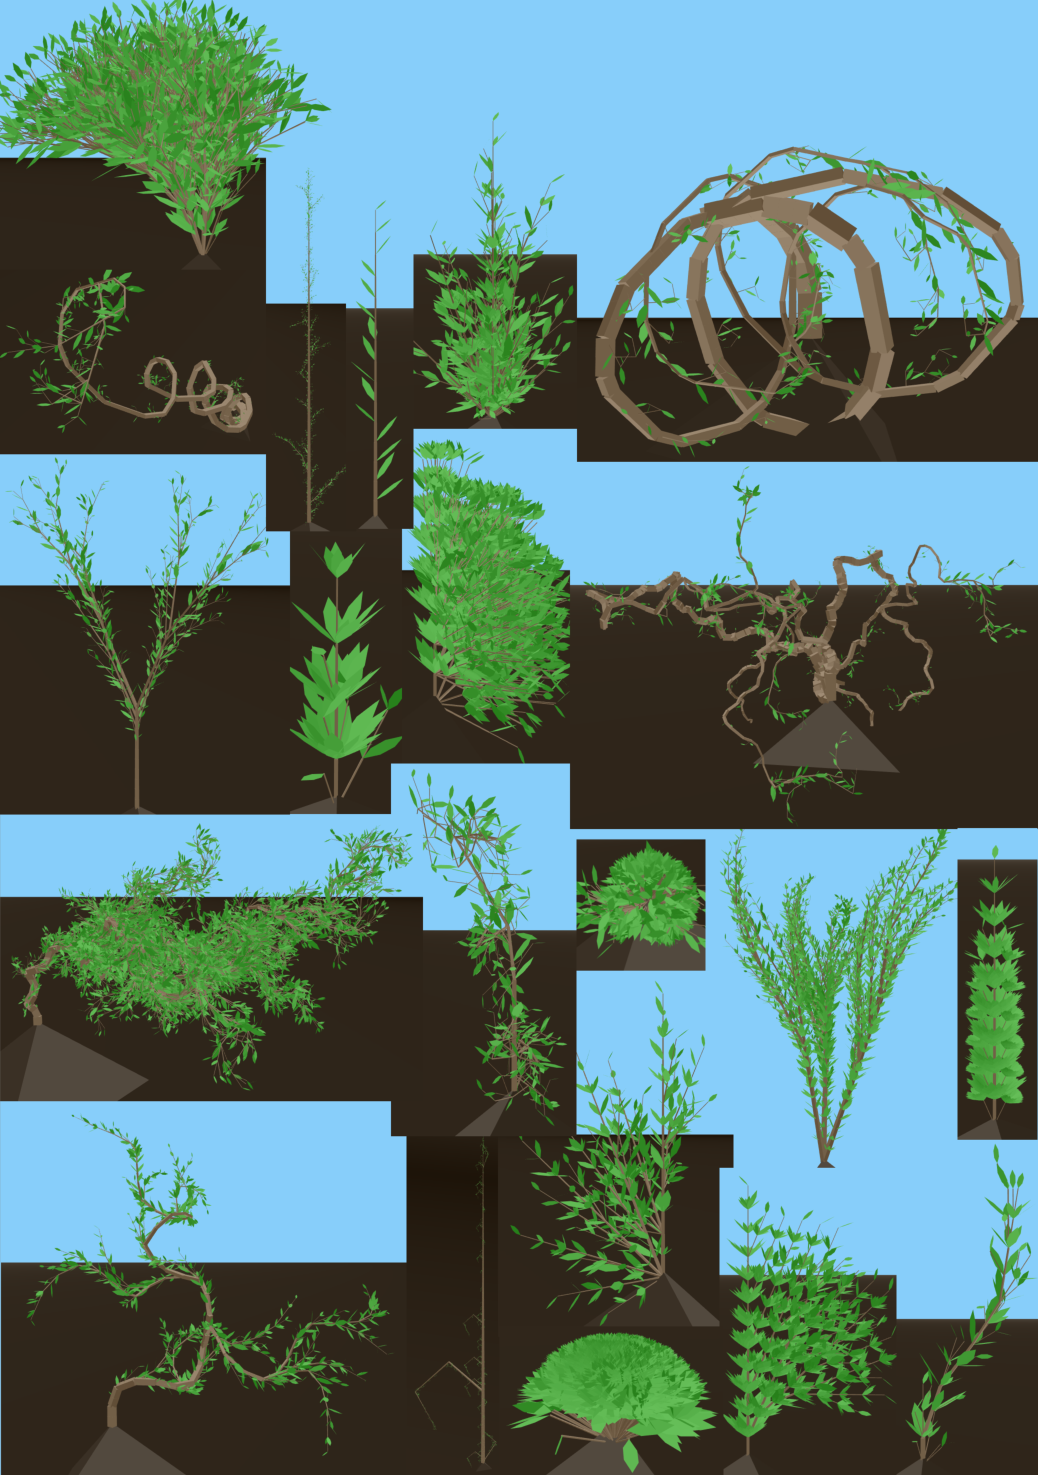
\includepdf{figures/plant_collage}


\end{document}
